\documentclass[11pt,]{article}
\usepackage[left=1in,top=1in,right=1in,bottom=1in]{geometry}
\newcommand*{\authorfont}{\fontfamily{phv}\selectfont}
\usepackage[]{mathpazo}
\usepackage{url}


  \usepackage[T1]{fontenc}
  \usepackage[utf8]{inputenc}



\usepackage{abstract}
\renewcommand{\abstractname}{}    % clear the title
\renewcommand{\absnamepos}{empty} % originally center

\renewenvironment{abstract}
 {{%
    \setlength{\leftmargin}{0mm}
    \setlength{\rightmargin}{\leftmargin}%
  }%
  \relax}
 {\endlist}

\makeatletter
\def\@maketitle{%
  \newpage
%  \null
%  \vskip 2em%
%  \begin{center}%
  \let \footnote \thanks
    {\fontsize{18}{20}\selectfont\raggedright  \setlength{\parindent}{0pt} \@title \par}%
}
%\fi
\makeatother




\setcounter{secnumdepth}{3}

\usepackage{color}
\usepackage{fancyvrb}
\newcommand{\VerbBar}{|}
\newcommand{\VERB}{\Verb[commandchars=\\\{\}]}
\DefineVerbatimEnvironment{Highlighting}{Verbatim}{commandchars=\\\{\}}
% Add ',fontsize=\small' for more characters per line
\usepackage{framed}
\definecolor{shadecolor}{RGB}{248,248,248}
\newenvironment{Shaded}{\begin{snugshade}}{\end{snugshade}}
\newcommand{\KeywordTok}[1]{\textcolor[rgb]{0.13,0.29,0.53}{\textbf{#1}}}
\newcommand{\DataTypeTok}[1]{\textcolor[rgb]{0.13,0.29,0.53}{#1}}
\newcommand{\DecValTok}[1]{\textcolor[rgb]{0.00,0.00,0.81}{#1}}
\newcommand{\BaseNTok}[1]{\textcolor[rgb]{0.00,0.00,0.81}{#1}}
\newcommand{\FloatTok}[1]{\textcolor[rgb]{0.00,0.00,0.81}{#1}}
\newcommand{\ConstantTok}[1]{\textcolor[rgb]{0.00,0.00,0.00}{#1}}
\newcommand{\CharTok}[1]{\textcolor[rgb]{0.31,0.60,0.02}{#1}}
\newcommand{\SpecialCharTok}[1]{\textcolor[rgb]{0.00,0.00,0.00}{#1}}
\newcommand{\StringTok}[1]{\textcolor[rgb]{0.31,0.60,0.02}{#1}}
\newcommand{\VerbatimStringTok}[1]{\textcolor[rgb]{0.31,0.60,0.02}{#1}}
\newcommand{\SpecialStringTok}[1]{\textcolor[rgb]{0.31,0.60,0.02}{#1}}
\newcommand{\ImportTok}[1]{#1}
\newcommand{\CommentTok}[1]{\textcolor[rgb]{0.56,0.35,0.01}{\textit{#1}}}
\newcommand{\DocumentationTok}[1]{\textcolor[rgb]{0.56,0.35,0.01}{\textbf{\textit{#1}}}}
\newcommand{\AnnotationTok}[1]{\textcolor[rgb]{0.56,0.35,0.01}{\textbf{\textit{#1}}}}
\newcommand{\CommentVarTok}[1]{\textcolor[rgb]{0.56,0.35,0.01}{\textbf{\textit{#1}}}}
\newcommand{\OtherTok}[1]{\textcolor[rgb]{0.56,0.35,0.01}{#1}}
\newcommand{\FunctionTok}[1]{\textcolor[rgb]{0.00,0.00,0.00}{#1}}
\newcommand{\VariableTok}[1]{\textcolor[rgb]{0.00,0.00,0.00}{#1}}
\newcommand{\ControlFlowTok}[1]{\textcolor[rgb]{0.13,0.29,0.53}{\textbf{#1}}}
\newcommand{\OperatorTok}[1]{\textcolor[rgb]{0.81,0.36,0.00}{\textbf{#1}}}
\newcommand{\BuiltInTok}[1]{#1}
\newcommand{\ExtensionTok}[1]{#1}
\newcommand{\PreprocessorTok}[1]{\textcolor[rgb]{0.56,0.35,0.01}{\textit{#1}}}
\newcommand{\AttributeTok}[1]{\textcolor[rgb]{0.77,0.63,0.00}{#1}}
\newcommand{\RegionMarkerTok}[1]{#1}
\newcommand{\InformationTok}[1]{\textcolor[rgb]{0.56,0.35,0.01}{\textbf{\textit{#1}}}}
\newcommand{\WarningTok}[1]{\textcolor[rgb]{0.56,0.35,0.01}{\textbf{\textit{#1}}}}
\newcommand{\AlertTok}[1]{\textcolor[rgb]{0.94,0.16,0.16}{#1}}
\newcommand{\ErrorTok}[1]{\textcolor[rgb]{0.64,0.00,0.00}{\textbf{#1}}}
\newcommand{\NormalTok}[1]{#1}
\usepackage{longtable,booktabs}

\usepackage{graphicx,grffile}
\makeatletter
\def\maxwidth{\ifdim\Gin@nat@width>\linewidth\linewidth\else\Gin@nat@width\fi}
\def\maxheight{\ifdim\Gin@nat@height>\textheight\textheight\else\Gin@nat@height\fi}
\makeatother
% Scale images if necessary, so that they will not overflow the page
% margins by default, and it is still possible to overwrite the defaults
% using explicit options in \includegraphics[width, height, ...]{}
\setkeys{Gin}{width=\maxwidth,height=\maxheight,keepaspectratio}

\title{Distribución espacial de los puntos de calor - Hot Spots para los
incendios forestales en la República Dominicana y predicción de las
zonas mas vulnerables usando el metodo de Kriging universal  }



\author{\Large Diego Cordero\vspace{0.05in} \newline\normalsize\emph{Estudiante de Maestría en Teledetección y Ciencias de la Información
Geográfica, Universidad Autónoma de Santo Domingo (UASD)}  }


\date{}

\usepackage{titlesec}

\titleformat*{\section}{\normalsize\bfseries}
\titleformat*{\subsection}{\normalsize\itshape}
\titleformat*{\subsubsection}{\normalsize\itshape}
\titleformat*{\paragraph}{\normalsize\itshape}
\titleformat*{\subparagraph}{\normalsize\itshape}

\titlespacing{\section}
{0pt}{36pt}{0pt}
\titlespacing{\subsection}
{0pt}{36pt}{0pt}
\titlespacing{\subsubsection}
{0pt}{36pt}{0pt}





\newtheorem{hypothesis}{Hypothesis}
\usepackage{setspace}

\makeatletter
\@ifpackageloaded{hyperref}{}{%
\ifxetex
  \PassOptionsToPackage{hyphens}{url}\usepackage[setpagesize=false, % page size defined by xetex
              unicode=false, % unicode breaks when used with xetex
              xetex]{hyperref}
\else
  \PassOptionsToPackage{hyphens}{url}\usepackage[unicode=true]{hyperref}
\fi
}

\@ifpackageloaded{color}{
    \PassOptionsToPackage{usenames,dvipsnames}{color}
}{%
    \usepackage[usenames,dvipsnames]{color}
}
\makeatother
\hypersetup{breaklinks=true,
            bookmarks=true,
            pdfauthor={Diego Cordero (Estudiante de Maestría en Teledetección y Ciencias de la Información
Geográfica, Universidad Autónoma de Santo Domingo (UASD))},
             pdfkeywords = {r, rstudio, fire forest, incendio forestal, kriging, LISA cluster},  
            pdftitle={Distribución espacial de los puntos de calor - Hot Spots para los
incendios forestales en la República Dominicana y predicción de las
zonas mas vulnerables usando el metodo de Kriging universal},
            colorlinks=true,
            citecolor=blue,
            urlcolor=blue,
            linkcolor=magenta,
            pdfborder={0 0 0}}
\urlstyle{same}  % don't use monospace font for urls

% set default figure placement to htbp
\makeatletter
\def\fps@figure{htbp}
\makeatother

\usepackage{pdflscape} \newcommand{\blandscape}{\begin{landscape}}
\newcommand{\elandscape}{\end{landscape}}


% add tightlist ----------
\providecommand{\tightlist}{%
\setlength{\itemsep}{0pt}\setlength{\parskip}{0pt}}

\begin{document}
	
% \pagenumbering{arabic}% resets `page` counter to 1 
%
% \maketitle

{% \usefont{T1}{pnc}{m}{n}
\setlength{\parindent}{0pt}
\thispagestyle{plain}
{\fontsize{18}{20}\selectfont\raggedright 
\maketitle  % title \par  

}

{
   \vskip 13.5pt\relax \normalsize\fontsize{11}{12} 
\textbf{\authorfont Diego Cordero} \hskip 15pt \emph{\small Estudiante de Maestría en Teledetección y Ciencias de la Información
Geográfica, Universidad Autónoma de Santo Domingo (UASD)}   

}

}








\begin{abstract}

    \hbox{\vrule height .2pt width 39.14pc}

    \vskip 8.5pt % \small 

\noindent Esta investigación se basa en información geográfica de libre acceso
encontrada en la web y pretende realizar un análisis geoespacial que
permita conocer cuál es la distribución espacial de los puntos de calor
- Hot Spots para los incendios forestales en la República Dominicana.
Para lo cual se descargó la información correspondiente para el periodo
2009-2019 de la pagina de NASA-FIRMS (2020). El resultado final esperado
que se busca mediante el desarrollo de un script bajo el software R y la
herramienta RStudio es un Cluster LISA que indique la relación espacial
de los municipios con los incendios y una predicción de las zonas mas
vulnerables usando el metodo de Kriging universal teniendo como base la
elevación de un modelo digital de elevación (DEM).


\vskip 8.5pt \noindent \emph{Keywords}: r, rstudio, fire forest, incendio forestal, kriging, LISA cluster \par

    \hbox{\vrule height .2pt width 39.14pc}



\end{abstract}


\vskip 6.5pt


\noindent  \section{Introducción}\label{introducciuxf3n}

Los incendios forestales son un problema mundial, por lo que mediante
este estudio se espera realizar un acercamiento para dar conocer a
mediante el uso de análisis geoestadisticos las posibles causas de
variables naturales que pueden influir en la propagación de los mismos.
Mediante herramientas y data de libre acceso se pretende realizar un
acercamiento que permita establecer la relación directa o indirecta
sobre la problemática principal que se ha intesificado durante el 2019
según Diario Libre (2019) siendo Los parques nacionales los más
quemados, el mismo establece que para los primeros meses de 2019 tuvo un
incremento en los incendios Vs 2018. El gobierno dominicano entre las
medidas preventivas previstas en cabeza del Ministerio de Medio Ambiente
y Recursos Naturales, en coordinación con ministerio de Obras Publicas y
el ministerio de Defensa, activó un Plan Preventivo de Emergencia (PPE)
en la que se sobrevolará en helicópteros y drones las zonas vulnerables
donde se producen conatos de incendio por conuquismo, con el propósito
de detectar los daños en los bosques, atrapar a los culpables y actuar
contra los responsables asegura EFE (2019).

\section{Metodología}\label{metodologuxeda}

\subsection{Librerias Necesarias y adición de
data}\label{librerias-necesarias-y-adiciuxf3n-de-data}

Inicialmente se usarán las siguientes librerías y el archivo para el
desarrollo de los LISA cluster realizado por Martínez Batlle (2019c)
para el desarrollo del script para la investigación

\begin{Shaded}
\begin{Highlighting}[]
\KeywordTok{library}\NormalTok{(sf)}
\KeywordTok{library}\NormalTok{(sp)}
\KeywordTok{library}\NormalTok{(raster)}
\KeywordTok{library}\NormalTok{(tidyverse)}
\KeywordTok{library}\NormalTok{(tmap)}
\KeywordTok{library}\NormalTok{(RColorBrewer)}
\KeywordTok{library}\NormalTok{(lmtest)}
\KeywordTok{library}\NormalTok{(spdep)}
\KeywordTok{library}\NormalTok{(parallel)}
\KeywordTok{library}\NormalTok{(ggplot2)}
\KeywordTok{library}\NormalTok{(gstat)}
\KeywordTok{library}\NormalTok{(stars)}
\KeywordTok{source}\NormalTok{(}\StringTok{'lisaclusters.R'}\NormalTok{)}
\end{Highlighting}
\end{Shaded}

Teniendo en cuenta la información disponible se realizó la carga de la
data de \textbf{incendios, municipios, y uso de suelo}, la primera de
las capas fue trabajada inicialmente en QGis realizando un join de la
data de VIIRS y MODIS, sin embargo se percibieron dos problemas. La
cantidad de zonas de alta densidad de incendios que correspondían a
canteras y zonas industriales a lo largo del país como se presenta en
las Figuras 1 y en segunda instancia la notoriedad que no todos los
incendios correspondian a incendios forestales.

\begin{figure}
\centering
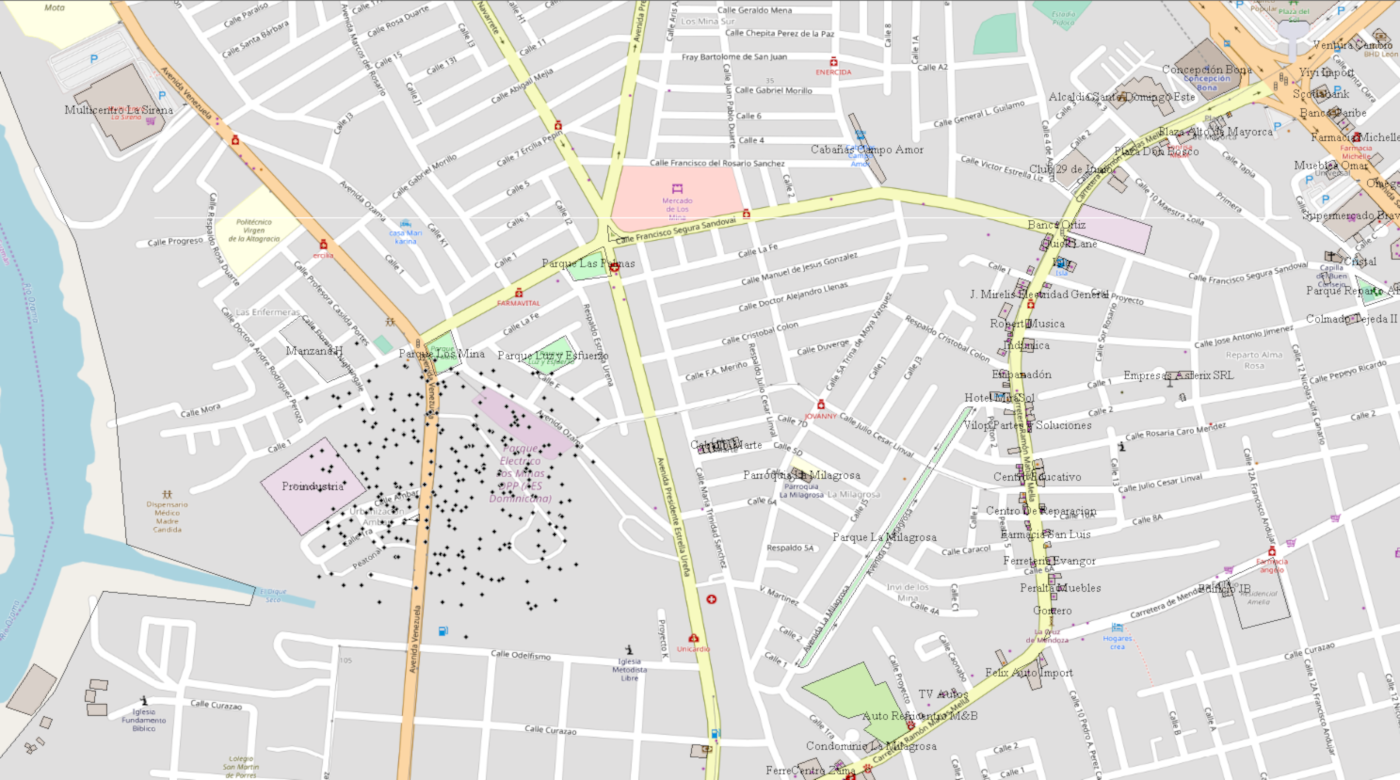
\includegraphics{proyecto_files/Imagenes/BuildingPoints.png}
\caption{Densidad de Incendios en zonas Industriales}
\end{figure}

Para el primer problema y haciendo uso de la data de la OpenStreetMaps
(2020), se realizo un buffer de los centroides de los poligonos de
canteras y edificios de un radio de 1.11 km o 0.01 grados teniendo en
cuenta que la data se encuentra en la referencia espacial WGS84:4326
usando el archivo \texttt{gis\_osm\_landuse\_a\_free\_1} eliminando
todos los datos que se encontrarán dentro del mismo como se muestra en
la Figura 2.

\begin{figure}
\centering
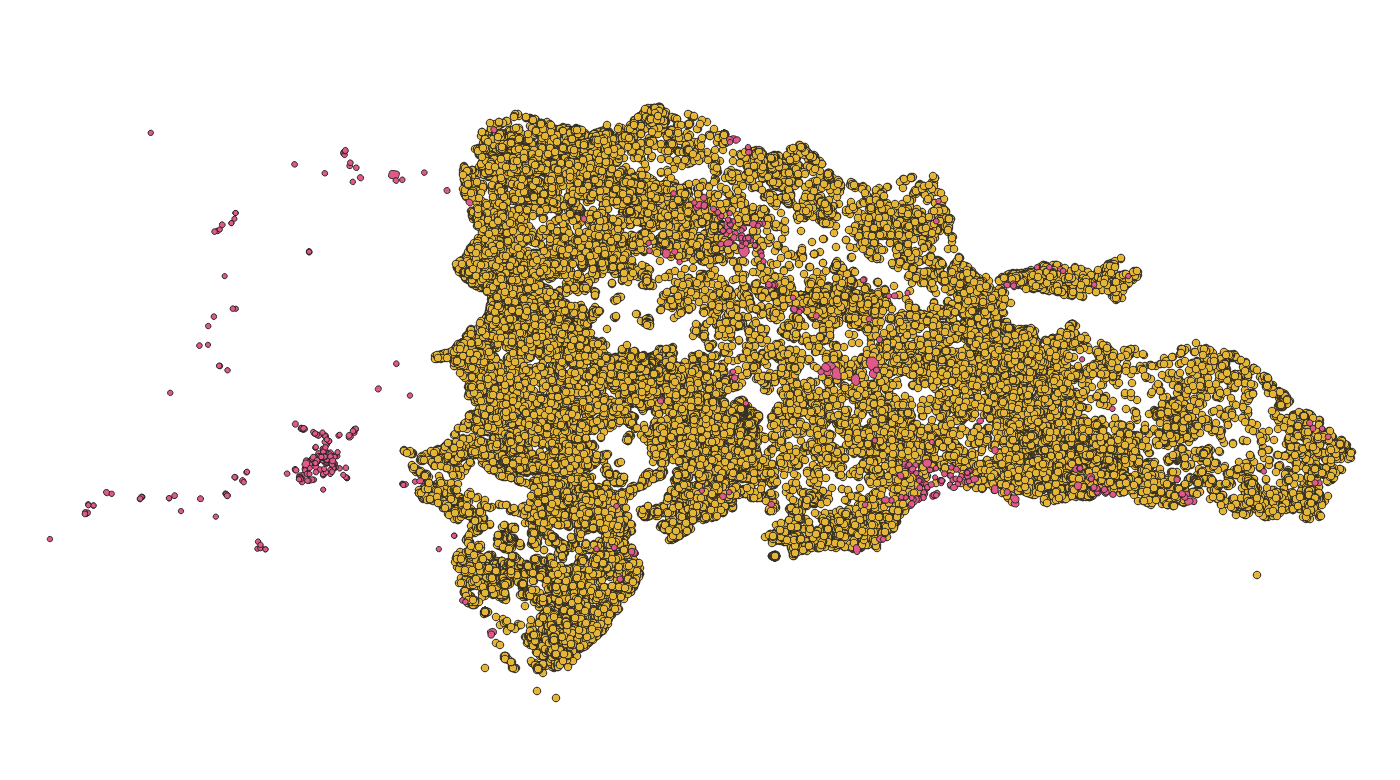
\includegraphics{proyecto_files/Imagenes/Buffer.png}
\caption{Resultado Buffer}
\end{figure}

Para el segundo problema y haciendo uso de la data de GlobCover (2005)
se realizó un subset de los usos de suelo contemplando los valores entre
30 y 120 de la siguiente tabla tomada de la data descargada de
GlobCover.

\begin{longtable}[]{@{}ll@{}}
\toprule
\begin{minipage}[b]{0.08\columnwidth}\raggedright\strut
Value\strut
\end{minipage} & \begin{minipage}[b]{0.86\columnwidth}\raggedright\strut
Label\strut
\end{minipage}\tabularnewline
\midrule
\endhead
\begin{minipage}[t]{0.08\columnwidth}\raggedright\strut
11\strut
\end{minipage} & \begin{minipage}[t]{0.86\columnwidth}\raggedright\strut
Post-flooding or irrigated croplands (or aquatic)\strut
\end{minipage}\tabularnewline
\begin{minipage}[t]{0.08\columnwidth}\raggedright\strut
14\strut
\end{minipage} & \begin{minipage}[t]{0.86\columnwidth}\raggedright\strut
Rainfed croplands\strut
\end{minipage}\tabularnewline
\begin{minipage}[t]{0.08\columnwidth}\raggedright\strut
20\strut
\end{minipage} & \begin{minipage}[t]{0.86\columnwidth}\raggedright\strut
Mosaic cropland (50-70\%) / vegetation (grassland/shrubland/forest)
(20-50\%)\strut
\end{minipage}\tabularnewline
\begin{minipage}[t]{0.08\columnwidth}\raggedright\strut
30\strut
\end{minipage} & \begin{minipage}[t]{0.86\columnwidth}\raggedright\strut
Mosaic vegetation (grassland/shrubland/forest) (50-70\%) / cropland
(20-50\%)\strut
\end{minipage}\tabularnewline
\begin{minipage}[t]{0.08\columnwidth}\raggedright\strut
40\strut
\end{minipage} & \begin{minipage}[t]{0.86\columnwidth}\raggedright\strut
Closed to open (\textgreater{}15\%) broadleaved evergreen or
semi-deciduous forest (\textgreater{}5m)\strut
\end{minipage}\tabularnewline
\begin{minipage}[t]{0.08\columnwidth}\raggedright\strut
50\strut
\end{minipage} & \begin{minipage}[t]{0.86\columnwidth}\raggedright\strut
Closed (\textgreater{}40\%) broadleaved deciduous forest
(\textgreater{}5m)\strut
\end{minipage}\tabularnewline
\begin{minipage}[t]{0.08\columnwidth}\raggedright\strut
60\strut
\end{minipage} & \begin{minipage}[t]{0.86\columnwidth}\raggedright\strut
Open (15-40\%) broadleaved deciduous forest/woodland
(\textgreater{}5m)\strut
\end{minipage}\tabularnewline
\begin{minipage}[t]{0.08\columnwidth}\raggedright\strut
70\strut
\end{minipage} & \begin{minipage}[t]{0.86\columnwidth}\raggedright\strut
Closed (\textgreater{}40\%) needleleaved evergreen forest
(\textgreater{}5m)\strut
\end{minipage}\tabularnewline
\begin{minipage}[t]{0.08\columnwidth}\raggedright\strut
90\strut
\end{minipage} & \begin{minipage}[t]{0.86\columnwidth}\raggedright\strut
Open (15-40\%) needleleaved deciduous or evergreen forest
(\textgreater{}5m)\strut
\end{minipage}\tabularnewline
\begin{minipage}[t]{0.08\columnwidth}\raggedright\strut
100\strut
\end{minipage} & \begin{minipage}[t]{0.86\columnwidth}\raggedright\strut
Closed to open (\textgreater{}15\%) mixed broadleaved and needleleaved
forest (\textgreater{}5m)\strut
\end{minipage}\tabularnewline
\begin{minipage}[t]{0.08\columnwidth}\raggedright\strut
110\strut
\end{minipage} & \begin{minipage}[t]{0.86\columnwidth}\raggedright\strut
Mosaic forest or shrubland (50-70\%) / grassland (20-50\%)\strut
\end{minipage}\tabularnewline
\begin{minipage}[t]{0.08\columnwidth}\raggedright\strut
120\strut
\end{minipage} & \begin{minipage}[t]{0.86\columnwidth}\raggedright\strut
Mosaic grassland (50-70\%) / forest or shrubland (20-50\%)\strut
\end{minipage}\tabularnewline
\begin{minipage}[t]{0.08\columnwidth}\raggedright\strut
130\strut
\end{minipage} & \begin{minipage}[t]{0.86\columnwidth}\raggedright\strut
Closed to open (\textgreater{}15\%) (broadleaved or needleleaved,
evergreen or deciduous) shrubland (\textless{}5m)\strut
\end{minipage}\tabularnewline
\begin{minipage}[t]{0.08\columnwidth}\raggedright\strut
140\strut
\end{minipage} & \begin{minipage}[t]{0.86\columnwidth}\raggedright\strut
Closed to open (\textgreater{}15\%) herbaceous vegetation (grassland,
savannas or lichens/mosses)\strut
\end{minipage}\tabularnewline
\begin{minipage}[t]{0.08\columnwidth}\raggedright\strut
150\strut
\end{minipage} & \begin{minipage}[t]{0.86\columnwidth}\raggedright\strut
Sparse (\textless{}15\%) vegetation\strut
\end{minipage}\tabularnewline
\begin{minipage}[t]{0.08\columnwidth}\raggedright\strut
160\strut
\end{minipage} & \begin{minipage}[t]{0.86\columnwidth}\raggedright\strut
Closed to open (\textgreater{}15\%) broadleaved forest regularly flooded
(semi-permanently or temporarily) - Fresh or brackish water\strut
\end{minipage}\tabularnewline
\begin{minipage}[t]{0.08\columnwidth}\raggedright\strut
170\strut
\end{minipage} & \begin{minipage}[t]{0.86\columnwidth}\raggedright\strut
Closed (\textgreater{}40\%) broadleaved forest or shrubland permanently
flooded - Saline or brackish water\strut
\end{minipage}\tabularnewline
\begin{minipage}[t]{0.08\columnwidth}\raggedright\strut
180\strut
\end{minipage} & \begin{minipage}[t]{0.86\columnwidth}\raggedright\strut
Closed to open (\textgreater{}15\%) grassland or woody vegetation on
regularly flooded or waterlogged soil - Fresh, brackish or saline
water\strut
\end{minipage}\tabularnewline
\begin{minipage}[t]{0.08\columnwidth}\raggedright\strut
190\strut
\end{minipage} & \begin{minipage}[t]{0.86\columnwidth}\raggedright\strut
Artificial surfaces and associated areas (Urban areas
\textgreater{}50\%)\strut
\end{minipage}\tabularnewline
\begin{minipage}[t]{0.08\columnwidth}\raggedright\strut
200\strut
\end{minipage} & \begin{minipage}[t]{0.86\columnwidth}\raggedright\strut
Bare areas\strut
\end{minipage}\tabularnewline
\begin{minipage}[t]{0.08\columnwidth}\raggedright\strut
210\strut
\end{minipage} & \begin{minipage}[t]{0.86\columnwidth}\raggedright\strut
Water bodies\strut
\end{minipage}\tabularnewline
\begin{minipage}[t]{0.08\columnwidth}\raggedright\strut
220\strut
\end{minipage} & \begin{minipage}[t]{0.86\columnwidth}\raggedright\strut
Permanent snow and ice\strut
\end{minipage}\tabularnewline
\begin{minipage}[t]{0.08\columnwidth}\raggedright\strut
230\strut
\end{minipage} & \begin{minipage}[t]{0.86\columnwidth}\raggedright\strut
No data (burnt areas, clouds,\ldots{})\strut
\end{minipage}\tabularnewline
\bottomrule
\end{longtable}

Se realizó una comprobación para conocer si los valores correspondían a
los usados para la obtención de los datos forestales y se realizo una
intersección entre la capa de incendios y la de municipios asignandole a
cada dato el valor ENLACE.

\begin{verbatim}
##    Min. 1st Qu.  Median    Mean 3rd Qu.    Max. 
##   30.00   30.00   30.00   37.91   40.00  120.00
\end{verbatim}

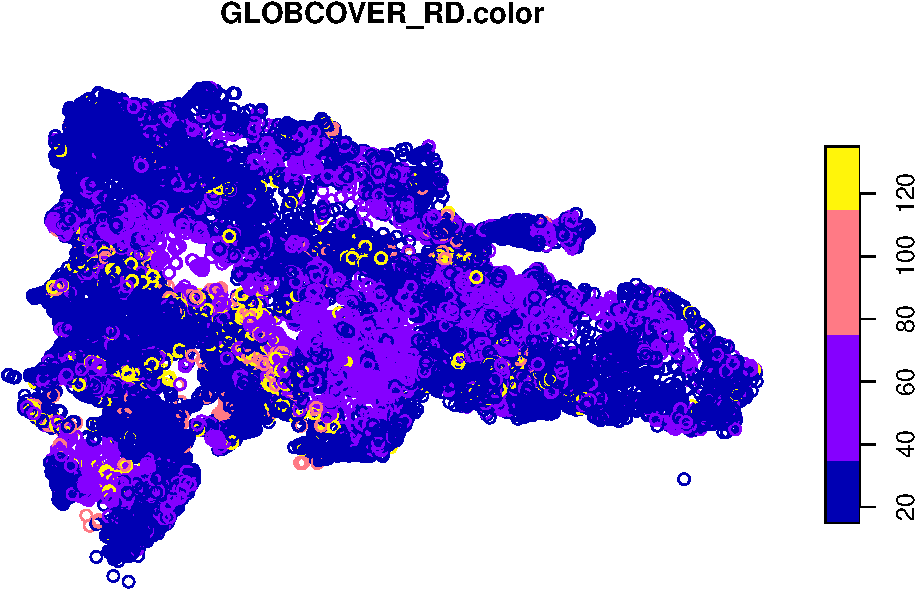
\includegraphics{proyecto_files/figure-latex/unnamed-chunk-6-1.pdf}

Con la información resulante para cada dato, se realizó un arrange entre
el numero de datos con el mismo ENLACE y se concatenó con la data de
municipios permitiendo así mostrar un mapa con la cantidad de incendios
por municipio.

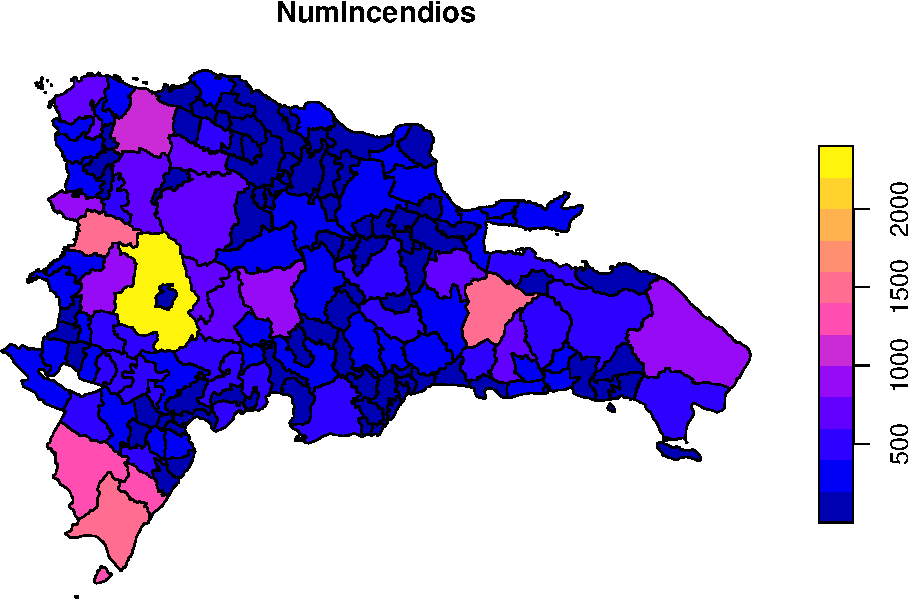
\includegraphics{proyecto_files/figure-latex/unnamed-chunk-8-1.pdf}

\subsection{Vecindad}\label{vecindad}

Para hallar los vecinos, se debe convertir la capa de Incedios por
Municipio a \texttt{SpatialPolygonsDataFrame}, y basado en el anterior
se crea un objeto de vecindad por contigüidad usando el criterio
\texttt{queen}, dandonos como resultado el mapa de vinculos de vecindad
de cada municipio,

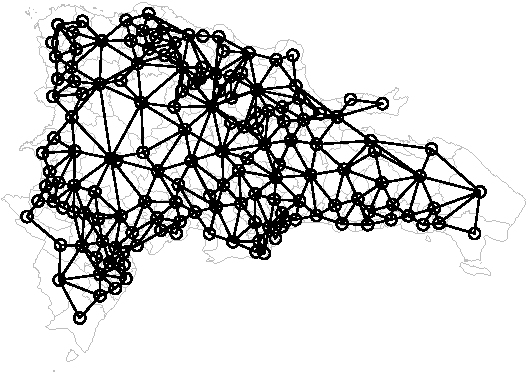
\includegraphics{proyecto_files/figure-latex/unnamed-chunk-10-1.pdf}

Sin embargo se debe hallar los vinculos de vecindad entre los municipios
para lo que se usa su vecino mas proximo

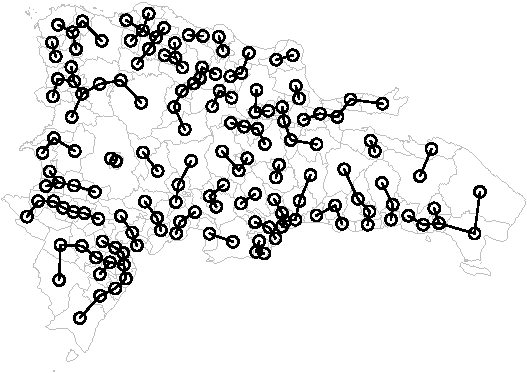
\includegraphics{proyecto_files/figure-latex/unnamed-chunk-12-1.pdf}

Basandose en el mapa resultante se visualizan los datos estadísticos
descriptivos sobre las distancias entre los municipios permitiendo
determinar los valores extremos (mínimo y máximo) de distancias a
vecinos más próximos.

\begin{Shaded}
\begin{Highlighting}[]
\KeywordTok{summary}\NormalTok{(dist)}
\end{Highlighting}
\end{Shaded}

\begin{verbatim}
##    Min. 1st Qu.  Median    Mean 3rd Qu.    Max. 
## 0.04036 0.08754 0.10140 0.11396 0.12765 0.28058
\end{verbatim}

\begin{Shaded}
\begin{Highlighting}[]
\KeywordTok{hist}\NormalTok{(dist)}
\end{Highlighting}
\end{Shaded}

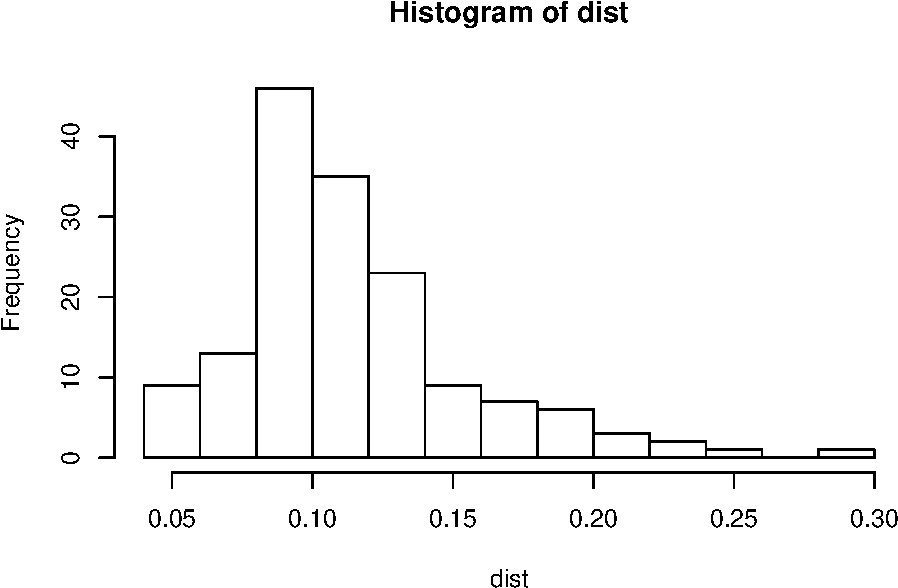
\includegraphics{proyecto_files/figure-latex/unnamed-chunk-14-1.pdf}

\begin{Shaded}
\begin{Highlighting}[]
\KeywordTok{boxplot}\NormalTok{(dist)}
\end{Highlighting}
\end{Shaded}

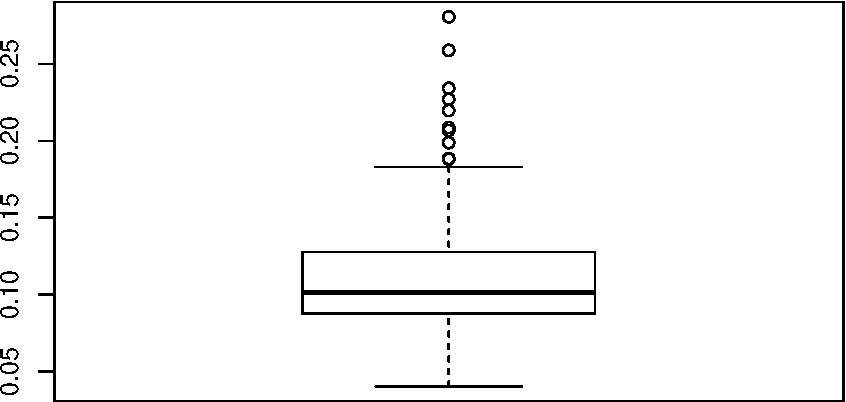
\includegraphics{proyecto_files/figure-latex/unnamed-chunk-14-2.pdf}

A continuación deben asignarse los pesos espaciales utilizando el estilo
\emph{weighted} o ``W'', donde los pesos de las observaciones vecinas a
una observación dada, suman 1, asignando pesos homogéneos a cada vecino,
sin embargo se realizará tambien al estilo binario. (Bivand, Pebesma, \&
Gomez-Rubio, 2008), bajo el cual el objeto \emph{j} recibe un peso de
\emph{1} ante el objeto \emph{i}, siempre que el primero sea vecino del
primero; por el contrario, si \emph{k} no es vecino de \emph{i} recibe
un peso de 0 por ante \emph{i}. Los pesos son indicativos de la
fortaleza de la relación entre dos o más observaciones.

\begin{Shaded}
\begin{Highlighting}[]
\NormalTok{munInc.w.W }
\end{Highlighting}
\end{Shaded}

\begin{verbatim}
## Characteristics of weights list object:
## Neighbour list object:
## Number of regions: 155 
## Number of nonzero links: 804 
## Percentage nonzero weights: 3.346514 
## Average number of links: 5.187097 
## 
## Weights style: W 
## Weights constants summary:
##     n    nn  S0       S1       S2
## W 155 24025 155 65.94606 650.7687
\end{verbatim}

\begin{Shaded}
\begin{Highlighting}[]
\NormalTok{munInc.w.B}
\end{Highlighting}
\end{Shaded}

\begin{verbatim}
## Characteristics of weights list object:
## Neighbour list object:
## Number of regions: 155 
## Number of nonzero links: 804 
## Percentage nonzero weights: 3.346514 
## Average number of links: 5.187097 
## 
## Weights style: B 
## Weights constants summary:
##     n    nn  S0   S1    S2
## B 155 24025 804 1608 19520
\end{verbatim}

\subsection{Autocorrelación espacial}\label{autocorrelaciuxf3n-espacial}

Para trabajar en la autocorrelación espacial se decide generar varias
columnas entre las que se encuentran \emph{porcentaje de incendios} y
\emph{porcentaje por km2} a su vez y puesto que existen municipios mas
grandes que otros y esto puede generar valores erroneos para el estudio
se generan una columna de \emph{incendios por area}, sin embargo para
efectos de estudio se genera una columna usando el \emph{logaritmo},
\emph{Ladder of Powers (escalera de potencias de Tukey)} y
\emph{tukey\_lamda}

\begin{verbatim}
## 
##     lambda      W Shapiro.p.value
## 409    0.2 0.9944          0.8194
## 
## if (lambda >  0){TRANS = x ^ lambda} 
## if (lambda == 0){TRANS = log(x)} 
## if (lambda <  0){TRANS = -1 * x ^ lambda}
\end{verbatim}

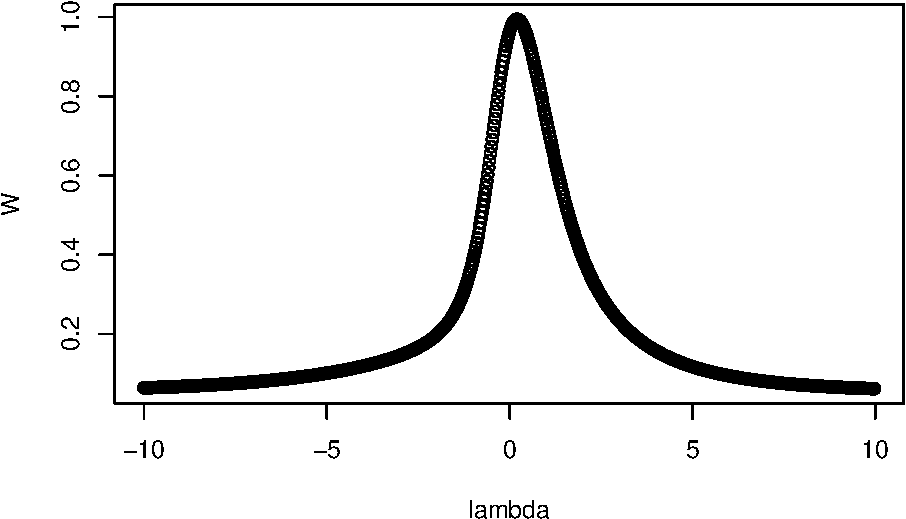
\includegraphics{proyecto_files/figure-latex/unnamed-chunk-18-1.pdf}

\begin{verbatim}
## 
##     lambda      W Shapiro.p.value
## 409    0.2 0.9944          0.8194
## 
## if (lambda >  0){TRANS = x ^ lambda} 
## if (lambda == 0){TRANS = log(x)} 
## if (lambda <  0){TRANS = -1 * x ^ lambda}
\end{verbatim}

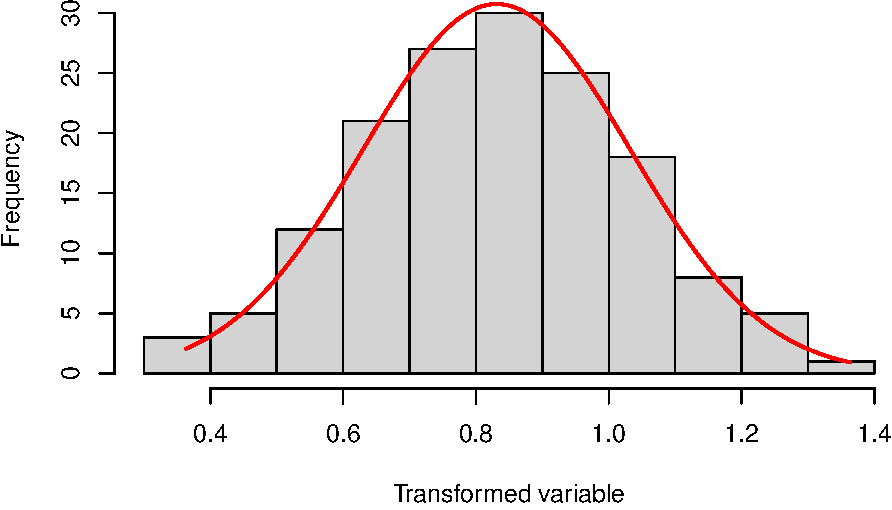
\includegraphics{proyecto_files/figure-latex/unnamed-chunk-18-2.pdf}
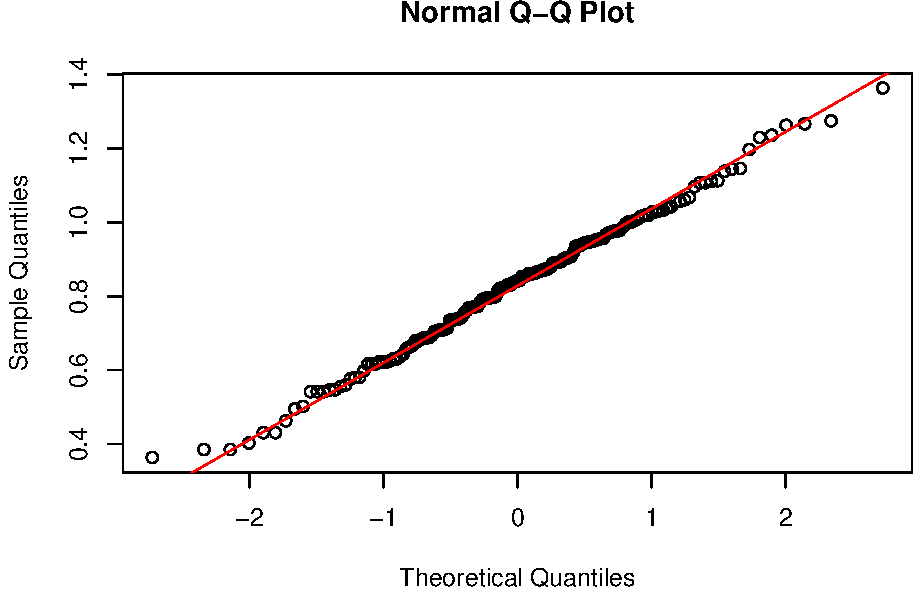
\includegraphics{proyecto_files/figure-latex/unnamed-chunk-18-3.pdf}

\begin{verbatim}
## 
##     lambda      W Shapiro.p.value
## 413    0.3 0.9956          0.9253
## 
## if (lambda >  0){TRANS = x ^ lambda} 
## if (lambda == 0){TRANS = log(x)} 
## if (lambda <  0){TRANS = -1 * x ^ lambda}
\end{verbatim}

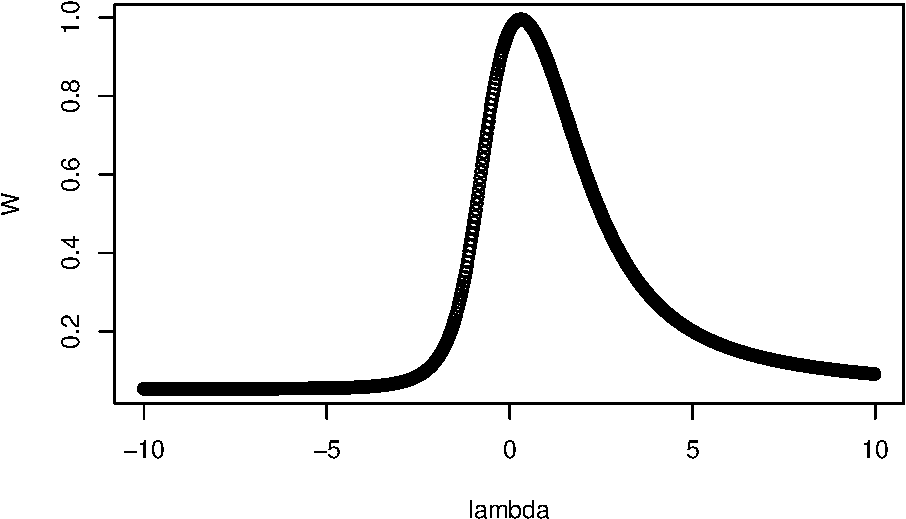
\includegraphics{proyecto_files/figure-latex/unnamed-chunk-18-4.pdf}

\begin{verbatim}
## 
##     lambda      W Shapiro.p.value
## 413    0.3 0.9956          0.9253
## 
## if (lambda >  0){TRANS = x ^ lambda} 
## if (lambda == 0){TRANS = log(x)} 
## if (lambda <  0){TRANS = -1 * x ^ lambda}
\end{verbatim}

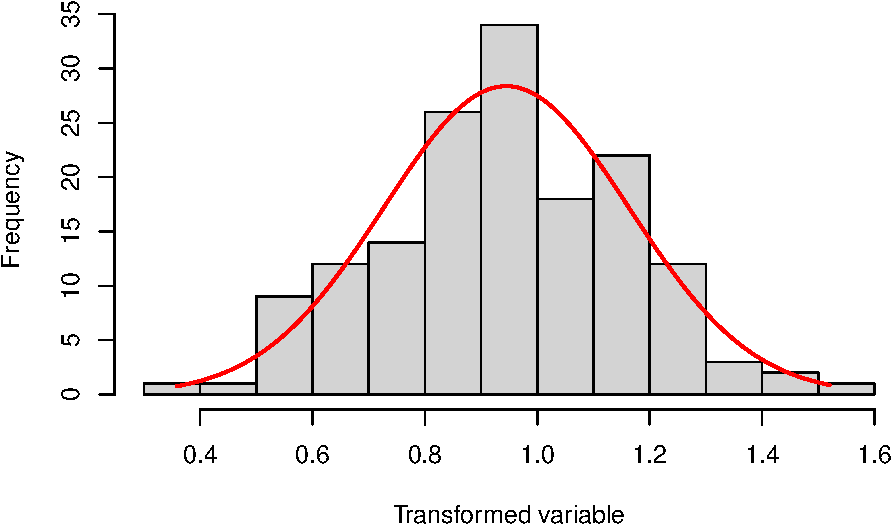
\includegraphics{proyecto_files/figure-latex/unnamed-chunk-18-5.pdf}
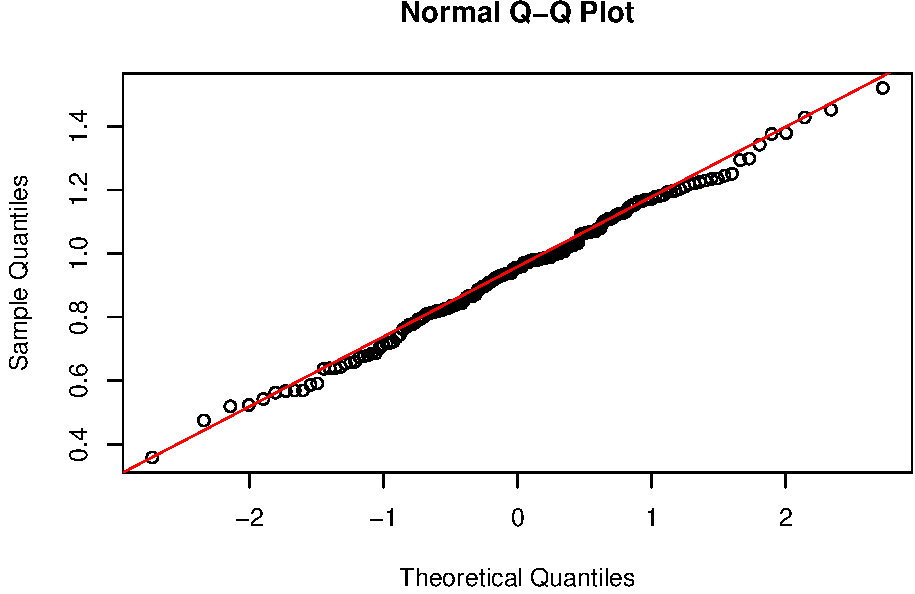
\includegraphics{proyecto_files/figure-latex/unnamed-chunk-18-6.pdf}

Teniendo en cuenta los resultados se genera el poligono realizando una
union entre Incendios por Municipio y la tabla resultante anterior.

Basandose en la capa resultante se realizan dos mapas que representan
los porcentajes de incendios por cada municipio sin importar el área
mostrando a los municipios del sur oeste y San Juan como los de mayor
tasa de incendios.

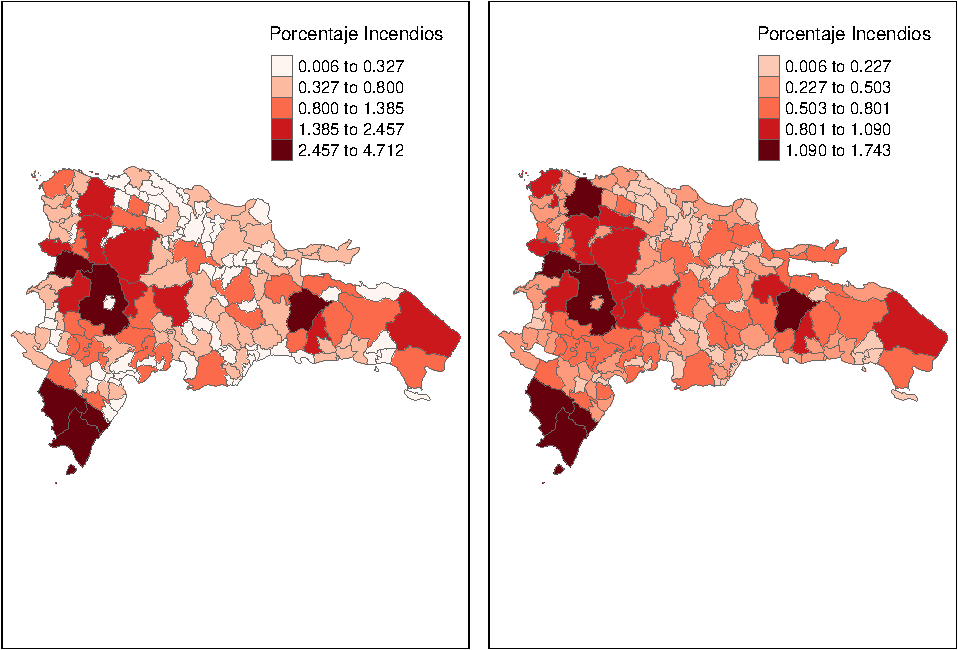
\includegraphics{proyecto_files/figure-latex/unnamed-chunk-21-1.pdf}

Al realizar las pruebas de ``Shapiro-Wilk'' para las columnas
\emph{Porcentaje de Incendios}, \emph{Log Porcentaje de Incendios} y
\emph{Tukey Porcentaje de Incendios} se observa que tan solo la ultima
tiene valores p mayores a 0.05 por lo que no permite su rechazo y se
considera el supuesto de normalidad. Al realizar la prueba
``Breusch-Pagan'' para cada una de estas todas las variables tienen
resultados que pueden ser interpretados con una hipotesis nula que no
puede ser rechazada y con presunción de homocedastisidad esto debido a
que todas superan el p mayor a 0.05.

\begin{Shaded}
\begin{Highlighting}[]
\CommentTok{#qq }
\KeywordTok{qqnorm}\NormalTok{(munIncPerc}\OperatorTok{$}\NormalTok{IncPercentage)}
\end{Highlighting}
\end{Shaded}

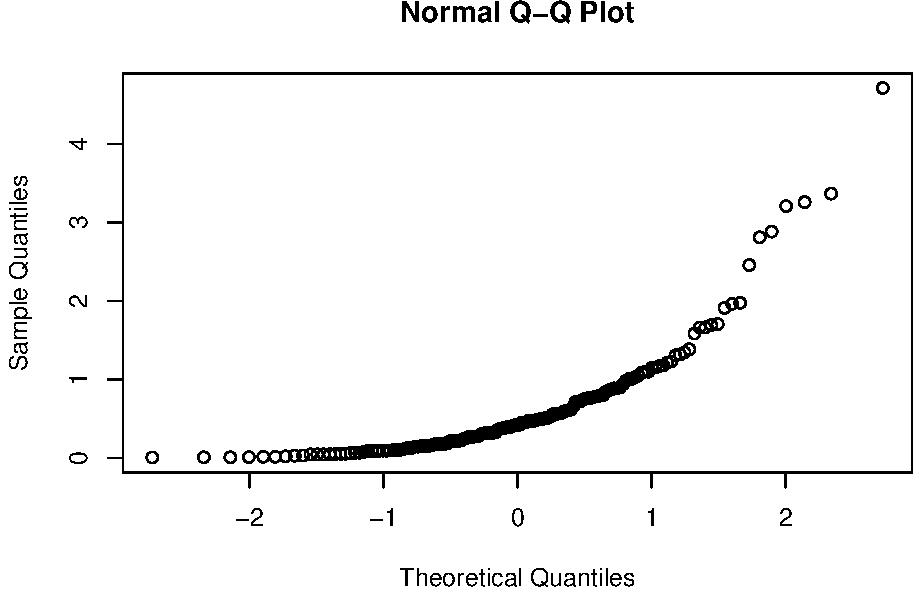
\includegraphics{proyecto_files/figure-latex/unnamed-chunk-22-1.pdf}

\begin{Shaded}
\begin{Highlighting}[]
\KeywordTok{shapiro.test}\NormalTok{(munIncPerc}\OperatorTok{$}\NormalTok{IncPercentage)}
\end{Highlighting}
\end{Shaded}

\begin{verbatim}
## 
##  Shapiro-Wilk normality test
## 
## data:  munIncPerc$IncPercentage
## W = 0.74127, p-value = 3.202e-15
\end{verbatim}

\begin{Shaded}
\begin{Highlighting}[]
\KeywordTok{qqnorm}\NormalTok{(munIncPerc}\OperatorTok{$}\NormalTok{IncPercentage_log)}
\end{Highlighting}
\end{Shaded}

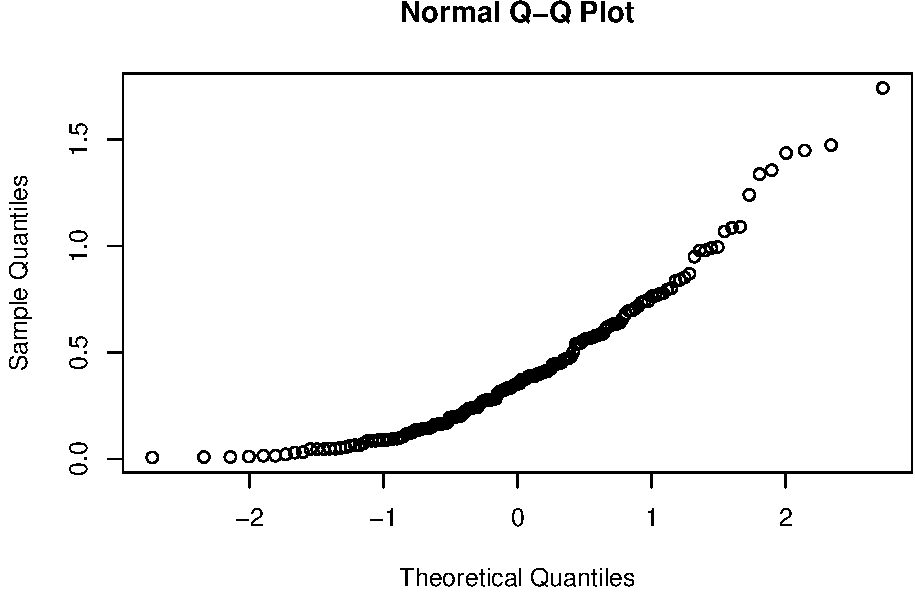
\includegraphics{proyecto_files/figure-latex/unnamed-chunk-22-2.pdf}

\begin{Shaded}
\begin{Highlighting}[]
\KeywordTok{shapiro.test}\NormalTok{(munIncPerc}\OperatorTok{$}\NormalTok{IncPercentage_log)}
\end{Highlighting}
\end{Shaded}

\begin{verbatim}
## 
##  Shapiro-Wilk normality test
## 
## data:  munIncPerc$IncPercentage_log
## W = 0.89833, p-value = 6.953e-09
\end{verbatim}

\begin{Shaded}
\begin{Highlighting}[]
\KeywordTok{qqnorm}\NormalTok{(munIncPerc}\OperatorTok{$}\NormalTok{IncPercentage_tukey)}
\end{Highlighting}
\end{Shaded}

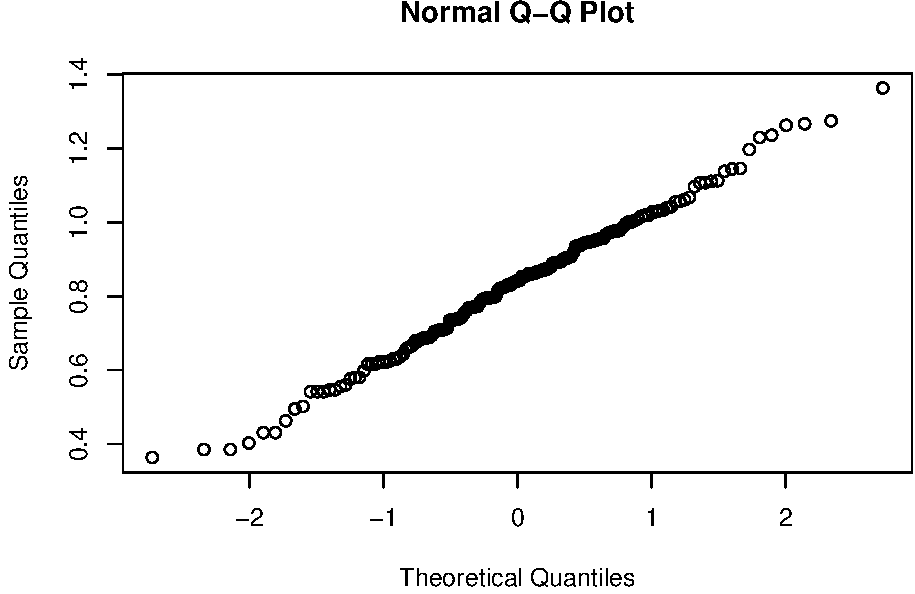
\includegraphics{proyecto_files/figure-latex/unnamed-chunk-22-3.pdf}

\begin{Shaded}
\begin{Highlighting}[]
\KeywordTok{shapiro.test}\NormalTok{(munIncPerc}\OperatorTok{$}\NormalTok{IncPercentage_tukey)}
\end{Highlighting}
\end{Shaded}

\begin{verbatim}
## 
##  Shapiro-Wilk normality test
## 
## data:  munIncPerc$IncPercentage_tukey
## W = 0.99441, p-value = 0.8194
\end{verbatim}

\begin{Shaded}
\begin{Highlighting}[]
\NormalTok{munIncPerc }\OperatorTok\StringTok{ }\KeywordTok{lm}\NormalTok{(IncPercentage }\OperatorTok{~}\StringTok{ }\NormalTok{x, .) }\OperatorTok\StringTok{ }\KeywordTok{bptest}\NormalTok{()}
\end{Highlighting}
\end{Shaded}

\begin{verbatim}
## 
##  studentized Breusch-Pagan test
## 
## data:  .
## BP = 1.6534, df = 1, p-value = 0.1985
\end{verbatim}

\begin{Shaded}
\begin{Highlighting}[]
\NormalTok{munIncPerc }\OperatorTok\StringTok{ }\KeywordTok{lm}\NormalTok{(IncPercentage }\OperatorTok{~}\StringTok{ }\NormalTok{y, .) }\OperatorTok\StringTok{ }\KeywordTok{bptest}\NormalTok{()}
\end{Highlighting}
\end{Shaded}

\begin{verbatim}
## 
##  studentized Breusch-Pagan test
## 
## data:  .
## BP = 1.1426, df = 1, p-value = 0.2851
\end{verbatim}

\begin{Shaded}
\begin{Highlighting}[]
\NormalTok{munIncPerc }\OperatorTok\StringTok{ }\KeywordTok{lm}\NormalTok{(IncPercentage_log }\OperatorTok{~}\StringTok{ }\NormalTok{x, .) }\OperatorTok\StringTok{ }\KeywordTok{bptest}\NormalTok{()}
\end{Highlighting}
\end{Shaded}

\begin{verbatim}
## 
##  studentized Breusch-Pagan test
## 
## data:  .
## BP = 0.61098, df = 1, p-value = 0.4344
\end{verbatim}

\begin{Shaded}
\begin{Highlighting}[]
\NormalTok{munIncPerc }\OperatorTok\StringTok{ }\KeywordTok{lm}\NormalTok{(IncPercentage_log }\OperatorTok{~}\StringTok{ }\NormalTok{y, .) }\OperatorTok\StringTok{ }\KeywordTok{bptest}\NormalTok{()}
\end{Highlighting}
\end{Shaded}

\begin{verbatim}
## 
##  studentized Breusch-Pagan test
## 
## data:  .
## BP = 1.3799, df = 1, p-value = 0.2401
\end{verbatim}

\begin{Shaded}
\begin{Highlighting}[]
\NormalTok{munIncPerc }\OperatorTok\StringTok{ }\KeywordTok{lm}\NormalTok{(IncPercentage_tukey }\OperatorTok{~}\StringTok{ }\NormalTok{x, .) }\OperatorTok\StringTok{ }\KeywordTok{bptest}\NormalTok{()}
\end{Highlighting}
\end{Shaded}

\begin{verbatim}
## 
##  studentized Breusch-Pagan test
## 
## data:  .
## BP = 0.40819, df = 1, p-value = 0.5229
\end{verbatim}

\begin{Shaded}
\begin{Highlighting}[]
\NormalTok{munIncPerc }\OperatorTok\StringTok{ }\KeywordTok{lm}\NormalTok{(IncPercentage_tukey }\OperatorTok{~}\StringTok{ }\NormalTok{y, .) }\OperatorTok\StringTok{ }\KeywordTok{bptest}\NormalTok{()}
\end{Highlighting}
\end{Shaded}

\begin{verbatim}
## 
##  studentized Breusch-Pagan test
## 
## data:  .
## BP = 0.08262, df = 1, p-value = 0.7738
\end{verbatim}

Teniendo en cuenta los resultados anteriores, se evalua la
\emph{autocorrelación espacial global} teniendo en cuenta la prueba para
la ``I'' de Moran usando los pesos estandarizados y los binarios para la
variable de \emph{Tukey} estableciendo que las comprobaciónes son
menores al alpha estipulado permitiendo afirmar al estudio que existe
una autocorrelación espacial.

\begin{Shaded}
\begin{Highlighting}[]
\NormalTok{(gmoranw <-}\StringTok{ }\KeywordTok{moran.test}\NormalTok{(}\DataTypeTok{x =}\NormalTok{ munIncPerc}\OperatorTok{$}\NormalTok{IncXArea_tukey, }\DataTypeTok{listw =}\NormalTok{ munInc.w.W ))}
\end{Highlighting}
\end{Shaded}

\begin{verbatim}
## 
##  Moran I test under randomisation
## 
## data:  munIncPerc$IncXArea_tukey  
## weights: munInc.w.W    
## 
## Moran I statistic standard deviate = 8.6616, p-value < 2.2e-16
## alternative hypothesis: greater
## sample estimates:
## Moran I statistic       Expectation          Variance 
##       0.439964128      -0.006493506       0.002656854
\end{verbatim}

\begin{Shaded}
\begin{Highlighting}[]
\NormalTok{(gmoranb <-}\StringTok{ }\KeywordTok{moran.test}\NormalTok{(}\DataTypeTok{x =}\NormalTok{ munIncPerc}\OperatorTok{$}\NormalTok{IncXArea_tukey, }\DataTypeTok{listw =}\NormalTok{ munInc.w.B))}
\end{Highlighting}
\end{Shaded}

\begin{verbatim}
## 
##  Moran I test under randomisation
## 
## data:  munIncPerc$IncXArea_tukey  
## weights: munInc.w.B    
## 
## Moran I statistic standard deviate = 8.9868, p-value < 2.2e-16
## alternative hypothesis: greater
## sample estimates:
## Moran I statistic       Expectation          Variance 
##       0.431838654      -0.006493506       0.002379007
\end{verbatim}

\begin{Shaded}
\begin{Highlighting}[]
\KeywordTok{moran.plot}\NormalTok{(}\DataTypeTok{x =}\NormalTok{ munIncPerc}\OperatorTok{$}\NormalTok{IncPercentage_tukey, }\DataTypeTok{listw =}\NormalTok{ munInc.w.W)}
\end{Highlighting}
\end{Shaded}

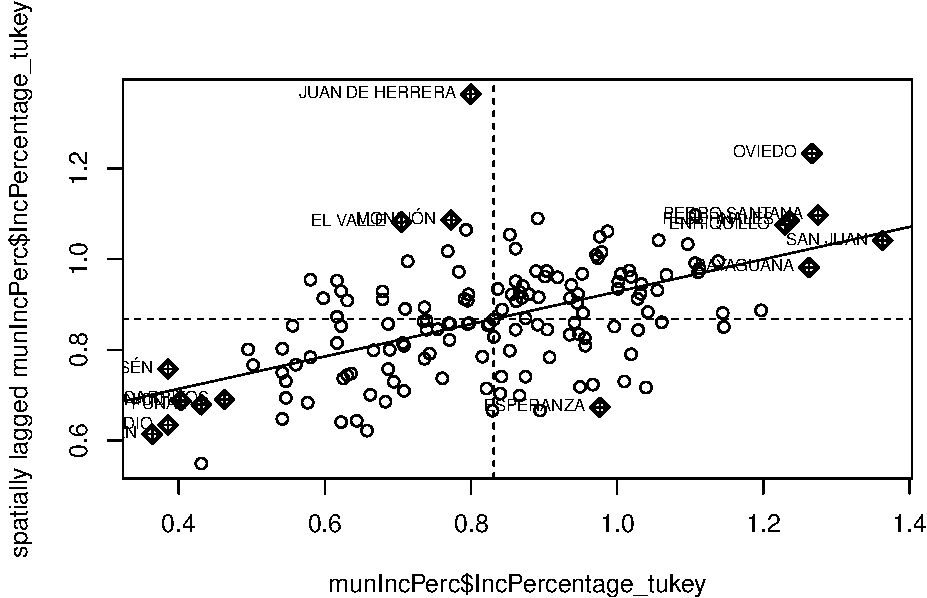
\includegraphics{proyecto_files/figure-latex/unnamed-chunk-23-1.pdf}

Finalmente se realiza el mapa de LISA Cluster para la variable
\emph{Porcentaje de incendios Tukey} arrojando el siguiente resultado
que permite observar que los municipios con correlación espacial para
los incendios son San Juan, Higuey y Neiba.

\begin{verbatim}
## $grafico
\end{verbatim}

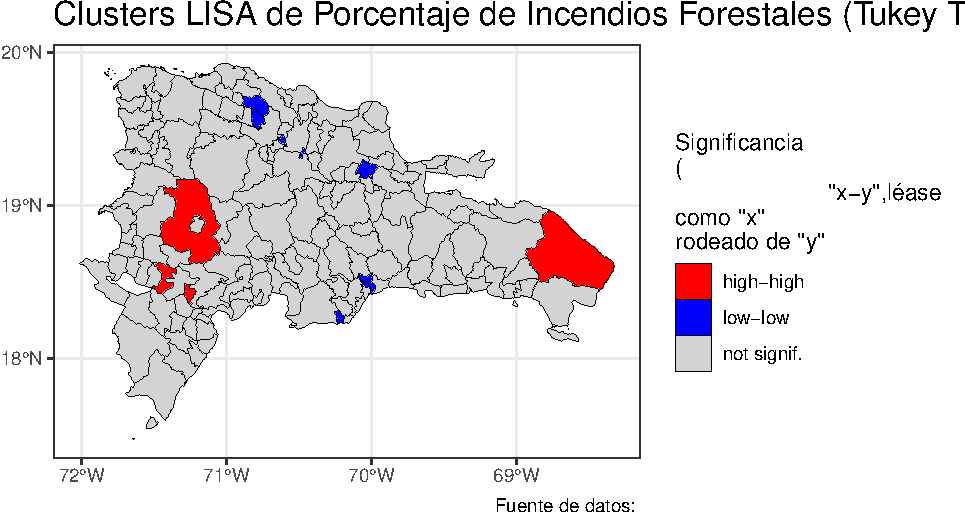
\includegraphics{proyecto_files/figure-latex/unnamed-chunk-24-1.pdf}

\begin{verbatim}
## 
## $objeto
## Simple feature collection with 155 features and 20 fields
## geometry type:  MULTIPOLYGON
## dimension:      XY
## bbox:           xmin: -72.01147 ymin: 17.47033 xmax: -68.32354 ymax: 19.93211
## epsg (SRID):    4326
## proj4string:    +proj=longlat +datum=WGS84 +no_defs
## First 10 features:
##    PROV MUN REG               TOPONIMIA ENLACE NumIncendios IncPercentage
## 1    01  01  10 SANTO DOMINGO DE GUZMÁN 100101            3   0.006364562
## 2    02  01  05                    AZUA 050201          518   1.098947726
## 3    02  02  05             LAS CHARCAS 050202           68   0.144263408
## 4    02  03  05    LAS YAYAS DE VIAJAMA 050203          412   0.874066531
## 5    02  04  05         PADRE LAS CASAS 050204          621   1.317464358
## 6    02  05  05                 PERALTA 050205          262   0.555838425
## 7    02  06  05            SABANA YEGUA 050206           72   0.152749491
## 8    02  07  05            PUEBLO VIEJO 050207           25   0.053038018
## 9    02  08  05           TÁBARA ARRIBA 050208          462   0.980142566
## 10   02  09  05                GUAYABAL 050209          369   0.782841141
##    IncPercentage_log IncPercentage_tukey IncPercentage_tukey_lambda
## 1        0.006344394           0.3637087                        0.2
## 2        0.741436136           1.0190498                        0.2
## 3        0.134761118           0.6789398                        0.2
## 4        0.628110685           0.9734394                        0.2
## 5        0.840473639           1.0566904                        0.2
## 6        0.442014580           0.8891801                        0.2
## 7        0.142149950           0.6867457                        0.2
## 8        0.051679337           0.5557986                        0.2
## 9        0.683168845           0.9959966                        0.2
## 10       0.578208238           0.9522144                        0.2
##      AreaKm2   IncXArea IncXArea_log IncXArea_tukey IncXArea_tukey_lambda
## 1   91.49644 0.03278816    0.0322621      0.3586866                   0.3
## 2  416.24047 1.24447292    0.8084707      1.0678141                   0.3
## 3  246.53555 0.27582229    0.2435909      0.6794990                   0.3
## 4  430.81968 0.95631656    0.6710634      0.9866895                   0.3
## 5  573.56072 1.08271013    0.7336700      1.0241266                   0.3
## 6  129.35998 2.02535594    1.1070288      1.2358063                   0.3
## 7  113.90367 0.63211309    0.4898756      0.8714419                   0.3
## 8   48.08024 0.51996408    0.4186867      0.8218489                   0.3
## 9  274.86478 1.68082650    0.9861251      1.1685757                   0.3
## 10 235.34938 1.56788174    0.9430813      1.1444425                   0.3
##            x        y                       geometry puntuacionz
## 1  -69.94175 18.48488 MULTIPOLYGON (((-69.89794 1...  -2.3235747
## 2  -70.80988 18.42093 MULTIPOLYGON (((-70.71457 1...   0.9344148
## 3  -70.54611 18.39184 MULTIPOLYGON (((-70.50185 1...  -0.7564222
## 4  -70.99966 18.60405 MULTIPOLYGON (((-70.85774 1...   0.7076652
## 5  -70.91135 18.80900 MULTIPOLYGON (((-70.77551 1...   1.1215430
## 6  -70.78275 18.60198 MULTIPOLYGON (((-70.73131 1...   0.2887751
## 7  -70.88809 18.41374 MULTIPOLYGON (((-70.83014 1...  -0.7176153
## 8  -70.78029 18.39309 MULTIPOLYGON (((-70.79387 1...  -1.3686111
## 9  -70.91510 18.49605 MULTIPOLYGON (((-70.83352 1...   0.8198072
## 10 -70.76497 18.71745 MULTIPOLYGON (((-70.68664 1...   0.6021464
##    lagpuntuacionz    quad_sig
## 1      0.43036993 not signif.
## 2     -0.76905286 not signif.
## 3      0.20455192 not signif.
## 4     -1.00787376 not signif.
## 5      0.07620910 not signif.
## 6     -0.04071622 not signif.
## 7     -0.16061258 not signif.
## 8      0.42293128 not signif.
## 9     -0.03986659 not signif.
## 10     0.39438601 not signif.
\end{verbatim}

Para efectos del estudio se repite el proceso descrito anteriormente
para las mismas variables sin embargo teniendo en cuenta el ``área'' de
los municipios esto debido a los resultados vistos en el LISA Cluster.

Teniendo en cuenta que los mapas mostrados a continuación se enfocan en
la cantidad de incendios por km2 se puede observar que los municipios
con mayor cantidad de incendios son los municipios fronterizos de
orografía pronunciada.

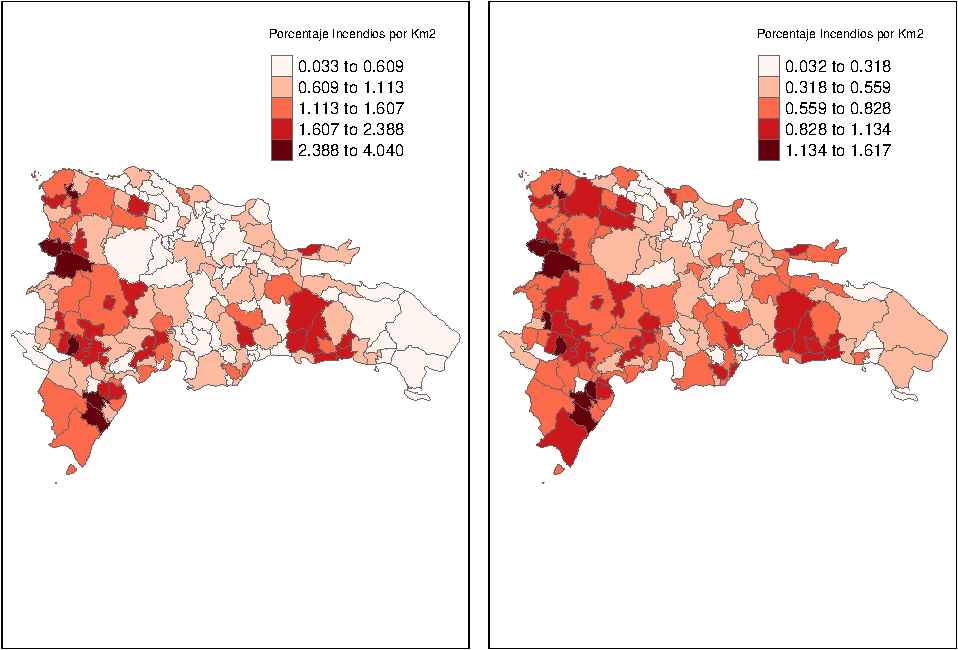
\includegraphics{proyecto_files/figure-latex/unnamed-chunk-26-1.pdf}

Al realizar las pruebas de ``Shapiro-Wilk'' para las columnas
\emph{Porcentaje de Incendios x Area }, \emph{Log Porcentaje de
Incendios x Area} y \emph{Tukey Porcentaje de Incendios x Area} se
observa que tan solo la ultima tiene valores p mayores a 0.05 por lo que
no permite su rechazo y se considera el supuesto de normalidad. Al
realizar la prueba ``Breusch-Pagan'' para cada una de estas todas las
variables tienen resultados que pueden ser interpretados con una
hipotesis nula que no puede ser rechazada y con presunción de
homocedastisidad esto debido a que todas superan el p mayor a 0.05.

\begin{Shaded}
\begin{Highlighting}[]
\CommentTok{#qq }
\KeywordTok{qqnorm}\NormalTok{(munIncPerc}\OperatorTok{$}\NormalTok{IncXArea)}
\end{Highlighting}
\end{Shaded}

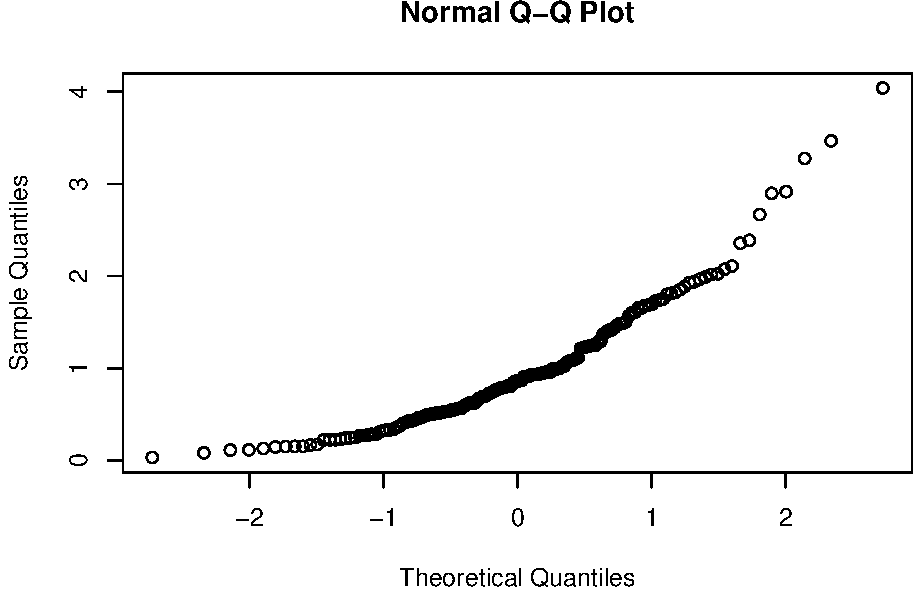
\includegraphics{proyecto_files/figure-latex/unnamed-chunk-27-1.pdf}

\begin{Shaded}
\begin{Highlighting}[]
\KeywordTok{shapiro.test}\NormalTok{(munIncPerc}\OperatorTok{$}\NormalTok{IncXArea)}
\end{Highlighting}
\end{Shaded}

\begin{verbatim}
## 
##  Shapiro-Wilk normality test
## 
## data:  munIncPerc$IncXArea
## W = 0.89846, p-value = 7.076e-09
\end{verbatim}

\begin{Shaded}
\begin{Highlighting}[]
\KeywordTok{qqnorm}\NormalTok{(munIncPerc}\OperatorTok{$}\NormalTok{IncXArea_log)}
\end{Highlighting}
\end{Shaded}

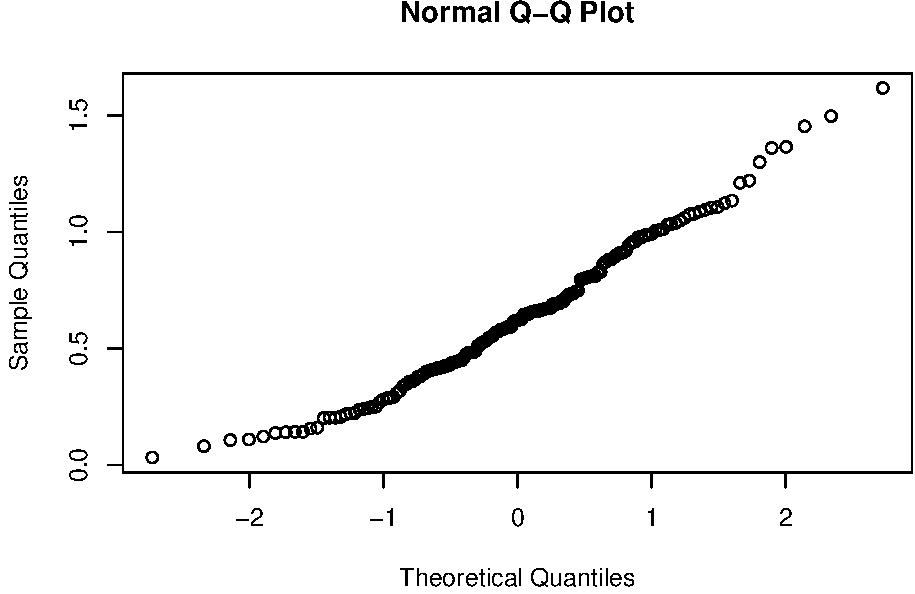
\includegraphics{proyecto_files/figure-latex/unnamed-chunk-27-2.pdf}

\begin{Shaded}
\begin{Highlighting}[]
\KeywordTok{shapiro.test}\NormalTok{(munIncPerc}\OperatorTok{$}\NormalTok{IncXArea_log)}
\end{Highlighting}
\end{Shaded}

\begin{verbatim}
## 
##  Shapiro-Wilk normality test
## 
## data:  munIncPerc$IncXArea_log
## W = 0.9773, p-value = 0.01161
\end{verbatim}

\begin{Shaded}
\begin{Highlighting}[]
\KeywordTok{qqnorm}\NormalTok{(munIncPerc}\OperatorTok{$}\NormalTok{IncXArea_tukey)}
\end{Highlighting}
\end{Shaded}

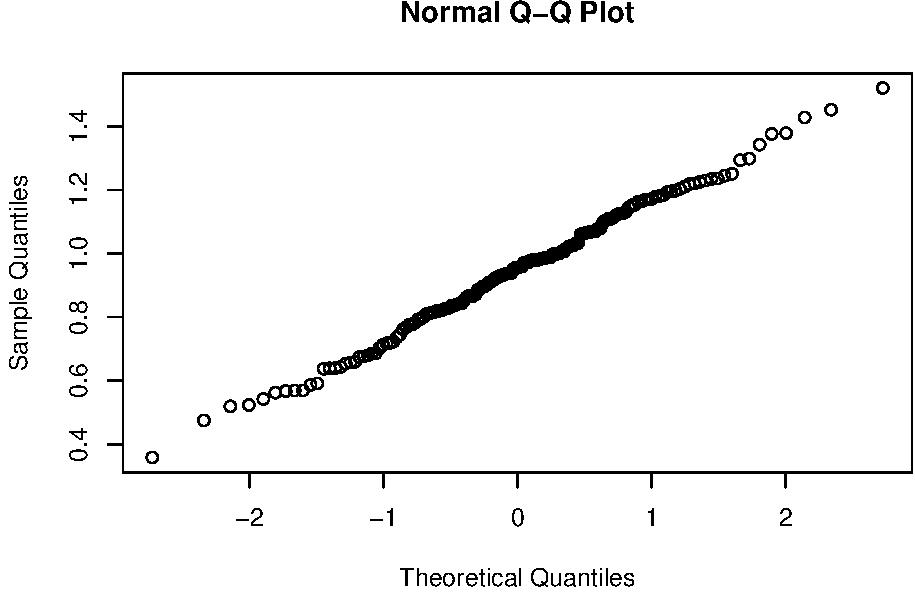
\includegraphics{proyecto_files/figure-latex/unnamed-chunk-27-3.pdf}

\begin{Shaded}
\begin{Highlighting}[]
\KeywordTok{shapiro.test}\NormalTok{(munIncPerc}\OperatorTok{$}\NormalTok{IncXArea_tukey)}
\end{Highlighting}
\end{Shaded}

\begin{verbatim}
## 
##  Shapiro-Wilk normality test
## 
## data:  munIncPerc$IncXArea_tukey
## W = 0.99557, p-value = 0.9253
\end{verbatim}

\begin{Shaded}
\begin{Highlighting}[]
\NormalTok{munIncPerc }\OperatorTok\StringTok{ }\KeywordTok{lm}\NormalTok{(IncXArea }\OperatorTok{~}\StringTok{ }\NormalTok{x, .) }\OperatorTok\StringTok{ }\KeywordTok{bptest}\NormalTok{()}
\end{Highlighting}
\end{Shaded}

\begin{verbatim}
## 
##  studentized Breusch-Pagan test
## 
## data:  .
## BP = 3.3994, df = 1, p-value = 0.06522
\end{verbatim}

\begin{Shaded}
\begin{Highlighting}[]
\NormalTok{munIncPerc }\OperatorTok\StringTok{ }\KeywordTok{lm}\NormalTok{(IncXArea }\OperatorTok{~}\StringTok{ }\NormalTok{y, .) }\OperatorTok\StringTok{ }\KeywordTok{bptest}\NormalTok{()}
\end{Highlighting}
\end{Shaded}

\begin{verbatim}
## 
##  studentized Breusch-Pagan test
## 
## data:  .
## BP = 0.41244, df = 1, p-value = 0.5207
\end{verbatim}

\begin{Shaded}
\begin{Highlighting}[]
\NormalTok{munIncPerc }\OperatorTok\StringTok{ }\KeywordTok{lm}\NormalTok{(IncXArea_log }\OperatorTok{~}\StringTok{ }\NormalTok{x, .) }\OperatorTok\StringTok{ }\KeywordTok{bptest}\NormalTok{()}
\end{Highlighting}
\end{Shaded}

\begin{verbatim}
## 
##  studentized Breusch-Pagan test
## 
## data:  .
## BP = 0.19948, df = 1, p-value = 0.6551
\end{verbatim}

\begin{Shaded}
\begin{Highlighting}[]
\NormalTok{munIncPerc }\OperatorTok\StringTok{ }\KeywordTok{lm}\NormalTok{(IncXArea_log }\OperatorTok{~}\StringTok{ }\NormalTok{y, .) }\OperatorTok\StringTok{ }\KeywordTok{bptest}\NormalTok{()}
\end{Highlighting}
\end{Shaded}

\begin{verbatim}
## 
##  studentized Breusch-Pagan test
## 
## data:  .
## BP = 0.0796, df = 1, p-value = 0.7778
\end{verbatim}

\begin{Shaded}
\begin{Highlighting}[]
\NormalTok{munIncPerc }\OperatorTok\StringTok{ }\KeywordTok{lm}\NormalTok{(IncXArea_tukey }\OperatorTok{~}\StringTok{ }\NormalTok{x, .) }\OperatorTok\StringTok{ }\KeywordTok{bptest}\NormalTok{()}
\end{Highlighting}
\end{Shaded}

\begin{verbatim}
## 
##  studentized Breusch-Pagan test
## 
## data:  .
## BP = 0.18554, df = 1, p-value = 0.6667
\end{verbatim}

\begin{Shaded}
\begin{Highlighting}[]
\NormalTok{munIncPerc }\OperatorTok\StringTok{ }\KeywordTok{lm}\NormalTok{(IncXArea_tukey }\OperatorTok{~}\StringTok{ }\NormalTok{y, .) }\OperatorTok\StringTok{ }\KeywordTok{bptest}\NormalTok{()}
\end{Highlighting}
\end{Shaded}

\begin{verbatim}
## 
##  studentized Breusch-Pagan test
## 
## data:  .
## BP = 0.66037, df = 1, p-value = 0.4164
\end{verbatim}

Teniendo en cuenta los resultados anteriores, se evalua la
\emph{autocorrelación espacial global} teniendo en cuenta la prueba para
la ``I'' de Moran usando los pesos estandarizados y los binarios para la
variable de \emph{Tukey} estableciendo que las comprobaciónes son
menores al alpha estipulado permitiendo afirmar al estudio que existe
una autocorrelación espacial.

\begin{Shaded}
\begin{Highlighting}[]
\NormalTok{(gmoranw <-}\StringTok{ }\KeywordTok{moran.test}\NormalTok{(}\DataTypeTok{x =}\NormalTok{ munIncPerc}\OperatorTok{$}\NormalTok{IncXArea_tukey, }\DataTypeTok{listw =}\NormalTok{ munInc.w.W ))}
\end{Highlighting}
\end{Shaded}

\begin{verbatim}
## 
##  Moran I test under randomisation
## 
## data:  munIncPerc$IncXArea_tukey  
## weights: munInc.w.W    
## 
## Moran I statistic standard deviate = 8.6616, p-value < 2.2e-16
## alternative hypothesis: greater
## sample estimates:
## Moran I statistic       Expectation          Variance 
##       0.439964128      -0.006493506       0.002656854
\end{verbatim}

\begin{Shaded}
\begin{Highlighting}[]
\NormalTok{(gmoranb <-}\StringTok{ }\KeywordTok{moran.test}\NormalTok{(}\DataTypeTok{x =}\NormalTok{ munIncPerc}\OperatorTok{$}\NormalTok{IncXArea_tukey, }\DataTypeTok{listw =}\NormalTok{ munInc.w.B))}
\end{Highlighting}
\end{Shaded}

\begin{verbatim}
## 
##  Moran I test under randomisation
## 
## data:  munIncPerc$IncXArea_tukey  
## weights: munInc.w.B    
## 
## Moran I statistic standard deviate = 8.9868, p-value < 2.2e-16
## alternative hypothesis: greater
## sample estimates:
## Moran I statistic       Expectation          Variance 
##       0.431838654      -0.006493506       0.002379007
\end{verbatim}

\begin{Shaded}
\begin{Highlighting}[]
\KeywordTok{moran.plot}\NormalTok{(}\DataTypeTok{x =}\NormalTok{ munIncPerc}\OperatorTok{$}\NormalTok{IncPercentage_tukey, }\DataTypeTok{listw =}\NormalTok{ munInc.w.W)}
\end{Highlighting}
\end{Shaded}

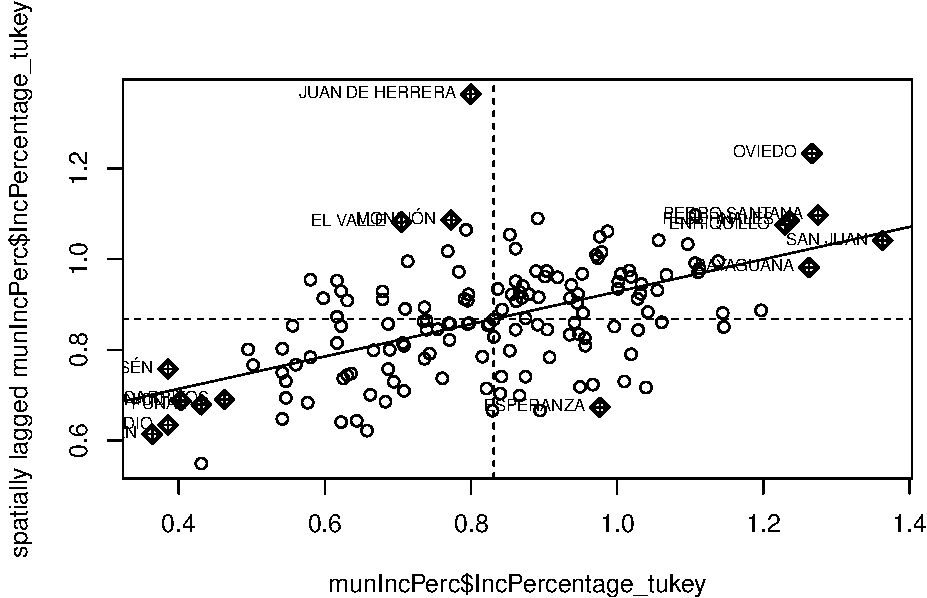
\includegraphics{proyecto_files/figure-latex/unnamed-chunk-28-1.pdf}

Finalmente se realiza el mapa de LISA Cluster para la variable
\emph{Porcentaje de incendios x Area Tukey} arrojando el siguiente
resultado que permite observar que los municipios con correlación
espacial para los incendios teniendo en cuenta su área son Loma de
Cabrera y Polo.

\begin{verbatim}
## $grafico
\end{verbatim}

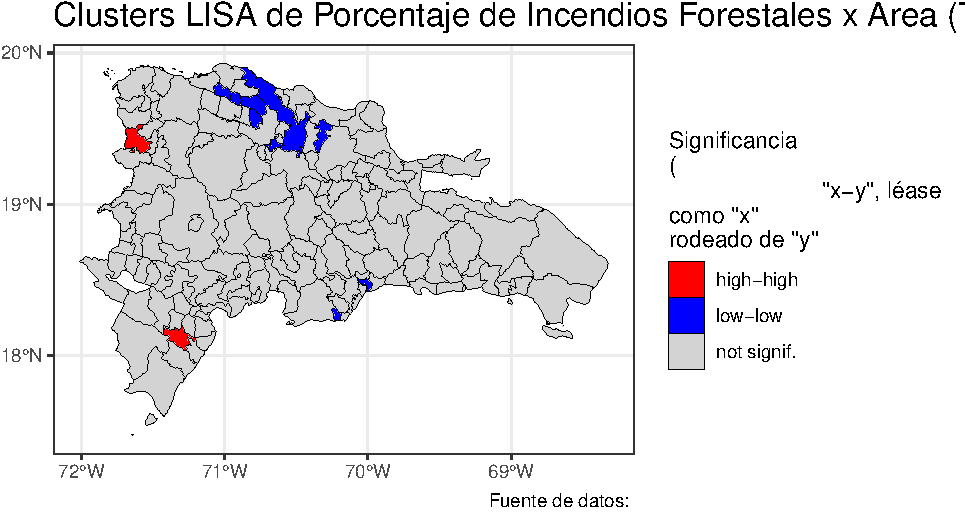
\includegraphics{proyecto_files/figure-latex/unnamed-chunk-29-1.pdf}

\begin{verbatim}
## 
## $objeto
## Simple feature collection with 155 features and 20 fields
## geometry type:  MULTIPOLYGON
## dimension:      XY
## bbox:           xmin: -72.01147 ymin: 17.47033 xmax: -68.32354 ymax: 19.93211
## epsg (SRID):    4326
## proj4string:    +proj=longlat +datum=WGS84 +no_defs
## First 10 features:
##    PROV MUN REG               TOPONIMIA ENLACE NumIncendios IncPercentage
## 1    01  01  10 SANTO DOMINGO DE GUZMÁN 100101            3   0.006364562
## 2    02  01  05                    AZUA 050201          518   1.098947726
## 3    02  02  05             LAS CHARCAS 050202           68   0.144263408
## 4    02  03  05    LAS YAYAS DE VIAJAMA 050203          412   0.874066531
## 5    02  04  05         PADRE LAS CASAS 050204          621   1.317464358
## 6    02  05  05                 PERALTA 050205          262   0.555838425
## 7    02  06  05            SABANA YEGUA 050206           72   0.152749491
## 8    02  07  05            PUEBLO VIEJO 050207           25   0.053038018
## 9    02  08  05           TÁBARA ARRIBA 050208          462   0.980142566
## 10   02  09  05                GUAYABAL 050209          369   0.782841141
##    IncPercentage_log IncPercentage_tukey IncPercentage_tukey_lambda
## 1        0.006344394           0.3637087                        0.2
## 2        0.741436136           1.0190498                        0.2
## 3        0.134761118           0.6789398                        0.2
## 4        0.628110685           0.9734394                        0.2
## 5        0.840473639           1.0566904                        0.2
## 6        0.442014580           0.8891801                        0.2
## 7        0.142149950           0.6867457                        0.2
## 8        0.051679337           0.5557986                        0.2
## 9        0.683168845           0.9959966                        0.2
## 10       0.578208238           0.9522144                        0.2
##      AreaKm2   IncXArea IncXArea_log IncXArea_tukey IncXArea_tukey_lambda
## 1   91.49644 0.03278816    0.0322621      0.3586866                   0.3
## 2  416.24047 1.24447292    0.8084707      1.0678141                   0.3
## 3  246.53555 0.27582229    0.2435909      0.6794990                   0.3
## 4  430.81968 0.95631656    0.6710634      0.9866895                   0.3
## 5  573.56072 1.08271013    0.7336700      1.0241266                   0.3
## 6  129.35998 2.02535594    1.1070288      1.2358063                   0.3
## 7  113.90367 0.63211309    0.4898756      0.8714419                   0.3
## 8   48.08024 0.51996408    0.4186867      0.8218489                   0.3
## 9  274.86478 1.68082650    0.9861251      1.1685757                   0.3
## 10 235.34938 1.56788174    0.9430813      1.1444425                   0.3
##            x        y                       geometry puntuacionz
## 1  -69.94175 18.48488 MULTIPOLYGON (((-69.89794 1...  -2.6897115
## 2  -70.80988 18.42093 MULTIPOLYGON (((-70.71457 1...   0.5638173
## 3  -70.54611 18.39184 MULTIPOLYGON (((-70.50185 1...  -1.2178007
## 4  -70.99966 18.60405 MULTIPOLYGON (((-70.85774 1...   0.1916118
## 5  -70.91135 18.80900 MULTIPOLYGON (((-70.77551 1...   0.3633762
## 6  -70.78275 18.60198 MULTIPOLYGON (((-70.73131 1...   1.3345780
## 7  -70.88809 18.41374 MULTIPOLYGON (((-70.83014 1...  -0.3371526
## 8  -70.78029 18.39309 MULTIPOLYGON (((-70.79387 1...  -0.5646887
## 9  -70.91510 18.49605 MULTIPOLYGON (((-70.83352 1...   1.0261192
## 10 -70.76497 18.71745 MULTIPOLYGON (((-70.68664 1...   0.9153943
##    lagpuntuacionz    quad_sig
## 1      0.56769173 not signif.
## 2     -0.17377395 not signif.
## 3      0.03623403 not signif.
## 4     -1.24703680 not signif.
## 5      0.34551910 not signif.
## 6      0.28475890 not signif.
## 7      0.48035889 not signif.
## 8      0.66046303 not signif.
## 9      0.19931002 not signif.
## 10     0.52734478 not signif.
\end{verbatim}

\subsection{correlación variables world
clim}\label{correlaciuxf3n-variables-world-clim}

Para la segunda parte de esta investigación, se añaden las variables de
Version2 (2000) \emph{Precipitación} \emph{Viento} \emph{Temperatura
Promedio} y \emph{Radiación Solar}, a la información de los Incendios
Forestales asi como las columnas de \emph{mes}, \emph{año} y \emph{Id
unico}. Cabe notar que la data de ``WorldClim'' se establece basandose
un promedio mensual en el periodo 1970-2000

\section{* Stack}\label{stack}

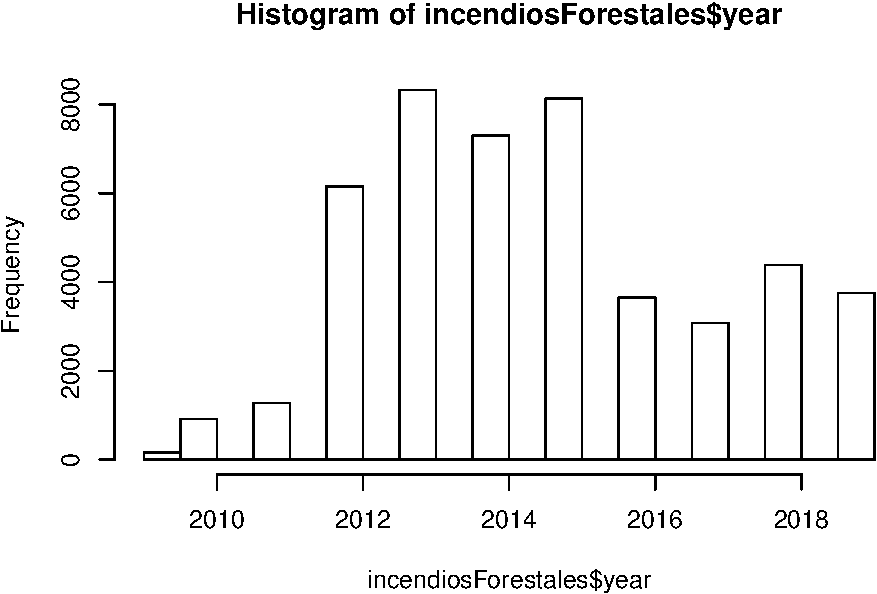
\includegraphics{proyecto_files/figure-latex/unnamed-chunk-30-1.pdf}

Martínez Batlle (2019b) realizó el script de adición de data basandose
en la localización del incendio y el mes de adquisición por parte de la
NASA por cada una de las variables a estudiar dando como resultado el
archivo
\texttt{puntos\_calor\_fuegos\_y\_worldclim\_viento\_temp\_radiacion}.
Sin embargo este script necesita de una unidad de computo de altas
prestaciones por lo que es recomendable no realizar dicho procedimiento
en equipos con menos de 64Gb de memoria RAM y multiples cores para su
procesamiento.

Para efectos prácticos, se realizó el mismo procedimiento usando la
herramienta QGis mediante el \texttt{plugin\ point\ sampling\ tool}
estableciendo el valor de todas las variables climaticas para cada
incendio, el \emph{mes} y \emph{ID unico} obteniendo una tabla que fue
exportada con formato ``CSV''. La misma se abre en el software
``Openoffice Calc'' y por medio la funcion ``Buscar'' para la matriz
estableciendo el valor para cada incendio tomando en cuenta el valor del
mes.

Con el resultado anterior se realiza un \emph{left join} con la tabla
inicial de incendios forestales usando como punto de enlace el valor
``ID Unico'' Posteriormente se quitan los valores que obtuvieron como
valor 0 debido a que estos son errores puesto que se conoce que en el
país no existe ese valor para ninguna de las variables.

Teniendo en cuenta el siguiente gráfico se decide un valor promedio de
basandose en el año, puesto que el manejo de todos los datos se torna
complicado con una máquina con prestaciones insuficientes ademas para
poder realizar las pruebas ``Saphiro-Wilk'' las cuales no se pueden
realizar con mas de 5000 datos.

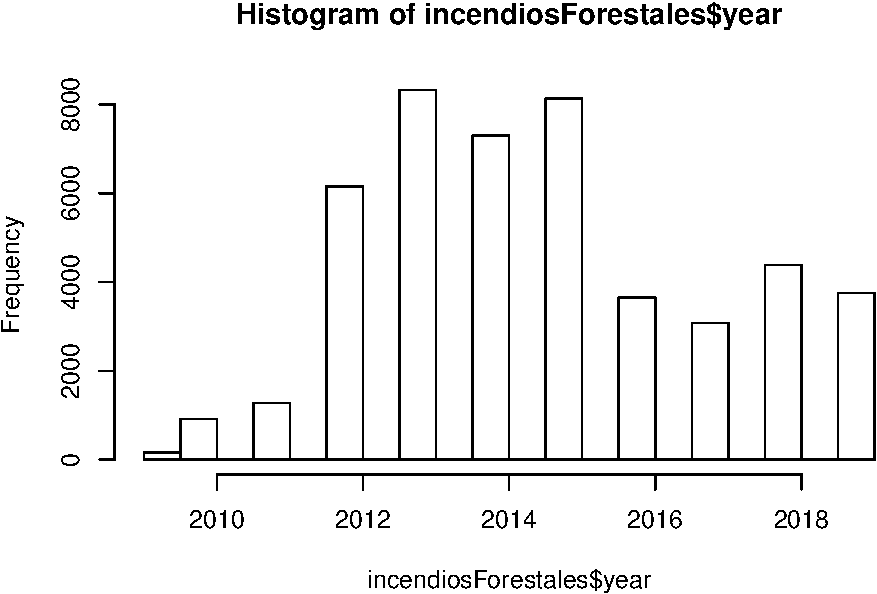
\includegraphics{proyecto_files/figure-latex/unnamed-chunk-33-1.pdf}
Basandose en lo descrito anteriormente y se establece el 2018 como el
año con el que se puede realizar una mejor estimación ademas cuenta con
4374 datos.

Se obtienen los datos estadísticos para el añó 2018

\begin{Shaded}
\begin{Highlighting}[]
\CommentTok{#Año 2018}
\CommentTok{#EDA}
\KeywordTok{nrow}\NormalTok{(incForWC2018)}
\end{Highlighting}
\end{Shaded}

\begin{verbatim}
## [1] 4374
\end{verbatim}

\begin{Shaded}
\begin{Highlighting}[]
\KeywordTok{summary}\NormalTok{(incForWC2018}\OperatorTok{$}\NormalTok{prec)}
\end{Highlighting}
\end{Shaded}

\begin{verbatim}
##    Min. 1st Qu.  Median    Mean 3rd Qu.    Max. 
##   11.00   55.00   89.00   95.05  129.00  298.00
\end{verbatim}

\begin{Shaded}
\begin{Highlighting}[]
\KeywordTok{summary}\NormalTok{(incForWC2018}\OperatorTok{$}\NormalTok{wind)}
\end{Highlighting}
\end{Shaded}

\begin{verbatim}
##    Min. 1st Qu.  Median    Mean 3rd Qu.    Max. 
##   1.304   2.100   2.460   2.625   3.088   4.600
\end{verbatim}

\begin{Shaded}
\begin{Highlighting}[]
\KeywordTok{summary}\NormalTok{(incForWC2018}\OperatorTok{$}\NormalTok{srad)}
\end{Highlighting}
\end{Shaded}

\begin{verbatim}
##    Min. 1st Qu.  Median    Mean 3rd Qu.    Max. 
##   12794   18651   20113   19446   20914   22359
\end{verbatim}

\begin{Shaded}
\begin{Highlighting}[]
\KeywordTok{summary}\NormalTok{(incForWC2018}\OperatorTok{$}\NormalTok{temp)}
\end{Highlighting}
\end{Shaded}

\begin{verbatim}
##    Min. 1st Qu.  Median    Mean 3rd Qu.    Max. 
##   11.33   22.72   24.90   24.34   26.65   29.42
\end{verbatim}

Se realiza la prueba ``Shapiro-Wilk'' para las cuatro variables y su
logaritmo sin embargo se puede observar que ninguna pasa la prueba
puesta que ninguna supera el valor de 0.05, sin embargo se realiza un
ploteo informativo de la variable basado en la localización de los
incendios.

\begin{Shaded}
\begin{Highlighting}[]
\CommentTok{#Temperatura}
\KeywordTok{hist}\NormalTok{(incForWC2018}\OperatorTok{$}\NormalTok{prec)}
\end{Highlighting}
\end{Shaded}

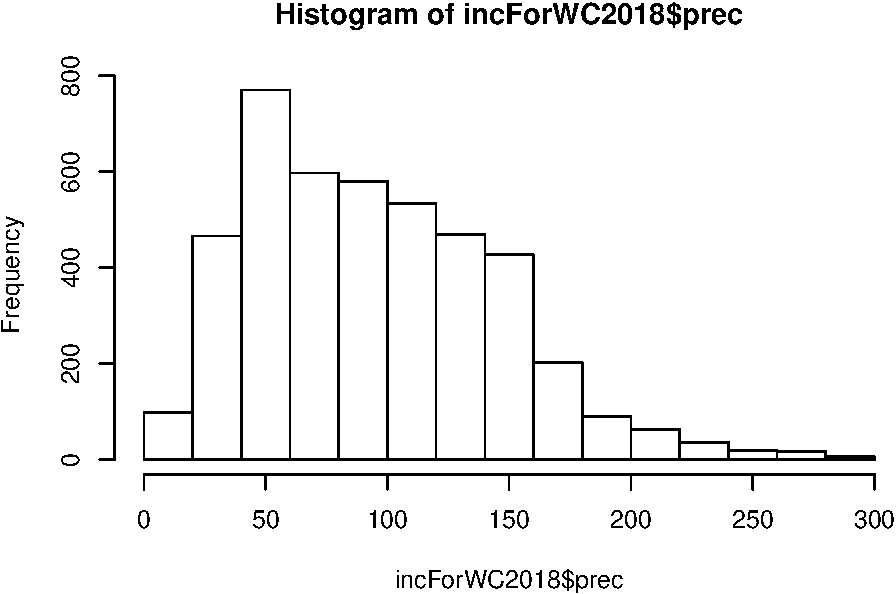
\includegraphics{proyecto_files/figure-latex/unnamed-chunk-36-1.pdf}

\begin{Shaded}
\begin{Highlighting}[]
\KeywordTok{shapiro.test}\NormalTok{(incForWC2018}\OperatorTok{$}\NormalTok{temp)}
\end{Highlighting}
\end{Shaded}

\begin{verbatim}
## 
##  Shapiro-Wilk normality test
## 
## data:  incForWC2018$temp
## W = 0.93385, p-value < 2.2e-16
\end{verbatim}

\begin{Shaded}
\begin{Highlighting}[]
\KeywordTok{shapiro.test}\NormalTok{(}\KeywordTok{log}\NormalTok{(incForWC2018}\OperatorTok{$}\NormalTok{temp))}
\end{Highlighting}
\end{Shaded}

\begin{verbatim}
## 
##  Shapiro-Wilk normality test
## 
## data:  log(incForWC2018$temp)
## W = 0.89088, p-value < 2.2e-16
\end{verbatim}

\begin{Shaded}
\begin{Highlighting}[]
\KeywordTok{ggplot}\NormalTok{() }\OperatorTok{+}
\StringTok{  }\KeywordTok{geom_sf}\NormalTok{(}\DataTypeTok{data =}\NormalTok{ mun4326, }\DataTypeTok{fill =} \StringTok{'white'}\NormalTok{) }\OperatorTok{+}
\StringTok{  }\KeywordTok{geom_sf}\NormalTok{(}\DataTypeTok{data =}\NormalTok{ incForWC2018, }\KeywordTok{aes}\NormalTok{(}\DataTypeTok{col =}\NormalTok{ temp), }\DataTypeTok{size =} \DecValTok{3}\NormalTok{) }\OperatorTok{+}
\StringTok{  }\KeywordTok{scale_colour_gradient}\NormalTok{(}\DataTypeTok{low=}\StringTok{"#f7dede"}\NormalTok{, }\DataTypeTok{high=}\StringTok{"#ff0011"}\NormalTok{) }\OperatorTok{+}
\StringTok{  }\KeywordTok{geom_sf_text}\NormalTok{(}\DataTypeTok{data =}\NormalTok{ incForWC2018, }\KeywordTok{aes}\NormalTok{(}\DataTypeTok{label=}\NormalTok{MUN), }
               \DataTypeTok{check_overlap =}\NormalTok{ T, }\DataTypeTok{size =} \FloatTok{0.5}\NormalTok{) }\OperatorTok{+}
\StringTok{  }\KeywordTok{theme_bw}\NormalTok{()}
\end{Highlighting}
\end{Shaded}

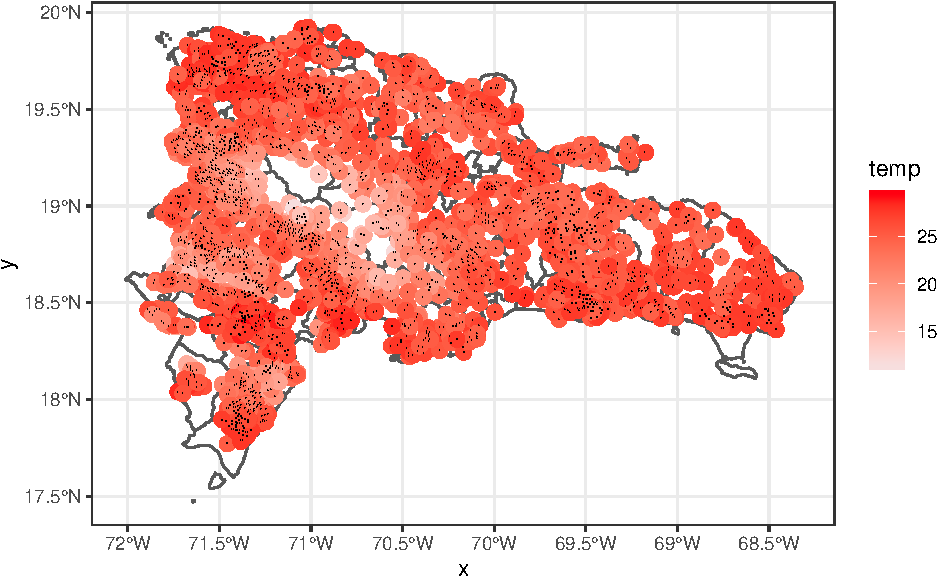
\includegraphics{proyecto_files/figure-latex/unnamed-chunk-36-2.pdf}

\begin{Shaded}
\begin{Highlighting}[]
\CommentTok{#Radiacion Solar}
\KeywordTok{shapiro.test}\NormalTok{(incForWC2018}\OperatorTok{$}\NormalTok{srad)}
\end{Highlighting}
\end{Shaded}

\begin{verbatim}
## 
##  Shapiro-Wilk normality test
## 
## data:  incForWC2018$srad
## W = 0.82435, p-value < 2.2e-16
\end{verbatim}

\begin{Shaded}
\begin{Highlighting}[]
\KeywordTok{shapiro.test}\NormalTok{(}\KeywordTok{log}\NormalTok{(incForWC2018}\OperatorTok{$}\NormalTok{srad))}
\end{Highlighting}
\end{Shaded}

\begin{verbatim}
## 
##  Shapiro-Wilk normality test
## 
## data:  log(incForWC2018$srad)
## W = 0.78429, p-value < 2.2e-16
\end{verbatim}

\begin{Shaded}
\begin{Highlighting}[]
\KeywordTok{ggplot}\NormalTok{() }\OperatorTok{+}
\StringTok{  }\KeywordTok{geom_sf}\NormalTok{(}\DataTypeTok{data =}\NormalTok{ mun4326, }\DataTypeTok{fill =} \StringTok{'white'}\NormalTok{) }\OperatorTok{+}
\StringTok{  }\KeywordTok{geom_sf}\NormalTok{(}\DataTypeTok{data =}\NormalTok{ incForWC2018, }\KeywordTok{aes}\NormalTok{(}\DataTypeTok{col =}\NormalTok{ srad), }\DataTypeTok{size =} \DecValTok{3}\NormalTok{) }\OperatorTok{+}
\StringTok{  }\KeywordTok{scale_colour_gradient}\NormalTok{(}\DataTypeTok{low=}\StringTok{"#f7dede"}\NormalTok{, }\DataTypeTok{high=}\StringTok{"#ff0011"}\NormalTok{) }\OperatorTok{+}
\StringTok{  }\KeywordTok{geom_sf_text}\NormalTok{(}\DataTypeTok{data =}\NormalTok{ incForWC2018, }\KeywordTok{aes}\NormalTok{(}\DataTypeTok{label=}\NormalTok{MUN),}
               \DataTypeTok{check_overlap =}\NormalTok{ T, }\DataTypeTok{size =} \FloatTok{0.5}\NormalTok{) }\OperatorTok{+}
\StringTok{  }\KeywordTok{theme_bw}\NormalTok{()}
\end{Highlighting}
\end{Shaded}

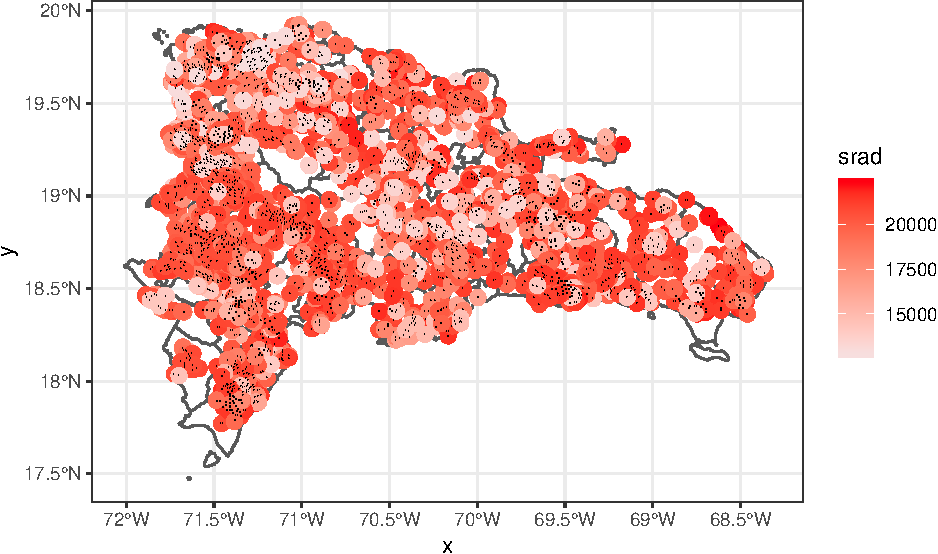
\includegraphics{proyecto_files/figure-latex/unnamed-chunk-36-3.pdf}

\begin{Shaded}
\begin{Highlighting}[]
\CommentTok{#Viento}
\KeywordTok{shapiro.test}\NormalTok{(incForWC2018}\OperatorTok{$}\NormalTok{wind)}
\end{Highlighting}
\end{Shaded}

\begin{verbatim}
## 
##  Shapiro-Wilk normality test
## 
## data:  incForWC2018$wind
## W = 0.94401, p-value < 2.2e-16
\end{verbatim}

\begin{Shaded}
\begin{Highlighting}[]
\KeywordTok{shapiro.test}\NormalTok{(}\KeywordTok{log}\NormalTok{(incForWC2018}\OperatorTok{$}\NormalTok{wind))}
\end{Highlighting}
\end{Shaded}

\begin{verbatim}
## 
##  Shapiro-Wilk normality test
## 
## data:  log(incForWC2018$wind)
## W = 0.97691, p-value < 2.2e-16
\end{verbatim}

\begin{Shaded}
\begin{Highlighting}[]
\KeywordTok{ggplot}\NormalTok{() }\OperatorTok{+}
\StringTok{  }\KeywordTok{geom_sf}\NormalTok{(}\DataTypeTok{data =}\NormalTok{ mun4326, }\DataTypeTok{fill =} \StringTok{'white'}\NormalTok{) }\OperatorTok{+}
\StringTok{  }\KeywordTok{geom_sf}\NormalTok{(}\DataTypeTok{data =}\NormalTok{ incForWC2018, }\KeywordTok{aes}\NormalTok{(}\DataTypeTok{col =}\NormalTok{ wind), }\DataTypeTok{size =} \DecValTok{3}\NormalTok{) }\OperatorTok{+}
\StringTok{  }\KeywordTok{scale_colour_gradient}\NormalTok{(}\DataTypeTok{low=}\StringTok{"#deebf7"}\NormalTok{, }\DataTypeTok{high=}\StringTok{"#3182bd"}\NormalTok{) }\OperatorTok{+}
\StringTok{  }\KeywordTok{geom_sf_text}\NormalTok{(}\DataTypeTok{data =}\NormalTok{ incForWC2018, }\KeywordTok{aes}\NormalTok{(}\DataTypeTok{label=}\NormalTok{MUN), }
               \DataTypeTok{check_overlap =}\NormalTok{ T, }\DataTypeTok{size =} \FloatTok{0.5}\NormalTok{) }\OperatorTok{+}
\StringTok{  }\KeywordTok{theme_bw}\NormalTok{()}
\end{Highlighting}
\end{Shaded}

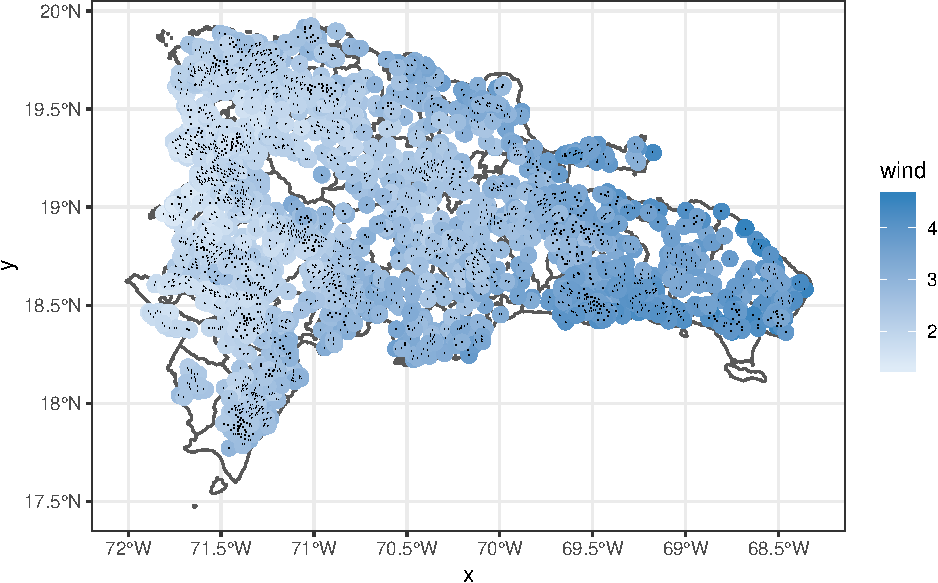
\includegraphics{proyecto_files/figure-latex/unnamed-chunk-36-4.pdf}

\begin{Shaded}
\begin{Highlighting}[]
\CommentTok{#Precipitacion}
\KeywordTok{shapiro.test}\NormalTok{(incForWC2018}\OperatorTok{$}\NormalTok{prec)}
\end{Highlighting}
\end{Shaded}

\begin{verbatim}
## 
##  Shapiro-Wilk normality test
## 
## data:  incForWC2018$prec
## W = 0.95828, p-value < 2.2e-16
\end{verbatim}

\begin{Shaded}
\begin{Highlighting}[]
\KeywordTok{shapiro.test}\NormalTok{(}\KeywordTok{log}\NormalTok{(incForWC2018}\OperatorTok{$}\NormalTok{prec))}
\end{Highlighting}
\end{Shaded}

\begin{verbatim}
## 
##  Shapiro-Wilk normality test
## 
## data:  log(incForWC2018$prec)
## W = 0.97345, p-value < 2.2e-16
\end{verbatim}

\begin{Shaded}
\begin{Highlighting}[]
\KeywordTok{ggplot}\NormalTok{() }\OperatorTok{+}
\StringTok{  }\KeywordTok{geom_sf}\NormalTok{(}\DataTypeTok{data =}\NormalTok{ mun4326, }\DataTypeTok{fill =} \StringTok{'white'}\NormalTok{) }\OperatorTok{+}
\StringTok{  }\KeywordTok{geom_sf}\NormalTok{(}\DataTypeTok{data =}\NormalTok{ incForWC2018, }\KeywordTok{aes}\NormalTok{(}\DataTypeTok{col =}\NormalTok{ prec), }\DataTypeTok{size =} \DecValTok{3}\NormalTok{) }\OperatorTok{+}
\StringTok{  }\KeywordTok{scale_colour_gradient}\NormalTok{(}\DataTypeTok{low=}\StringTok{"#deebf7"}\NormalTok{, }\DataTypeTok{high=}\StringTok{"#3182bd"}\NormalTok{) }\OperatorTok{+}
\StringTok{  }\KeywordTok{geom_sf_text}\NormalTok{(}\DataTypeTok{data =}\NormalTok{ incForWC2018, }\KeywordTok{aes}\NormalTok{(}\DataTypeTok{label=}\NormalTok{MUN),}
               \DataTypeTok{check_overlap =}\NormalTok{ T, }\DataTypeTok{size =} \FloatTok{0.5}\NormalTok{) }\OperatorTok{+}
\StringTok{  }\KeywordTok{theme_bw}\NormalTok{()}
\end{Highlighting}
\end{Shaded}

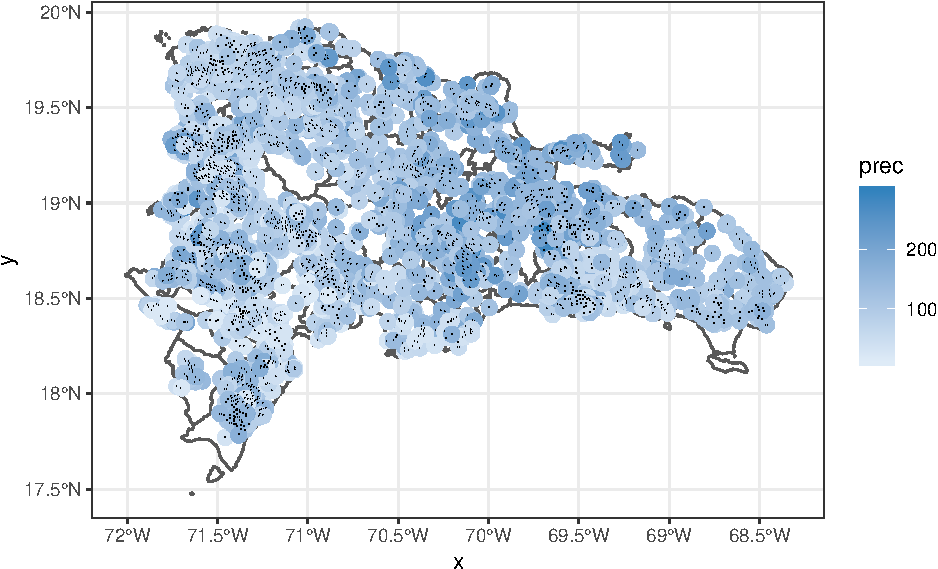
\includegraphics{proyecto_files/figure-latex/unnamed-chunk-36-5.pdf}

Se realiza un variograma del modelo para cada una de las variables y de
esta manera establecer cual podría ser el que se utilizará para el
desarrollo de la interpolación ``krige''. A continuación se detalla para
cada una de las variables.

Radiacion Solar

\begin{Shaded}
\begin{Highlighting}[]
\KeywordTok{plot}\NormalTok{(vsrad18, }\DataTypeTok{plot.numbers =}\NormalTok{ T)}
\end{Highlighting}
\end{Shaded}

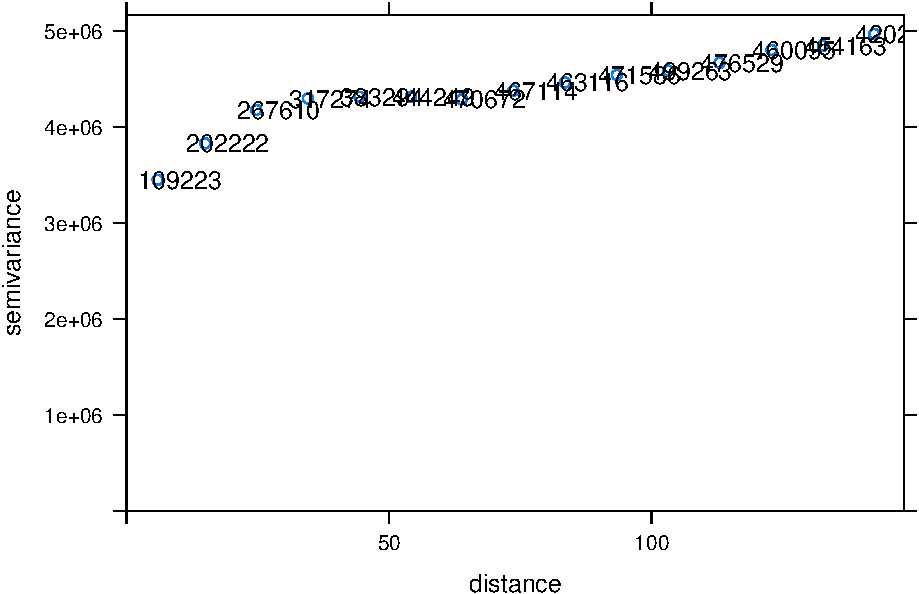
\includegraphics{proyecto_files/figure-latex/unnamed-chunk-38-1.pdf}

\begin{Shaded}
\begin{Highlighting}[]
\NormalTok{vsrad18_m1}
\end{Highlighting}
\end{Shaded}

\begin{verbatim}
##   model   psill    range
## 1   Exp 4186621 3.456893
\end{verbatim}

\begin{Shaded}
\begin{Highlighting}[]
\KeywordTok{plot}\NormalTok{(vsrad18, vsrad18_m1, }\DataTypeTok{plot.numbers =}\NormalTok{ T)}
\end{Highlighting}
\end{Shaded}

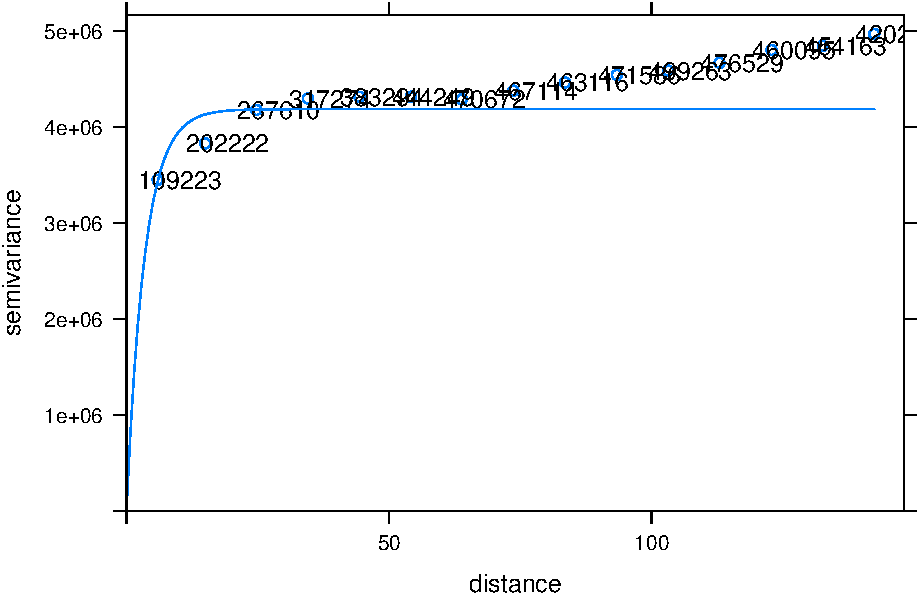
\includegraphics{proyecto_files/figure-latex/unnamed-chunk-38-2.pdf}

Temperatura

\begin{Shaded}
\begin{Highlighting}[]
\KeywordTok{plot}\NormalTok{(vtemp18, }\DataTypeTok{plot.numbers =}\NormalTok{ T)}
\end{Highlighting}
\end{Shaded}

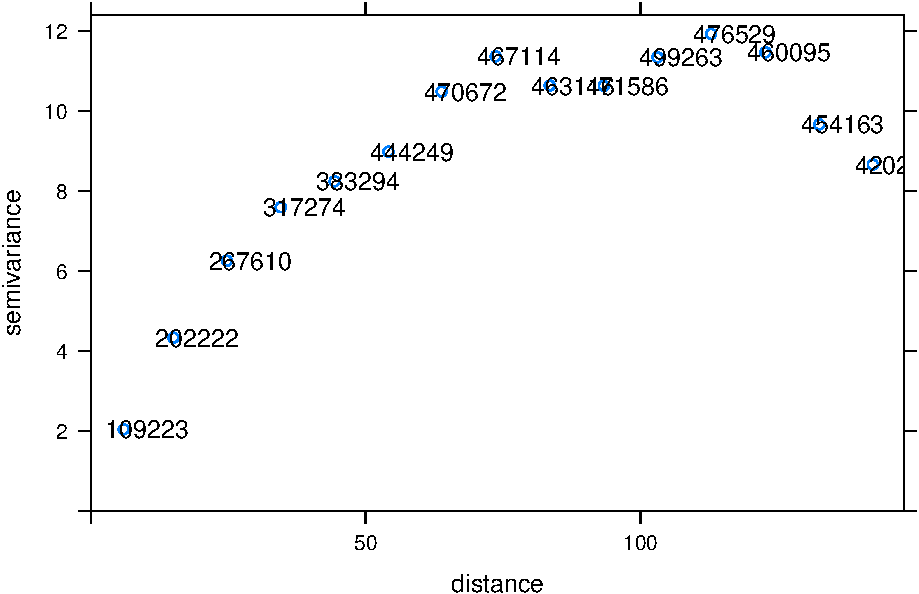
\includegraphics{proyecto_files/figure-latex/unnamed-chunk-40-1.pdf}

\begin{Shaded}
\begin{Highlighting}[]
\NormalTok{vtemp18_m1}
\end{Highlighting}
\end{Shaded}

\begin{verbatim}
##   model    psill    range
## 1   Exp 11.31686 30.64284
\end{verbatim}

\begin{Shaded}
\begin{Highlighting}[]
\KeywordTok{plot}\NormalTok{(vtemp18, vtemp18_m1, }\DataTypeTok{plot.numbers =}\NormalTok{ T)}
\end{Highlighting}
\end{Shaded}

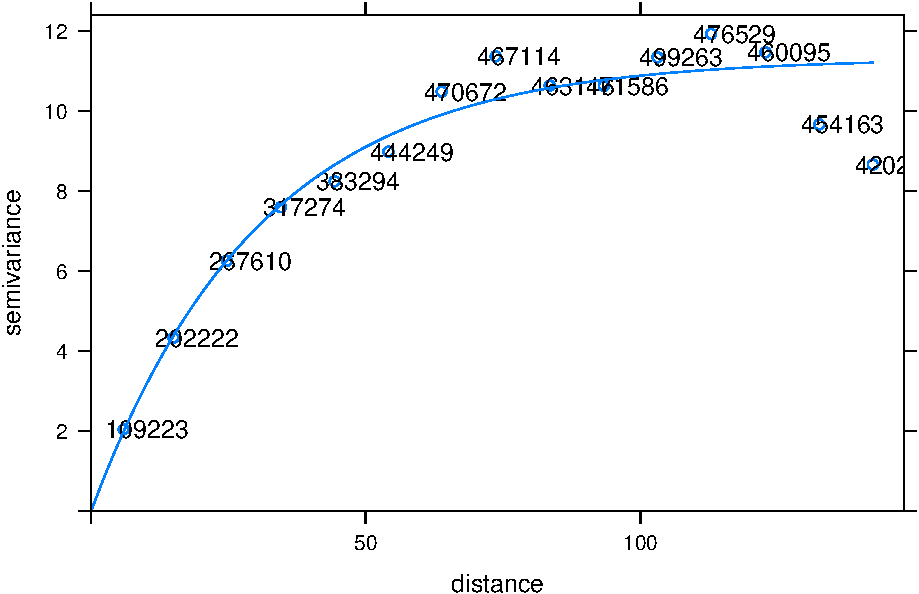
\includegraphics{proyecto_files/figure-latex/unnamed-chunk-40-2.pdf}

\begin{Shaded}
\begin{Highlighting}[]
\KeywordTok{attr}\NormalTok{(vtemp18_m1, }\StringTok{'SSErr'}\NormalTok{)}
\end{Highlighting}
\end{Shaded}

\begin{verbatim}
## [1] 441.3533
\end{verbatim}

Viento

\begin{Shaded}
\begin{Highlighting}[]
\KeywordTok{plot}\NormalTok{(vwind18, }\DataTypeTok{plot.numbers =}\NormalTok{ T)}
\end{Highlighting}
\end{Shaded}

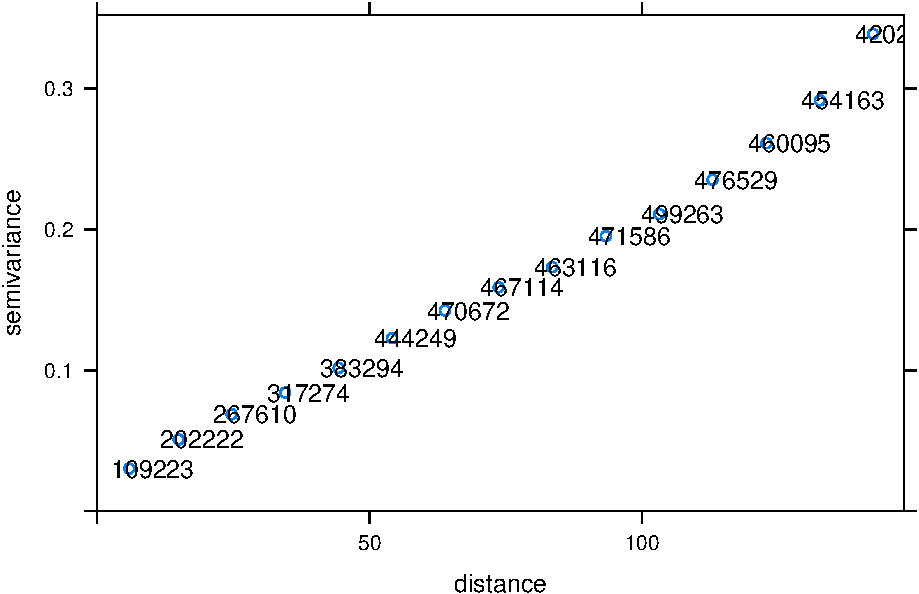
\includegraphics{proyecto_files/figure-latex/unnamed-chunk-42-1.pdf}

\begin{Shaded}
\begin{Highlighting}[]
\NormalTok{vwind18_m1}
\end{Highlighting}
\end{Shaded}

\begin{verbatim}
##   model     psill   range
## 1   Lin 0.3388659 147.004
\end{verbatim}

\begin{Shaded}
\begin{Highlighting}[]
\KeywordTok{plot}\NormalTok{(vwind18, vwind18_m1, }\DataTypeTok{plot.numbers =}\NormalTok{ T)}
\end{Highlighting}
\end{Shaded}

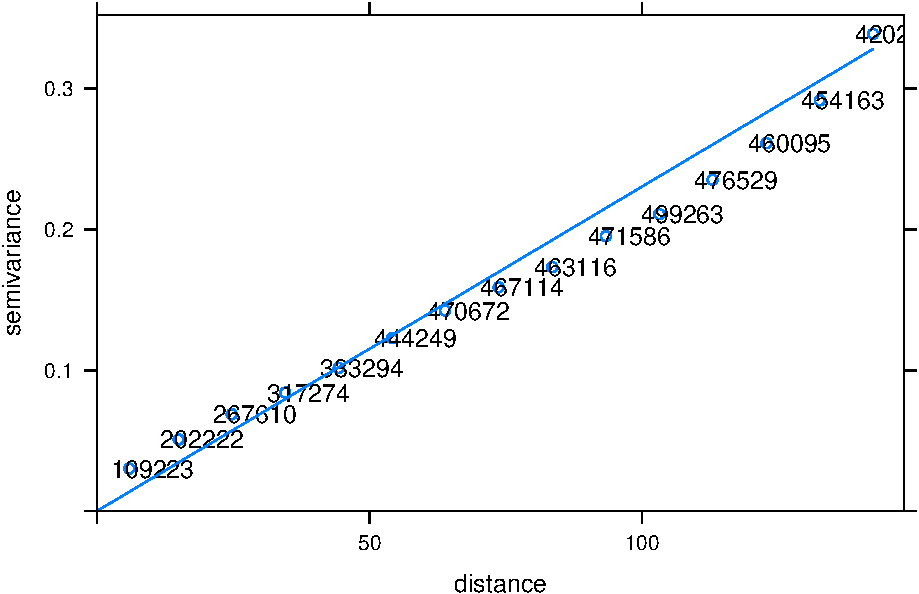
\includegraphics{proyecto_files/figure-latex/unnamed-chunk-42-2.pdf}

\begin{Shaded}
\begin{Highlighting}[]
\NormalTok{vwind18_m2}
\end{Highlighting}
\end{Shaded}

\begin{verbatim}
##   model     psill    range
## 1   Exp 0.3920755 126.1115
\end{verbatim}

\begin{Shaded}
\begin{Highlighting}[]
\KeywordTok{plot}\NormalTok{(vwind18, vwind18_m2, }\DataTypeTok{plot.numbers =}\NormalTok{ T)}
\end{Highlighting}
\end{Shaded}

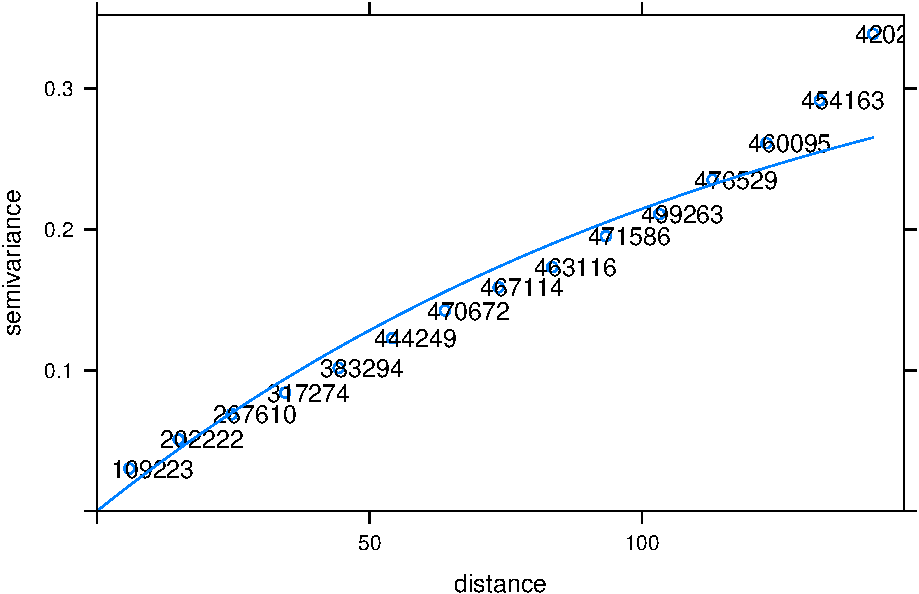
\includegraphics{proyecto_files/figure-latex/unnamed-chunk-42-3.pdf}

\begin{Shaded}
\begin{Highlighting}[]
\NormalTok{vwind18_m3}
\end{Highlighting}
\end{Shaded}

\begin{verbatim}
##   model       psill     range
## 1   Pow 0.006660904 0.7477137
\end{verbatim}

\begin{Shaded}
\begin{Highlighting}[]
\KeywordTok{plot}\NormalTok{(vwind18, vwind18_m3, }\DataTypeTok{plot.numbers =}\NormalTok{ T)}
\end{Highlighting}
\end{Shaded}

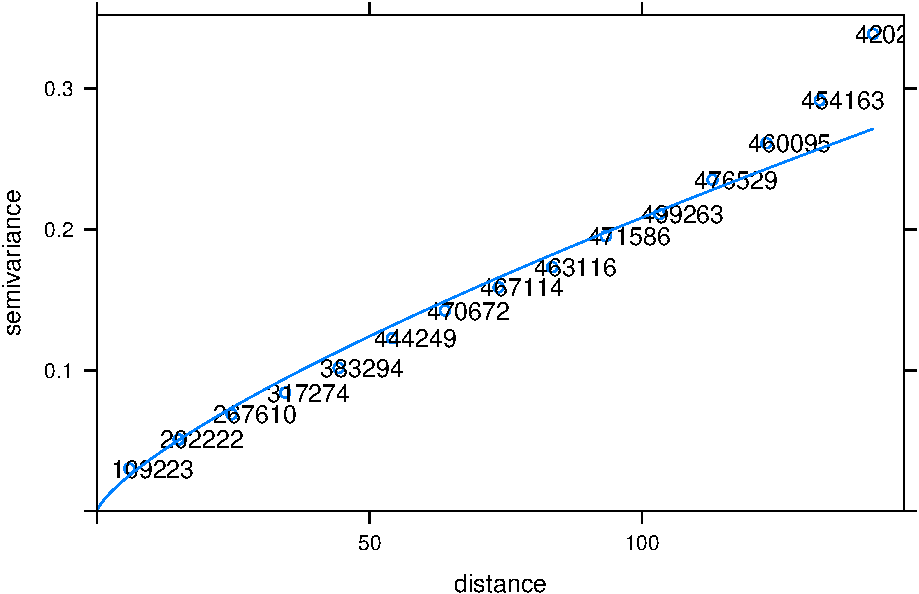
\includegraphics{proyecto_files/figure-latex/unnamed-chunk-42-4.pdf}

\begin{Shaded}
\begin{Highlighting}[]
\KeywordTok{attr}\NormalTok{(vwind18_m1, }\StringTok{'SSErr'}\NormalTok{)}
\end{Highlighting}
\end{Shaded}

\begin{verbatim}
## [1] 1.287008
\end{verbatim}

\begin{Shaded}
\begin{Highlighting}[]
\KeywordTok{attr}\NormalTok{(vwind18_m2, }\StringTok{'SSErr'}\NormalTok{)}
\end{Highlighting}
\end{Shaded}

\begin{verbatim}
## [1] 0.8203171
\end{verbatim}

\begin{Shaded}
\begin{Highlighting}[]
\KeywordTok{attr}\NormalTok{(vwind18_m3, }\StringTok{'SSErr'}\NormalTok{) }\CommentTok{#***}
\end{Highlighting}
\end{Shaded}

\begin{verbatim}
## [1] 0.3033476
\end{verbatim}

Precipitación

\begin{Shaded}
\begin{Highlighting}[]
\KeywordTok{plot}\NormalTok{(vprec18, }\DataTypeTok{plot.numbers =}\NormalTok{ T)}
\end{Highlighting}
\end{Shaded}

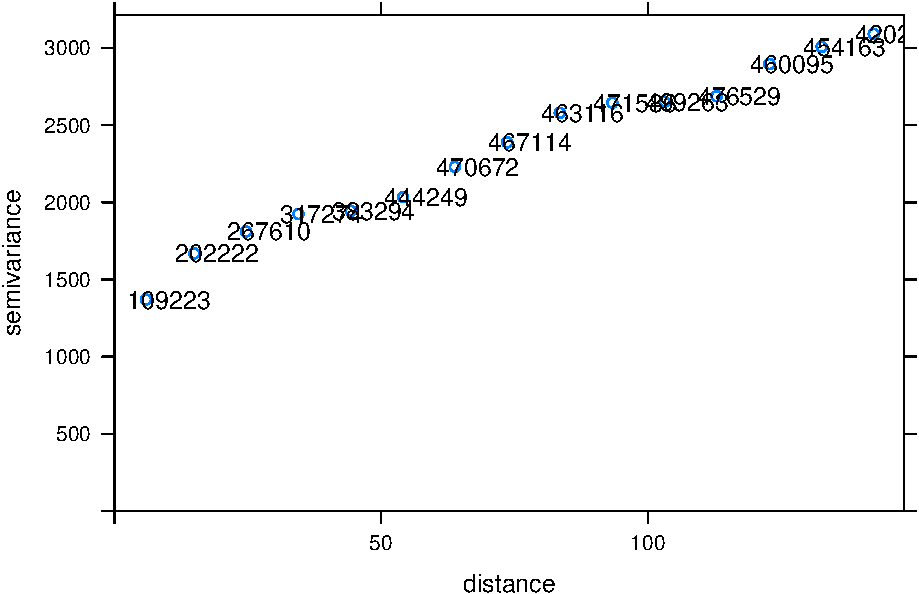
\includegraphics{proyecto_files/figure-latex/unnamed-chunk-44-1.pdf}

\begin{Shaded}
\begin{Highlighting}[]
\NormalTok{vprec18_m1}
\end{Highlighting}
\end{Shaded}

\begin{verbatim}
##   model    psill    range
## 1   Pen 2864.107 4995.939
\end{verbatim}

\begin{Shaded}
\begin{Highlighting}[]
\KeywordTok{plot}\NormalTok{(vprec18, vprec18_m1, }\DataTypeTok{plot.numbers =}\NormalTok{ T)}
\end{Highlighting}
\end{Shaded}

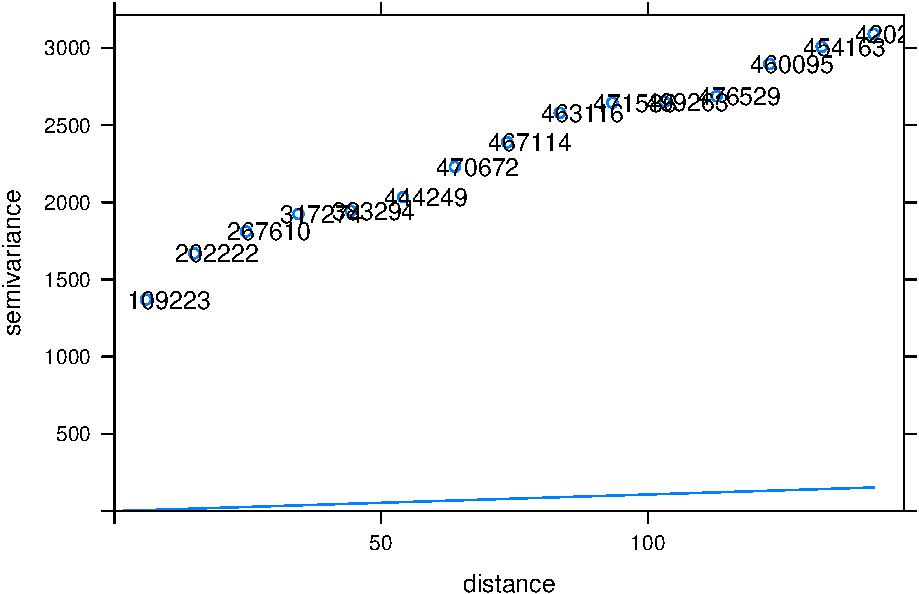
\includegraphics{proyecto_files/figure-latex/unnamed-chunk-44-2.pdf}
Teniendo en cuenta los resultados obtenidos, se visualiza que el modelo
No.3 para el viento basado en el modelo \emph{Pow (power)} es el que da
mejor resultado por lo cual será utilizado para el modelo de
interpolación ``Krige'' para esto se genera una grilla de 10km y se
realiza una transformación a UTM19N:32619 para poder realizar el modelo.

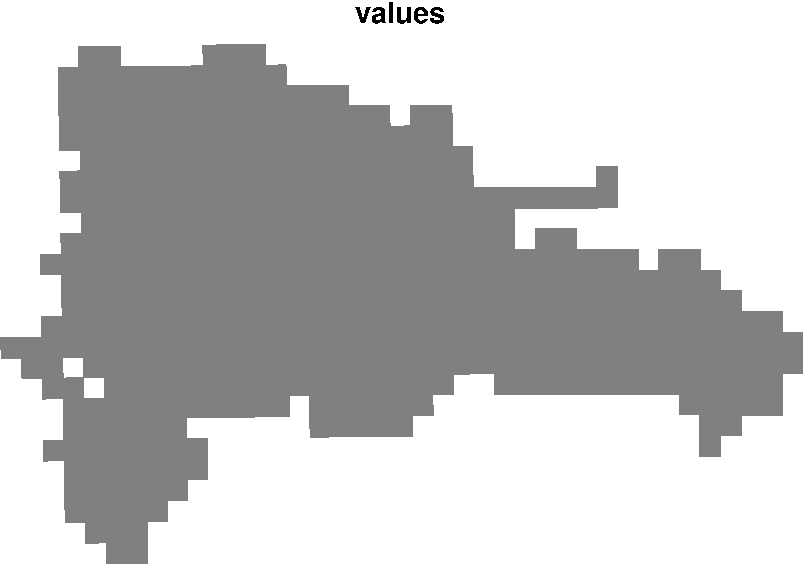
\includegraphics{proyecto_files/figure-latex/unnamed-chunk-45-1.pdf}
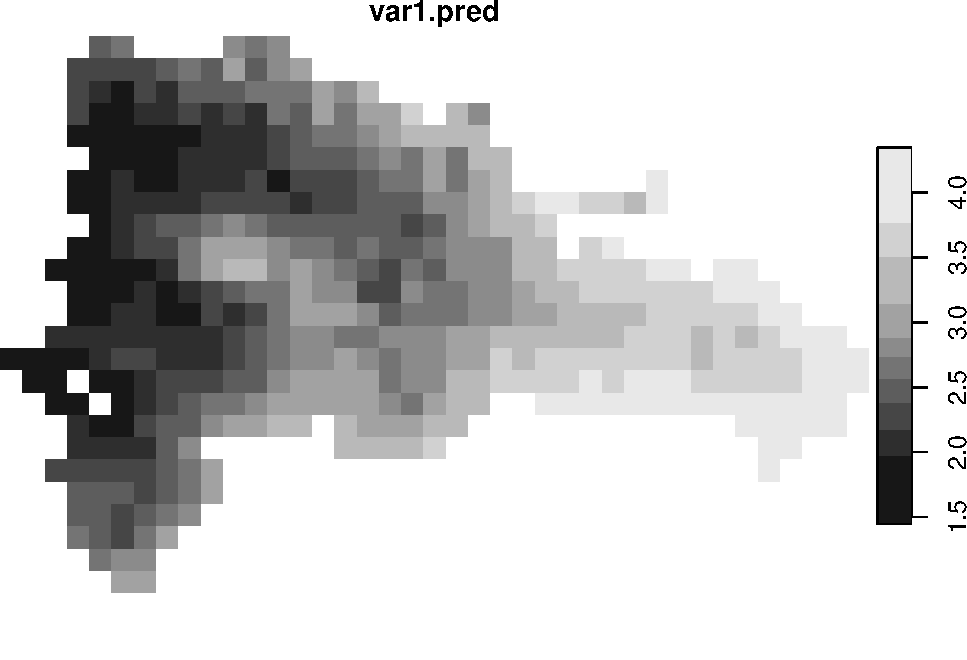
\includegraphics{proyecto_files/figure-latex/unnamed-chunk-46-1.pdf}
Como resultado del modelo ``Krige'' se obtiene el siguiente modelo para
el pais basado en los vientos.
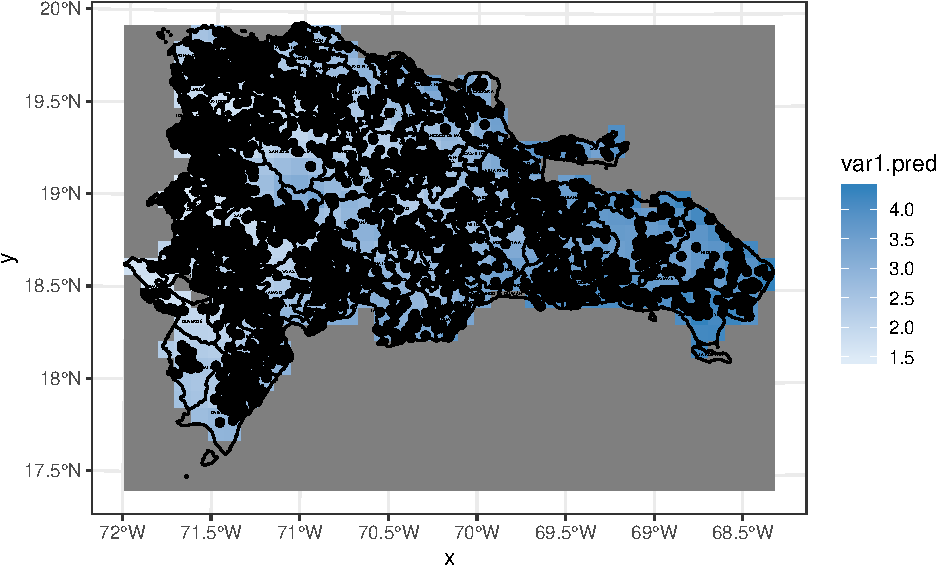
\includegraphics{proyecto_files/figure-latex/unnamed-chunk-47-1.pdf}

Por ultimo se realiza un modelo de predicción teniendo en cuenta el
modelo basandose en un modelo digital de elevaciones para buscar las
zonas mas propensas teniendo en cuenta los incendios y la elevación para
cada uno de los puntos.

Teniendo en cuenta los datos para el numero de incendios se observa que
mediante la modificación de los datos usando un logaritmo se
estandarizan un poco permitiendo realizar un modelo mas cercano a la
realidad.

\begin{Shaded}
\begin{Highlighting}[]
\KeywordTok{hist}\NormalTok{(munIncPerc}\OperatorTok{$}\NormalTok{NumIncendios)}
\end{Highlighting}
\end{Shaded}

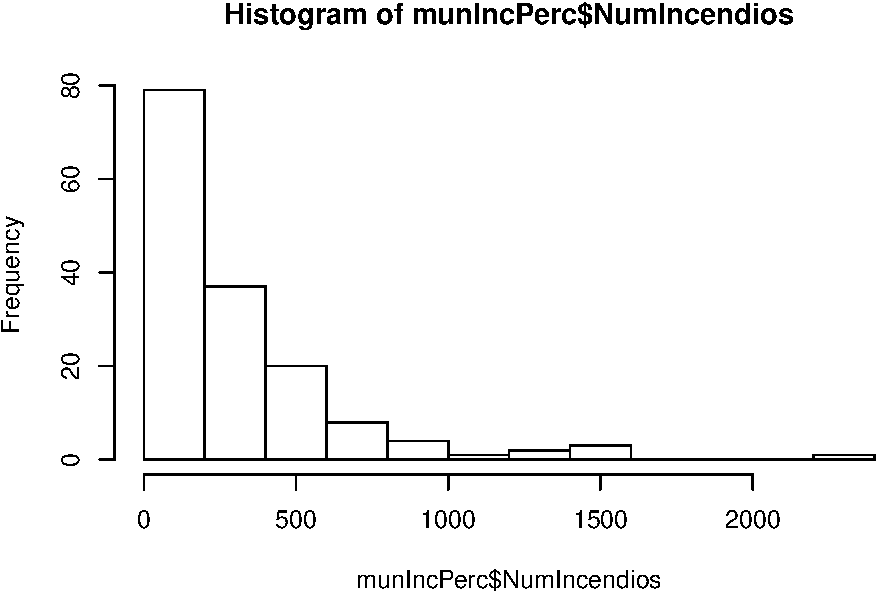
\includegraphics{proyecto_files/figure-latex/unnamed-chunk-49-1.pdf}

\begin{Shaded}
\begin{Highlighting}[]
\KeywordTok{qqnorm}\NormalTok{(munIncPerc}\OperatorTok{$}\NormalTok{NumIncendios)}
\end{Highlighting}
\end{Shaded}

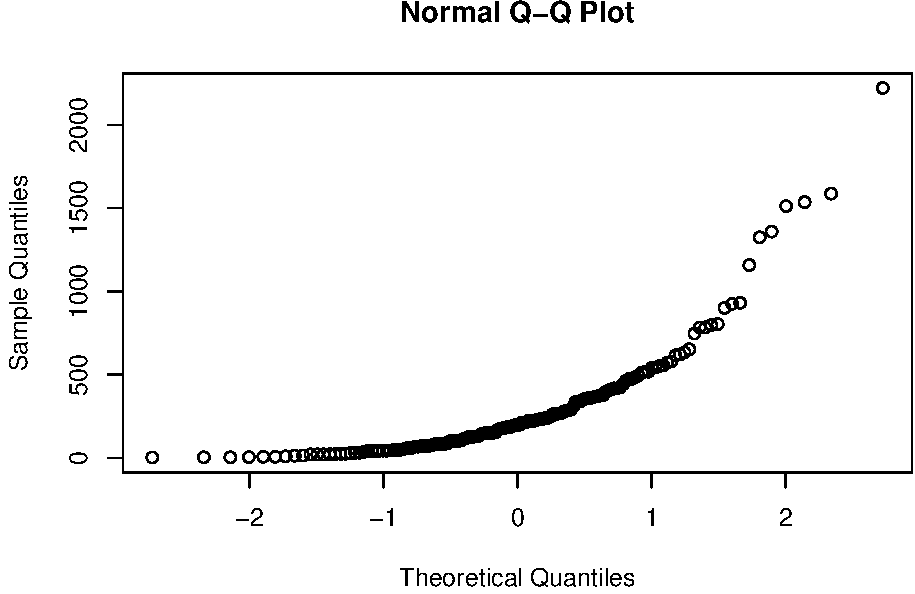
\includegraphics{proyecto_files/figure-latex/unnamed-chunk-49-2.pdf}

\begin{Shaded}
\begin{Highlighting}[]
\KeywordTok{shapiro.test}\NormalTok{(munIncPerc}\OperatorTok{$}\NormalTok{NumIncendios)}
\end{Highlighting}
\end{Shaded}

\begin{verbatim}
## 
##  Shapiro-Wilk normality test
## 
## data:  munIncPerc$NumIncendios
## W = 0.74127, p-value = 3.202e-15
\end{verbatim}

\begin{Shaded}
\begin{Highlighting}[]
\KeywordTok{hist}\NormalTok{(}\KeywordTok{log}\NormalTok{(munIncPerc}\OperatorTok{$}\NormalTok{NumIncendios))}
\end{Highlighting}
\end{Shaded}

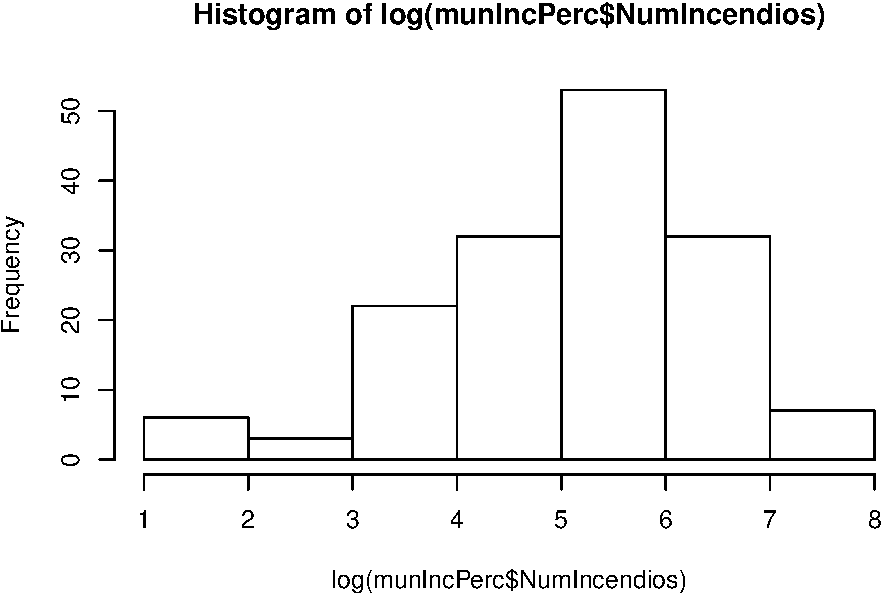
\includegraphics{proyecto_files/figure-latex/unnamed-chunk-49-3.pdf}

\begin{Shaded}
\begin{Highlighting}[]
\KeywordTok{qqnorm}\NormalTok{(}\KeywordTok{log}\NormalTok{(munIncPerc}\OperatorTok{$}\NormalTok{NumIncendios))}
\end{Highlighting}
\end{Shaded}

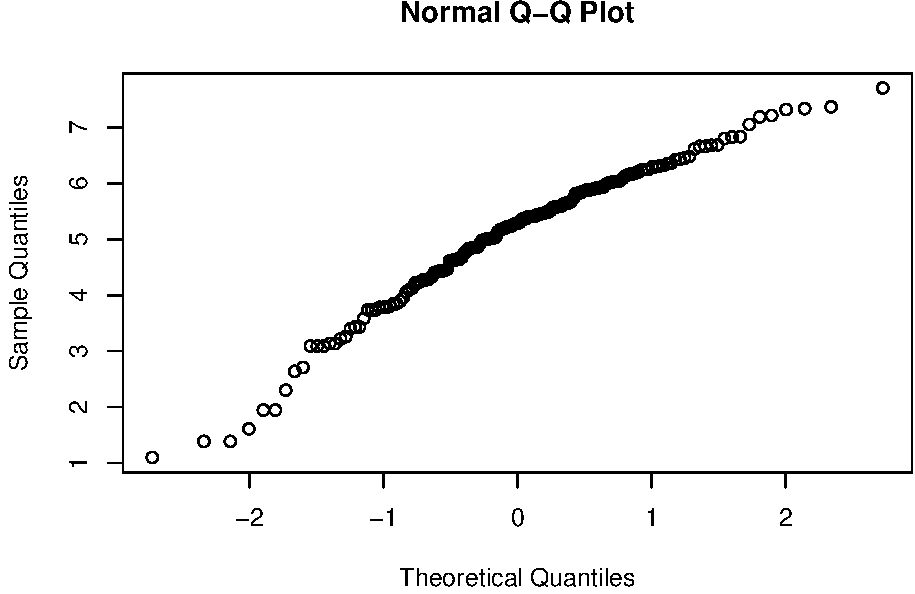
\includegraphics{proyecto_files/figure-latex/unnamed-chunk-49-4.pdf}

\begin{Shaded}
\begin{Highlighting}[]
\KeywordTok{shapiro.test}\NormalTok{(}\KeywordTok{log}\NormalTok{(munIncPerc}\OperatorTok{$}\NormalTok{NumIncendios))}
\end{Highlighting}
\end{Shaded}

\begin{verbatim}
## 
##  Shapiro-Wilk normality test
## 
## data:  log(munIncPerc$NumIncendios)
## W = 0.96419, p-value = 0.0004752
\end{verbatim}

Visto desde un mapa se representa de la siguiente manera
\includegraphics{proyecto_files/figure-latex/unnamed-chunk-50-1.pdf}

Se carga el modelo digital de elevación y se asignan los valores de
elevación para cada incendio, ademas se remuestrea el valor basandose en
la cuadricula de 10km realizada anteriormente, esta misma sirve para
predecir los valores de incendios.

Se observa en el siguiente gráfico que la mayoría de incendios se
presentan en elevaciones menores a 500m.

\includegraphics{proyecto_files/figure-latex/unnamed-chunk-52-1.pdf}

\begin{Shaded}
\begin{Highlighting}[]
\KeywordTok{summary}\NormalTok{(munIncPercGeom_lm)}
\end{Highlighting}
\end{Shaded}

\begin{verbatim}
## 
## Call:
## lm(formula = NumIncendios ~ ele, data = munIncPercGeom)
## 
## Residuals:
##     Min      1Q  Median      3Q     Max 
## -465.17 -213.78  -93.47   97.76 1821.90 
## 
## Coefficients:
##              Estimate Std. Error t value Pr(>|t|)    
## (Intercept) 238.45656   38.84970   6.138  7.3e-09 ***
## ele           0.22849    0.08273   2.762  0.00648 ** 
## ---
## Signif. codes:  0 '***' 0.001 '**' 0.01 '*' 0.05 '.' 0.1 ' ' 1
## 
## Residual standard error: 344.6 on 148 degrees of freedom
## Multiple R-squared:  0.04901,    Adjusted R-squared:  0.04258 
## F-statistic: 7.627 on 1 and 148 DF,  p-value: 0.006479
\end{verbatim}

\begin{Shaded}
\begin{Highlighting}[]
\KeywordTok{plot}\NormalTok{(munIncPercGeom_lm)}
\end{Highlighting}
\end{Shaded}

\includegraphics{proyecto_files/figure-latex/unnamed-chunk-54-1.pdf}
\includegraphics{proyecto_files/figure-latex/unnamed-chunk-54-2.pdf}
\includegraphics{proyecto_files/figure-latex/unnamed-chunk-54-3.pdf}
\includegraphics{proyecto_files/figure-latex/unnamed-chunk-54-4.pdf} Se
necesita que los datos de elevación pasen al objeto Incendios, para
probar un modelo lineal que ponga en relación a los datos por lo que se
prueban diferentes modelos.

\begin{Shaded}
\begin{Highlighting}[]
\NormalTok{vt <-}\StringTok{ }\KeywordTok{variogram}\NormalTok{(NumIncendios }\OperatorTok{~}\StringTok{ }\NormalTok{ele, munIncPercGeom)}
\NormalTok{vt}
\end{Highlighting}
\end{Shaded}

\begin{verbatim}
##     np       dist     gamma dir.hor dir.ver   id
## 1   12   7.317683  33441.30       0       0 var1
## 2  180  13.690184  26197.13       0       0 var1
## 3  283  22.538770  71902.26       0       0 var1
## 4  322  31.428440  82660.61       0       0 var1
## 5  384  40.572943 103773.04       0       0 var1
## 6  426  49.646198 130980.71       0       0 var1
## 7  458  58.462264 124034.04       0       0 var1
## 8  477  67.463910 115032.32       0       0 var1
## 9  515  76.307155 132645.72       0       0 var1
## 10 546  85.406215 138749.38       0       0 var1
## 11 556  94.268669 135813.05       0       0 var1
## 12 573 103.132259 121910.10       0       0 var1
## 13 574 112.257804 115212.33       0       0 var1
## 14 614 121.202576  97209.55       0       0 var1
## 15 577 130.099268 117794.99       0       0 var1
\end{verbatim}

\begin{Shaded}
\begin{Highlighting}[]
\KeywordTok{plot}\NormalTok{(vt)}
\end{Highlighting}
\end{Shaded}

\includegraphics{proyecto_files/figure-latex/unnamed-chunk-55-1.pdf}

\begin{Shaded}
\begin{Highlighting}[]
\NormalTok{vt_m <-}\StringTok{ }\KeywordTok{fit.variogram}\NormalTok{(vt, }\KeywordTok{vgm}\NormalTok{(}\DataTypeTok{model =} \StringTok{"Exp"}\NormalTok{, }\DataTypeTok{range =} \DecValTok{50}\NormalTok{))}
\NormalTok{vt_m}
\end{Highlighting}
\end{Shaded}

\begin{verbatim}
##   model  psill    range
## 1   Exp 144570 38.04227
\end{verbatim}

\begin{Shaded}
\begin{Highlighting}[]
\KeywordTok{plot}\NormalTok{(vt, vt_m, }\DataTypeTok{plot.numbers =}\NormalTok{ T)}
\end{Highlighting}
\end{Shaded}

\includegraphics{proyecto_files/figure-latex/unnamed-chunk-55-2.pdf}

\begin{Shaded}
\begin{Highlighting}[]
\NormalTok{vt_m2 <-}\StringTok{ }\KeywordTok{fit.variogram}\NormalTok{(vt, }\KeywordTok{vgm}\NormalTok{(}\DataTypeTok{model =} \StringTok{"Pen"}\NormalTok{, }\DataTypeTok{range =} \DecValTok{50}\NormalTok{))}
\NormalTok{vt_m2}
\end{Highlighting}
\end{Shaded}

\begin{verbatim}
##   model    psill    range
## 1   Pen 127570.9 80.92264
\end{verbatim}

\begin{Shaded}
\begin{Highlighting}[]
\KeywordTok{plot}\NormalTok{(vt, vt_m2, }\DataTypeTok{plot.numbers =}\NormalTok{ T)}
\end{Highlighting}
\end{Shaded}

\includegraphics{proyecto_files/figure-latex/unnamed-chunk-55-3.pdf}

\begin{Shaded}
\begin{Highlighting}[]
\NormalTok{vt_m3 <-}\StringTok{ }\KeywordTok{fit.variogram}\NormalTok{(vt, }\KeywordTok{vgm}\NormalTok{(}\DataTypeTok{model =} \StringTok{"Sph"}\NormalTok{, }\DataTypeTok{range =} \DecValTok{50}\NormalTok{))}
\NormalTok{vt_m3}
\end{Highlighting}
\end{Shaded}

\begin{verbatim}
##   model    psill    range
## 1   Sph 126034.7 64.97345
\end{verbatim}

\begin{Shaded}
\begin{Highlighting}[]
\KeywordTok{plot}\NormalTok{(vt, vt_m3, }\DataTypeTok{plot.numbers =}\NormalTok{ T)}
\end{Highlighting}
\end{Shaded}

\includegraphics{proyecto_files/figure-latex/unnamed-chunk-55-4.pdf}
Teniendo en cuenta que el modelo mas ajustado es el modelo basado al
modelo ``Exponencial'' se realiza el modelo de predicción de las zonas
mas vulnerables para la propagación de incendios forestales.

\includegraphics{proyecto_files/figure-latex/unnamed-chunk-57-1.pdf}

\section{Resultados}\label{resultados}

Es de notar que a lo largo del estudio realizado se observa que los
municipios mas cercanos a la frontera tienen un comportamiento similar
sin importar la variable a correlacionarse, se observó que al realizar
el procesamiento mediante el método LISA Cluster los municipios de San
Juan, Higuey y Neiba inicialmente presentan un alto indice de incendios,
sin embargo al tener en cuenta el área de los municipios, los municipios
del este del pais no tienen una tasa tan alta y arroja que Loma de
Cabrera y Polo son los que tienen mayor indice de incendios. Por otro
lado, al realizar el Kriging universal teniendo en cuenta la relación
elevación/incendios se observa que los municipios cercanos a la frontera
y en zona montañosa tienen un alto indice de propagación de incendios,
ademas de estos se tienen dos datos facilmente explicables, para al
municipio de Bayaguana el cual basa su economia en ganadería y campos
arroceros se puede establecer que teniendo en cuenta que la forma mas
sencilla y económica para expandir las áreas para dichas labores es la
quema de bosque, asi mismo se comporta el municipio de Higuey en donde
los complejos turísticos pueden tener un comportamiento similiar.

\section{Discusión o Conclusiones}\label{discusiuxf3n-o-conclusiones}

Es recomendable realziar un estudio teniendo en cuenta los factores
sociales puesto que estos pueden ser un factor influyente en la
propagación de incendios para la República Dominicana

\section{Información de soporte}\label{informaciuxf3n-de-soporte}

Para el desarrollo de este trabajo se usó la siguiente información

\begin{itemize}
\tightlist
\item
  Incendios forestales NASA (2020) (Información de los ultimos 10 años
  para el pais)
\item
  Variables climaticas ({\textbf{???}}) (2.5m)

  \begin{itemize}
  \tightlist
  \item
    Temperatura Promedio (Cº)
  \item
    Precipitacion (mm)
  \item
    Radiación Solar (Kj m-2 day-1)
  \item
    Velocidad del viento (m s-1)
  \end{itemize}
\item
  Elevaciones DTM entregado por Martínez Batlle (2019a)
\item
  Uso de suelo GlobCover (2005)
\item
  OpenStreetMaps OpenStreetMaps (2020)
\end{itemize}

\section{\texorpdfstring{\emph{Script}
reproducible}{Script reproducible}}\label{script-reproducible}

\begin{Shaded}
\begin{Highlighting}[]
\KeywordTok{library}\NormalTok{(sf)}
\KeywordTok{library}\NormalTok{(sp)}
\KeywordTok{library}\NormalTok{(raster)}
\KeywordTok{library}\NormalTok{(tidyverse)}
\KeywordTok{library}\NormalTok{(tmap)}
\KeywordTok{library}\NormalTok{(RColorBrewer)}
\KeywordTok{library}\NormalTok{(lmtest)}
\KeywordTok{library}\NormalTok{(spdep)}
\KeywordTok{library}\NormalTok{(parallel)}
\KeywordTok{library}\NormalTok{(ggplot2)}
\KeywordTok{library}\NormalTok{(gstat)}
\KeywordTok{library}\NormalTok{(stars)}
\KeywordTok{source}\NormalTok{(}\StringTok{'lisaclusters.R'}\NormalTok{)}

\CommentTok{#carga de capas y transformación}
\NormalTok{incendios <-}\StringTok{ }\KeywordTok{st_read}\NormalTok{(}\DataTypeTok{dsn =} \StringTok{"data/Incendios/FiredataBuffer.shp"}\NormalTok{)}
\NormalTok{mun <-}\StringTok{ }\KeywordTok{st_read}\NormalTok{(}\DataTypeTok{dsn =} \StringTok{'data/DivisionRD/divisionRD.gpkg'}\NormalTok{, }\DataTypeTok{layer =} \StringTok{'MUNCENSO2010'}\NormalTok{)}
\NormalTok{mun4326 <-}\StringTok{ }\KeywordTok{st_transform}\NormalTok{(mun, }\DataTypeTok{crs =} \DecValTok{4326}\NormalTok{)}
\NormalTok{usoSuelo <-}\StringTok{ }\KeywordTok{raster}\NormalTok{(}\StringTok{'data/UsoSuelo/GLOBCOVER_RD.color.tif'}\NormalTok{)}

\CommentTok{#extracción de datos raster}
\NormalTok{incUsoSuelo <-}\StringTok{ }\NormalTok{raster}\OperatorTok{::}\KeywordTok{extract}\NormalTok{(usoSuelo, incendios,}\DataTypeTok{sp=}\OtherTok{TRUE}\NormalTok{)}
\NormalTok{incForestales <-}\StringTok{ }\KeywordTok{subset}\NormalTok{(incUsoSuelo,incUsoSuelo}\OperatorTok{$}\NormalTok{GLOBCOVER_RD.color}\OperatorTok{>}\DecValTok{20}
                        \OperatorTok{&}\StringTok{ }\NormalTok{incUsoSuelo}\OperatorTok{$}\NormalTok{GLOBCOVER_RD.color}\OperatorTok{<}\DecValTok{130}\NormalTok{)}
\NormalTok{incForestales.df <-}\StringTok{ }\KeywordTok{data.frame}\NormalTok{(incForestales)}
\KeywordTok{summary}\NormalTok{(incForestales.df[[}\DecValTok{18}\NormalTok{]])}

\CommentTok{#Adición de la cobertura }
\NormalTok{incForestales.sf <-}\StringTok{ }\KeywordTok{st_as_sf}\NormalTok{(incForestales)}
\NormalTok{incendiosForestales <-}\StringTok{ }\KeywordTok{st_intersection}\NormalTok{(incForestales.sf,mun4326)}
\KeywordTok{plot}\NormalTok{(incendiosForestales[}\StringTok{'GLOBCOVER_RD.color'}\NormalTok{])}


\CommentTok{#Conversion a Poligono}
\KeywordTok{table}\NormalTok{(incendiosForestales}\OperatorTok{$}\NormalTok{ENLACE)}
\NormalTok{munInc <-}\KeywordTok{arrange}\NormalTok{(mun4326, ENLACE)}
\NormalTok{munInc}\OperatorTok{$}\NormalTok{NumIncendios <-}\StringTok{ }\KeywordTok{c}\NormalTok{(}\KeywordTok{table}\NormalTok{(incendiosForestales}\OperatorTok{$}\NormalTok{ENLACE))}
\KeywordTok{plot}\NormalTok{(munInc[}\StringTok{'NumIncendios'}\NormalTok{])}

\CommentTok{#Vecindad}
\NormalTok{munInc.sp <-}\StringTok{ }\KeywordTok{as_Spatial}\NormalTok{(munInc)}
\KeywordTok{colnames}\NormalTok{(munInc.sp}\OperatorTok{@}\NormalTok{data)}
\KeywordTok{row.names}\NormalTok{(munInc.sp) <-}\StringTok{ }\KeywordTok{as.character}\NormalTok{(munInc.sp}\OperatorTok{$}\NormalTok{TOPONIMIA)}
\NormalTok{munInc.nb <-}\StringTok{ }\KeywordTok{poly2nb}\NormalTok{(munInc.sp, }\DataTypeTok{queen =} \OtherTok{TRUE}\NormalTok{)}
\KeywordTok{summary}\NormalTok{(munInc.nb)}
\KeywordTok{plot}\NormalTok{(munInc.sp, }\DataTypeTok{border=}\StringTok{"grey"}\NormalTok{, }\DataTypeTok{lwd=}\FloatTok{0.5}\NormalTok{)}
\KeywordTok{plot}\NormalTok{(munInc.nb, }\KeywordTok{coordinates}\NormalTok{(munInc.sp), }\DataTypeTok{add=}\NormalTok{T)}

\CommentTok{#Num Vecinos}
\NormalTok{coords <-}\StringTok{ }\KeywordTok{coordinates}\NormalTok{(munInc.sp)}
\NormalTok{ident <-}\StringTok{ }\KeywordTok{row.names}\NormalTok{(munInc.sp)}
\NormalTok{munInc.nb.k1 <-}\StringTok{ }\KeywordTok{knn2nb}\NormalTok{(}\KeywordTok{knearneigh}\NormalTok{(coords, }\DataTypeTok{k =} \DecValTok{1}\NormalTok{), }\DataTypeTok{row.names =}\NormalTok{ ident)}
\KeywordTok{summary}\NormalTok{(munInc.nb.k1)}

\KeywordTok{card}\NormalTok{(munInc.nb.k1)}
\KeywordTok{plot}\NormalTok{(munInc.sp, }\DataTypeTok{border=}\StringTok{"grey"}\NormalTok{, }\DataTypeTok{lwd=}\FloatTok{0.5}\NormalTok{)}
\KeywordTok{plot}\NormalTok{(munInc.nb.k1, }\KeywordTok{coordinates}\NormalTok{(munInc.sp), }\DataTypeTok{add=}\NormalTok{T)}
\KeywordTok{is.symmetric.nb}\NormalTok{(munInc.nb.k1)}
\NormalTok{dist <-}\StringTok{ }\KeywordTok{unlist}\NormalTok{(}\KeywordTok{nbdists}\NormalTok{(munInc.nb.k1, coords))}
\KeywordTok{summary}\NormalTok{(dist)}
\KeywordTok{hist}\NormalTok{(dist)}
\KeywordTok{boxplot}\NormalTok{(dist)}
\NormalTok{(distmin <-}\StringTok{ }\KeywordTok{min}\NormalTok{(dist)) }
\NormalTok{(distmax <-}\StringTok{ }\KeywordTok{max}\NormalTok{(dist))}
\NormalTok{indicemin <-}\StringTok{ }\KeywordTok{which}\NormalTok{(distmin}\OperatorTok{==}\NormalTok{dist)}
\NormalTok{ident[indicemin]}
\NormalTok{indicemax <-}\StringTok{ }\KeywordTok{which}\NormalTok{(distmax}\OperatorTok{==}\NormalTok{dist)}
\NormalTok{ident[indicemax]}
\NormalTok{ident[}\KeywordTok{order}\NormalTok{(dist)]}

\CommentTok{#Ponderadoes espaciales}
\NormalTok{munInc.w.W <-}\StringTok{ }\KeywordTok{nb2listw}\NormalTok{(munInc.nb)}
\NormalTok{munInc.w.W}

\NormalTok{munInc.w.B <-}\StringTok{ }\KeywordTok{nb2listw}\NormalTok{(munInc.nb, }\DataTypeTok{style =} \StringTok{'B'}\NormalTok{)}
\NormalTok{munInc.w.B}


\CommentTok{#Correlacion Incendios}
\NormalTok{munIncPercGeom <-}\StringTok{ }\NormalTok{munInc }\OperatorTok\KeywordTok{st_centroid}\NormalTok{() }\OperatorTok\StringTok{  }\KeywordTok{mutate}\NormalTok{( }
  \StringTok{'IncPercentage'}\NormalTok{ =}\StringTok{ }\NormalTok{munInc}\OperatorTok{$}\NormalTok{NumIncendios}\OperatorTok{/}\KeywordTok{sum}\NormalTok{(munInc}\OperatorTok{$}\NormalTok{NumIncendios)}\OperatorTok{*}\DecValTok{100}\NormalTok{,}
  \StringTok{'IncPercentage_log'}\NormalTok{ =}\StringTok{ }\KeywordTok{log1p}\NormalTok{(munInc}\OperatorTok{$}\NormalTok{NumIncendios}\OperatorTok{/}\KeywordTok{sum}\NormalTok{(munInc}\OperatorTok{$}\NormalTok{NumIncendios)}\OperatorTok{*}\DecValTok{100}\NormalTok{),}
  \StringTok{'IncPercentage_tukey'}\NormalTok{ =}\StringTok{ }\NormalTok{rcompanion}\OperatorTok{::}\KeywordTok{transformTukey}\NormalTok{(}
\NormalTok{                NumIncendios}\OperatorTok{/}\KeywordTok{sum}\NormalTok{(munInc}\OperatorTok{$}\NormalTok{NumIncendios)}\OperatorTok{*}\DecValTok{100}\NormalTok{, }\DataTypeTok{plotit =}\NormalTok{ F),}
  \StringTok{'IncPercentage_tukey_lambda'}\NormalTok{ =}\StringTok{ }\NormalTok{rcompanion}\OperatorTok{::}\KeywordTok{transformTukey}\NormalTok{(}
\NormalTok{                NumIncendios}\OperatorTok{/}\KeywordTok{sum}\NormalTok{(munInc}\OperatorTok{$}\NormalTok{NumIncendios)}\OperatorTok{*}\DecValTok{100}\NormalTok{, }\DataTypeTok{returnLambda =}\NormalTok{ T),}
  \StringTok{'AreaKm2'}\NormalTok{ =}\StringTok{ }\KeywordTok{as.numeric}\NormalTok{((}\KeywordTok{st_area}\NormalTok{(munInc)}\OperatorTok{/}\DecValTok{1000000}\NormalTok{)),}
  \StringTok{'IncXArea'}\NormalTok{ =}\StringTok{ }\NormalTok{(munInc}\OperatorTok{$}\NormalTok{NumIncendios}\OperatorTok{/}\NormalTok{AreaKm2),}
  \StringTok{'IncXArea_log'}\NormalTok{ =}\StringTok{ }\KeywordTok{log1p}\NormalTok{(munInc}\OperatorTok{$}\NormalTok{NumIncendios}\OperatorTok{/}\NormalTok{AreaKm2),}
  \StringTok{'IncXArea_tukey'}\NormalTok{ =}\StringTok{ }\NormalTok{rcompanion}\OperatorTok{::}\KeywordTok{transformTukey}\NormalTok{(NumIncendios}\OperatorTok{/}
\StringTok{                                                  }\NormalTok{AreaKm2, }\DataTypeTok{plotit =}\NormalTok{ F),}
  \StringTok{'IncXArea_tukey_lambda'}\NormalTok{ =}\StringTok{ }\NormalTok{rcompanion}\OperatorTok{::}\KeywordTok{transformTukey}\NormalTok{(}
\NormalTok{                                NumIncendios}\OperatorTok{/}\NormalTok{AreaKm2, }\DataTypeTok{returnLambda =}\NormalTok{ T),}
  \DataTypeTok{x=}\KeywordTok{unlist}\NormalTok{(}\KeywordTok{map}\NormalTok{(geom,}\DecValTok{1}\NormalTok{)), }\DataTypeTok{y=}\KeywordTok{unlist}\NormalTok{(}\KeywordTok{map}\NormalTok{(geom,}\DecValTok{2}\NormalTok{))) }

\NormalTok{munIncPerc <-}\StringTok{  }\NormalTok{munIncPercGeom }\OperatorTok\KeywordTok{st_drop_geometry}\NormalTok{() }

\CommentTok{#Join }
\NormalTok{munIncPercPol <-}\StringTok{ }\NormalTok{munInc }\OperatorTok
\StringTok{  }\KeywordTok{merge}\NormalTok{(munIncPerc, }\DataTypeTok{all.y=}\OtherTok{TRUE}\NormalTok{)}

\CommentTok{#Mapa Porcentajes}
\NormalTok{p1 <-}\StringTok{ }\KeywordTok{tm_shape}\NormalTok{(munIncPercPol) }\OperatorTok{+}
\StringTok{  }\KeywordTok{tm_fill}\NormalTok{(}\DataTypeTok{col =} \StringTok{"IncPercentage"}\NormalTok{, }\DataTypeTok{style =} \StringTok{'jenks'}\NormalTok{,}
          \DataTypeTok{palette =} \KeywordTok{brewer.pal}\NormalTok{(}\DecValTok{9}\NormalTok{, }\DataTypeTok{name =} \StringTok{'Reds'}\NormalTok{),}
          \DataTypeTok{title =} \StringTok{'Porcentaje Incendios'}\NormalTok{) }\OperatorTok{+}
\StringTok{          }\KeywordTok{tm_borders}\NormalTok{(}\DataTypeTok{lwd =} \FloatTok{0.5}\NormalTok{)}

\NormalTok{p2 <-}\StringTok{ }\KeywordTok{tm_shape}\NormalTok{(munIncPercPol) }\OperatorTok{+}
\StringTok{  }\KeywordTok{tm_fill}\NormalTok{(}\DataTypeTok{col =} \StringTok{"IncPercentage_log"}\NormalTok{, }\DataTypeTok{style =} \StringTok{'jenks'}\NormalTok{,}
          \DataTypeTok{palette =} \KeywordTok{brewer.pal}\NormalTok{(}\DecValTok{9}\NormalTok{, }\DataTypeTok{name =} \StringTok{'Reds'}\NormalTok{),}
          \DataTypeTok{midpoint =} \OtherTok{NA}\NormalTok{, }
          \DataTypeTok{title =} \StringTok{'Porcentaje Incendios'}\NormalTok{) }\OperatorTok{+}
\StringTok{          }\KeywordTok{tm_borders}\NormalTok{(}\DataTypeTok{lwd =} \FloatTok{0.5}\NormalTok{)}

\KeywordTok{tmap_arrange}\NormalTok{(p1,p2)}

\CommentTok{#qq }
\KeywordTok{qqnorm}\NormalTok{(munIncPerc}\OperatorTok{$}\NormalTok{IncPercentage)}
\KeywordTok{shapiro.test}\NormalTok{(munIncPerc}\OperatorTok{$}\NormalTok{IncPercentage)}

\KeywordTok{qqnorm}\NormalTok{(munIncPerc}\OperatorTok{$}\NormalTok{IncPercentage_log)}
\KeywordTok{shapiro.test}\NormalTok{(munIncPerc}\OperatorTok{$}\NormalTok{IncPercentage_log)}

\KeywordTok{qqnorm}\NormalTok{(munIncPerc}\OperatorTok{$}\NormalTok{IncPercentage_tukey)}
\KeywordTok{shapiro.test}\NormalTok{(munIncPerc}\OperatorTok{$}\NormalTok{IncPercentage_tukey)}

\NormalTok{munIncPerc }\OperatorTok\StringTok{ }\KeywordTok{lm}\NormalTok{(IncPercentage }\OperatorTok{~}\StringTok{ }\NormalTok{x, .) }\OperatorTok\StringTok{ }\KeywordTok{bptest}\NormalTok{()}
\NormalTok{munIncPerc }\OperatorTok\StringTok{ }\KeywordTok{lm}\NormalTok{(IncPercentage }\OperatorTok{~}\StringTok{ }\NormalTok{y, .) }\OperatorTok\StringTok{ }\KeywordTok{bptest}\NormalTok{()}
\NormalTok{munIncPerc }\OperatorTok\StringTok{ }\KeywordTok{lm}\NormalTok{(IncPercentage_log }\OperatorTok{~}\StringTok{ }\NormalTok{x, .) }\OperatorTok\StringTok{ }\KeywordTok{bptest}\NormalTok{()}
\NormalTok{munIncPerc }\OperatorTok\StringTok{ }\KeywordTok{lm}\NormalTok{(IncPercentage_log }\OperatorTok{~}\StringTok{ }\NormalTok{y, .) }\OperatorTok\StringTok{ }\KeywordTok{bptest}\NormalTok{()}
\NormalTok{munIncPerc }\OperatorTok\StringTok{ }\KeywordTok{lm}\NormalTok{(IncPercentage_tukey }\OperatorTok{~}\StringTok{ }\NormalTok{x, .) }\OperatorTok\StringTok{ }\KeywordTok{bptest}\NormalTok{()}
\NormalTok{munIncPerc }\OperatorTok\StringTok{ }\KeywordTok{lm}\NormalTok{(IncPercentage_tukey }\OperatorTok{~}\StringTok{ }\NormalTok{y, .) }\OperatorTok\StringTok{ }\KeywordTok{bptest}\NormalTok{()}


\KeywordTok{match}\NormalTok{(}\KeywordTok{attr}\NormalTok{(munInc.w.W}\OperatorTok{$}\NormalTok{neighbours, }\StringTok{"region.id"}\NormalTok{), munIncPerc}\OperatorTok{$}\NormalTok{TOPONIMIA)}\OperatorTok{==}\DecValTok{1}\OperatorTok{:}\DecValTok{155}

\NormalTok{(gmoranw <-}\StringTok{ }\KeywordTok{moran.test}\NormalTok{(}\DataTypeTok{x =}\NormalTok{ munIncPerc}\OperatorTok{$}\NormalTok{IncXArea_tukey, }\DataTypeTok{listw =}\NormalTok{ munInc.w.W ))}
\NormalTok{(gmoranb <-}\StringTok{ }\KeywordTok{moran.test}\NormalTok{(}\DataTypeTok{x =}\NormalTok{ munIncPerc}\OperatorTok{$}\NormalTok{IncXArea_tukey, }\DataTypeTok{listw =}\NormalTok{ munInc.w.B))}

\KeywordTok{moran.plot}\NormalTok{(}\DataTypeTok{x =}\NormalTok{ munIncPerc}\OperatorTok{$}\NormalTok{IncPercentage_tukey, }\DataTypeTok{listw =}\NormalTok{ munInc.w.W)}

\KeywordTok{lisamap}\NormalTok{(}\DataTypeTok{objesp =}\NormalTok{ munIncPercPol,}
        \DataTypeTok{var =} \StringTok{'IncPercentage_tukey'}\NormalTok{,}
        \DataTypeTok{pesos =}\NormalTok{ munInc.w.W,}
        \DataTypeTok{tituloleyenda =} \StringTok{'Significancia}\CharTok{\textbackslash{}n}\StringTok{(}
\StringTok{                        "x-y",léase}\CharTok{\textbackslash{}n}\StringTok{como "x"}\CharTok{\textbackslash{}n}\StringTok{rodeado de "y"'}\NormalTok{,}
        \DataTypeTok{leyenda =}\NormalTok{ T,}
        \DataTypeTok{anchuratitulo =} \DecValTok{1000}\NormalTok{,}
        \DataTypeTok{tamanotitulo =} \DecValTok{16}\NormalTok{,}
        \DataTypeTok{fuentedatos =} \StringTok{''}\NormalTok{,}
        \DataTypeTok{titulomapa =} \KeywordTok{paste0}\NormalTok{(}\StringTok{'Clusters LISA de Porcentaje }
\StringTok{                            de Incendios Forestales (Tukey Trans.)'}\NormalTok{))}

\CommentTok{# Mapa Porcentaje por Km2}
\NormalTok{p3 <-}\StringTok{ }\KeywordTok{tm_shape}\NormalTok{(munIncPercPol) }\OperatorTok{+}
\StringTok{          }\KeywordTok{tm_fill}\NormalTok{(}\DataTypeTok{col =} \StringTok{"IncXArea"}\NormalTok{, }\DataTypeTok{style =} \StringTok{'jenks'}\NormalTok{,}
          \DataTypeTok{palette =} \KeywordTok{brewer.pal}\NormalTok{(}\DecValTok{9}\NormalTok{, }\DataTypeTok{name =} \StringTok{'Reds'}\NormalTok{), }
          \DataTypeTok{title =} \StringTok{'Porcentaje Incendios por Km2'}\NormalTok{) }\OperatorTok{+}
\StringTok{          }\KeywordTok{tm_borders}\NormalTok{(}\DataTypeTok{lwd =} \FloatTok{0.5}\NormalTok{)}
\NormalTok{p4 <-}\StringTok{ }\KeywordTok{tm_shape}\NormalTok{(munIncPercPol) }\OperatorTok{+}
\StringTok{          }\KeywordTok{tm_fill}\NormalTok{(}\DataTypeTok{col =} \StringTok{"IncXArea_log"}\NormalTok{, }\DataTypeTok{style =} \StringTok{'jenks'}\NormalTok{,}
          \DataTypeTok{palette =} \KeywordTok{brewer.pal}\NormalTok{(}\DecValTok{9}\NormalTok{, }\DataTypeTok{name =} \StringTok{'Reds'}\NormalTok{),}
          \DataTypeTok{title =} \StringTok{'Porcentaje Incendios por Km2'}\NormalTok{) }\OperatorTok{+}
\StringTok{          }\KeywordTok{tm_borders}\NormalTok{(}\DataTypeTok{lwd =} \FloatTok{0.5}\NormalTok{)}

\KeywordTok{tmap_arrange}\NormalTok{(p3,p4)}

\CommentTok{#qq }
\KeywordTok{qqnorm}\NormalTok{(munIncPerc}\OperatorTok{$}\NormalTok{IncXArea)}
\KeywordTok{shapiro.test}\NormalTok{(munIncPerc}\OperatorTok{$}\NormalTok{IncXArea)}

\KeywordTok{qqnorm}\NormalTok{(munIncPerc}\OperatorTok{$}\NormalTok{IncXArea_log)}
\KeywordTok{shapiro.test}\NormalTok{(munIncPerc}\OperatorTok{$}\NormalTok{IncXArea_log)}

\KeywordTok{qqnorm}\NormalTok{(munIncPerc}\OperatorTok{$}\NormalTok{IncXArea_tukey)}
\KeywordTok{shapiro.test}\NormalTok{(munIncPerc}\OperatorTok{$}\NormalTok{IncXArea_tukey)}

\NormalTok{munIncPerc }\OperatorTok\StringTok{ }\KeywordTok{lm}\NormalTok{(IncXArea }\OperatorTok{~}\StringTok{ }\NormalTok{x, .) }\OperatorTok\StringTok{ }\KeywordTok{bptest}\NormalTok{()}
\NormalTok{munIncPerc }\OperatorTok\StringTok{ }\KeywordTok{lm}\NormalTok{(IncXArea }\OperatorTok{~}\StringTok{ }\NormalTok{y, .) }\OperatorTok\StringTok{ }\KeywordTok{bptest}\NormalTok{()}
\NormalTok{munIncPerc }\OperatorTok\StringTok{ }\KeywordTok{lm}\NormalTok{(IncXArea_log }\OperatorTok{~}\StringTok{ }\NormalTok{x, .) }\OperatorTok\StringTok{ }\KeywordTok{bptest}\NormalTok{()}
\NormalTok{munIncPerc }\OperatorTok\StringTok{ }\KeywordTok{lm}\NormalTok{(IncXArea_log }\OperatorTok{~}\StringTok{ }\NormalTok{y, .) }\OperatorTok\StringTok{ }\KeywordTok{bptest}\NormalTok{()}
\NormalTok{munIncPerc }\OperatorTok\StringTok{ }\KeywordTok{lm}\NormalTok{(IncXArea_tukey }\OperatorTok{~}\StringTok{ }\NormalTok{x, .) }\OperatorTok\StringTok{ }\KeywordTok{bptest}\NormalTok{()}
\NormalTok{munIncPerc }\OperatorTok\StringTok{ }\KeywordTok{lm}\NormalTok{(IncXArea_tukey }\OperatorTok{~}\StringTok{ }\NormalTok{y, .) }\OperatorTok\StringTok{ }\KeywordTok{bptest}\NormalTok{()}

\KeywordTok{match}\NormalTok{(}\KeywordTok{attr}\NormalTok{(munInc.w.W}\OperatorTok{$}\NormalTok{neighbours, }\StringTok{"region.id"}\NormalTok{), munIncPerc}\OperatorTok{$}\NormalTok{TOPONIMIA)}\OperatorTok{==}\DecValTok{1}\OperatorTok{:}\DecValTok{155}

\NormalTok{(gmoranw <-}\StringTok{ }\KeywordTok{moran.test}\NormalTok{(}\DataTypeTok{x =}\NormalTok{ munIncPerc}\OperatorTok{$}\NormalTok{IncXArea_tukey, }\DataTypeTok{listw =}\NormalTok{ munInc.w.W ))}
\NormalTok{(gmoranb <-}\StringTok{ }\KeywordTok{moran.test}\NormalTok{(}\DataTypeTok{x =}\NormalTok{ munIncPerc}\OperatorTok{$}\NormalTok{IncXArea_tukey, }\DataTypeTok{listw =}\NormalTok{ munInc.w.B))}

\KeywordTok{moran.plot}\NormalTok{(}\DataTypeTok{x =}\NormalTok{ munIncPerc}\OperatorTok{$}\NormalTok{IncPercentage_tukey, }\DataTypeTok{listw =}\NormalTok{ munInc.w.W)}

\KeywordTok{lisamap}\NormalTok{(}\DataTypeTok{objesp =}\NormalTok{ munIncPercPol,}
        \DataTypeTok{var =} \StringTok{'IncXArea_tukey'}\NormalTok{,}
        \DataTypeTok{pesos =}\NormalTok{ munInc.w.W,}
        \DataTypeTok{tituloleyenda =} \StringTok{'Significancia}\CharTok{\textbackslash{}n}\StringTok{(}
\StringTok{                        "x-y", léase}\CharTok{\textbackslash{}n}\StringTok{como "x"}\CharTok{\textbackslash{}n}\StringTok{rodeado de "y"'}\NormalTok{,}
        \DataTypeTok{leyenda =}\NormalTok{ T,}
        \DataTypeTok{anchuratitulo =} \DecValTok{1000}\NormalTok{,}
        \DataTypeTok{tamanotitulo =} \DecValTok{16}\NormalTok{,}
        \DataTypeTok{fuentedatos =} \StringTok{''}\NormalTok{,}
        \DataTypeTok{titulomapa =} \KeywordTok{paste0}\NormalTok{(}\StringTok{'Clusters LISA de Porcentaje }
\StringTok{                            de Incendios Forestales (Tukey Trans.)'}\NormalTok{))}

\CommentTok{#correlación variables world clim}

\CommentTok{# * Stack}
\NormalTok{wclayerspath <-}\StringTok{ }\KeywordTok{list.files}\NormalTok{(}\DataTypeTok{path =} \StringTok{'data/WorldClim/'}\NormalTok{, }
                           \DataTypeTok{pattern =} \StringTok{'*.tif'}\NormalTok{, }\DataTypeTok{recursive =}\NormalTok{ T, }\DataTypeTok{full.names =}\NormalTok{ T)}
\NormalTok{wcstack <-}\StringTok{ }\KeywordTok{stack}\NormalTok{(wclayerspath)}
\CommentTok{# * Add month and Year field}
\NormalTok{incendiosForestales}\OperatorTok{$}\NormalTok{month <-}\StringTok{ }\KeywordTok{format}\NormalTok{(}\KeywordTok{as.Date}\NormalTok{(incendiosForestales}\OperatorTok{$}\NormalTok{ACQ_DATE), }\StringTok{"%m"}\NormalTok{)}
\NormalTok{incendiosForestales}\OperatorTok{$}\NormalTok{year <-}\StringTok{ }\KeywordTok{strtoi}\NormalTok{(}\KeywordTok{format}\NormalTok{(}\KeywordTok{as.Date}\NormalTok{(}
\NormalTok{                            incendiosForestales}\OperatorTok{$}\NormalTok{ACQ_DATE), }\StringTok{"%Y"}\NormalTok{))}
\CommentTok{# * Add unique field}
\NormalTok{incendiosForestales}\OperatorTok{$}\NormalTok{unique <-}\StringTok{ }\DecValTok{1}\OperatorTok{:}\KeywordTok{nrow}\NormalTok{(incendiosForestales)}

\CommentTok{# * Extract values from WC corresponding to the month of each point}
\KeywordTok{system.time}\NormalTok{(}
\NormalTok{  foo <-}\StringTok{ }\KeywordTok{sapply}\NormalTok{(}\DecValTok{1}\OperatorTok{:}\DecValTok{20}\NormalTok{, }\ControlFlowTok{function}\NormalTok{(x) \{}
\NormalTok{    sp <-}\StringTok{ }\NormalTok{incendiosForestales[x,]}
\NormalTok{    m <-}\StringTok{ }\KeywordTok{ifelse}\NormalTok{(}\KeywordTok{nchar}\NormalTok{(sp}\OperatorTok{$}\NormalTok{month)}\OperatorTok{==}\DecValTok{1}\NormalTok{, }\KeywordTok{paste0}\NormalTok{(}\StringTok{'0'}\NormalTok{, sp}\OperatorTok{$}\NormalTok{month), sp}\OperatorTok{$}\NormalTok{month)}
\NormalTok{    e <-}\StringTok{ }\NormalTok{raster}\OperatorTok{::}\KeywordTok{extract}\NormalTok{(wcstack[[}\KeywordTok{grep}\NormalTok{(}\KeywordTok{paste0}\NormalTok{(m,}\StringTok{'$'}\NormalTok{), }\KeywordTok{names}\NormalTok{(wcstack))]],}
\NormalTok{                                  sp, }\DataTypeTok{sp=}\NormalTok{T)}
\NormalTok{    d <-}\StringTok{ }\NormalTok{e}\OperatorTok{@}\NormalTok{data[,}\KeywordTok{c}\NormalTok{(}\StringTok{'unique'}\NormalTok{, }\StringTok{'month'}\NormalTok{, }
                   \KeywordTok{grep}\NormalTok{(}\StringTok{'RD_wc2.*'}\NormalTok{, }\KeywordTok{colnames}\NormalTok{(e}\OperatorTok{@}\NormalTok{data), }\DataTypeTok{value =}\NormalTok{ T))]}
    \KeywordTok{return}\NormalTok{(d)}
\NormalTok{  \}, }\DataTypeTok{simplify =}\NormalTok{ F)}
\NormalTok{)}
\CommentTok{#Laptop 8 cores, 8 GB}
\CommentTok{#   user  system elapsed }
\CommentTok{# 20.801   0.008  20.807}
\CommentTok{#Workstation, 8 cores, 64 GB}
\CommentTok{#  user  system elapsed }
\CommentTok{# 12.036   0.012  12.047 }
\NormalTok{bar <-}\StringTok{ }\KeywordTok{inner_join}\NormalTok{(incendiosForestales, }\KeywordTok{bind_rows}\NormalTok{(foo), }\DataTypeTok{by =} \KeywordTok{c}\NormalTok{(}\StringTok{'unique'}\NormalTok{, }\StringTok{'month'}\NormalTok{))}
\NormalTok{bar}

\CommentTok{#Parallel}
\NormalTok{UseCores <-}\StringTok{ }\KeywordTok{detectCores}\NormalTok{() }\OperatorTok{-}\StringTok{ }\DecValTok{1}
\NormalTok{cl <-}\StringTok{ }\KeywordTok{makeCluster}\NormalTok{(UseCores, }\DataTypeTok{outfile=}\KeywordTok{paste0}\NormalTok{(}\StringTok{'info_parallel.log'}\NormalTok{))}
\KeywordTok{clusterExport}\NormalTok{(cl, }\KeywordTok{list}\NormalTok{(}\StringTok{'incendiosForestales'}\NormalTok{, }\StringTok{'wcstack'}\NormalTok{))}
\KeywordTok{system.time}\NormalTok{(}
\NormalTok{  foo <-}\StringTok{ }\KeywordTok{parSapply}\NormalTok{(cl, }\DecValTok{1}\OperatorTok{:}\DecValTok{20}\NormalTok{, }\ControlFlowTok{function}\NormalTok{(x) \{}
\NormalTok{    sp <-}\StringTok{ }\NormalTok{sf}\OperatorTok{::}\KeywordTok{as_Spatial}\NormalTok{(incendiosForestales[x,])}
\NormalTok{    m <-}\StringTok{ }\KeywordTok{ifelse}\NormalTok{(}\KeywordTok{nchar}\NormalTok{(sp}\OperatorTok{$}\NormalTok{month)}\OperatorTok{==}\DecValTok{1}\NormalTok{, }\KeywordTok{paste0}\NormalTok{(}\StringTok{'0'}\NormalTok{, sp}\OperatorTok{$}\NormalTok{month), sp}\OperatorTok{$}\NormalTok{month)}
\NormalTok{    e <-}\StringTok{ }\NormalTok{raster}\OperatorTok{::}\KeywordTok{extract}\NormalTok{(wcstack[[}\KeywordTok{grep}\NormalTok{(}\KeywordTok{paste0}\NormalTok{(m,}\StringTok{'$'}\NormalTok{), }\KeywordTok{names}\NormalTok{(wcstack))]],}
\NormalTok{                                  sp, }\DataTypeTok{sp=}\NormalTok{T)}
\NormalTok{    d <-}\StringTok{ }\NormalTok{e}\OperatorTok{@}\NormalTok{data[,}\KeywordTok{c}\NormalTok{(}\StringTok{'unique'}\NormalTok{, }\StringTok{'month'}\NormalTok{, }\KeywordTok{grep}\NormalTok{(}\StringTok{'RD_wc2.*'}\NormalTok{, }
                                           \KeywordTok{colnames}\NormalTok{(e}\OperatorTok{@}\NormalTok{data), }\DataTypeTok{value =}\NormalTok{ T))]}
    \KeywordTok{return}\NormalTok{(d)}
\NormalTok{  \}, }\DataTypeTok{simplify =}\NormalTok{ F)}
\NormalTok{)}
\CommentTok{#Laptop 8 cores, 8 GB}
\CommentTok{#  user  system elapsed }
\CommentTok{# 0.009   0.008   2.775}
\CommentTok{#Workstation, 8 cores, 64 GB}
\CommentTok{#  user  system elapsed }
\CommentTok{# 0.009   0.000   1.552 }
\CommentTok{#Estimated entire job:}
\FloatTok{1.552}\OperatorTok{/}\DecValTok{20}\OperatorTok{*}\KeywordTok{nrow}\NormalTok{(incendiosForestales)}\OperatorTok{/}\DecValTok{60}
\CommentTok{# [1] 60.96256}
\KeywordTok{stopCluster}\NormalTok{(cl)}
\NormalTok{bar <-}\StringTok{ }\KeywordTok{inner_join}\NormalTok{(incendiosForestales, }\KeywordTok{bind_rows}\NormalTok{(foo), }
                      \DataTypeTok{by =} \KeywordTok{c}\NormalTok{(}\StringTok{'unique'}\NormalTok{, }\StringTok{'month'}\NormalTok{))}
\NormalTok{bar}
\CommentTok{#}

\CommentTok{#Parallel}
\NormalTok{UseCores <-}\StringTok{ }\KeywordTok{detectCores}\NormalTok{() }\OperatorTok{-}\StringTok{ }\DecValTok{1}
\NormalTok{cl <-}\StringTok{ }\KeywordTok{makeCluster}\NormalTok{(UseCores, }\DataTypeTok{outfile=}\KeywordTok{paste0}\NormalTok{(}\StringTok{'info_parallel.log'}\NormalTok{))}
\KeywordTok{clusterExport}\NormalTok{(cl, }\KeywordTok{list}\NormalTok{(}\StringTok{'incendiosForestales'}\NormalTok{, }\StringTok{'wcstack'}\NormalTok{))}

\NormalTok{## Not run: }
\KeywordTok{system.time}\NormalTok{(}
\NormalTok{  foo <-}\StringTok{ }\KeywordTok{parSapply}\NormalTok{(cl, }\DecValTok{1}\OperatorTok{:}\KeywordTok{nrow}\NormalTok{(incendiosForestales), }\ControlFlowTok{function}\NormalTok{(x) \{}
\NormalTok{    sp <-}\StringTok{ }\NormalTok{sf}\OperatorTok{::}\KeywordTok{as_Spatial}\NormalTok{(incendiosForestales[x,])}
\NormalTok{    m <-}\StringTok{ }\KeywordTok{ifelse}\NormalTok{(}\KeywordTok{nchar}\NormalTok{(sp}\OperatorTok{$}\NormalTok{month)}\OperatorTok{==}\DecValTok{1}\NormalTok{, }\KeywordTok{paste0}\NormalTok{(}\StringTok{'0'}\NormalTok{, sp}\OperatorTok{$}\NormalTok{month), sp}\OperatorTok{$}\NormalTok{month)}
\NormalTok{    e <-}\StringTok{ }\NormalTok{raster}\OperatorTok{::}\KeywordTok{extract}\NormalTok{(wcstack[[}\KeywordTok{grep}\NormalTok{(}\KeywordTok{paste0}\NormalTok{(m,}\StringTok{'$'}\NormalTok{), }\KeywordTok{names}\NormalTok{(wcstack))]],}
\NormalTok{                                  sp, }\DataTypeTok{sp=}\NormalTok{T)}
\NormalTok{    d <-}\StringTok{ }\NormalTok{e}\OperatorTok{@}\NormalTok{data[,}\KeywordTok{c}\NormalTok{(}\StringTok{'unique'}\NormalTok{, }\StringTok{'month'}\NormalTok{, }\KeywordTok{grep}\NormalTok{(}\StringTok{'RD_wc2.*'}\NormalTok{, }\KeywordTok{colnames}\NormalTok{(e}\OperatorTok{@}\NormalTok{data),}
                                           \DataTypeTok{value =}\NormalTok{ T))]}
    \KeywordTok{return}\NormalTok{(d)}
\NormalTok{  \}, }\DataTypeTok{simplify =}\NormalTok{ F)}
\NormalTok{)}
\NormalTok{## End(Not run)}
\CommentTok{#Workstation, 8 cores, 64 GB}



\KeywordTok{stopCluster}\NormalTok{(cl)}
\NormalTok{bar <-}\StringTok{ }\KeywordTok{inner_join}\NormalTok{(incendiosForestales, }\KeywordTok{bind_rows}\NormalTok{(foo), }
                  \DataTypeTok{by =} \KeywordTok{c}\NormalTok{(}\StringTok{'unique'}\NormalTok{, }\StringTok{'month'}\NormalTok{))}
\NormalTok{bar}
\CommentTok{#}

\NormalTok{puntos_calor_fuegos_y_worldclim_viento_temp_radiacion}


\NormalTok{########### EASYMODE}
\CommentTok{#extracción de datos raster}
\CommentTok{#st_write(incendiosForestales, "data/Incendios/incendiosForestales.shp")}

\NormalTok{tablaWorldClim <-}\StringTok{ }\KeywordTok{read.table}\NormalTok{(}\StringTok{"data/Incendios/Test2.csv"}\NormalTok{, }
                 \DataTypeTok{header =} \OtherTok{TRUE}\NormalTok{,}
                 \DataTypeTok{sep =} \StringTok{","}\NormalTok{)}

\NormalTok{###########}\RegionMarkerTok{END}\NormalTok{ EASYMODE}


\NormalTok{incForWorldClim <-}\StringTok{ }\KeywordTok{left_join}\NormalTok{(incendiosForestales, }
                             \KeywordTok{select}\NormalTok{(tablaWorldClim,}
                                    \KeywordTok{c}\NormalTok{(unique,month,wind,temp,srad,prec)),}
                             \DataTypeTok{by =} \StringTok{'unique'}\NormalTok{)}

\CommentTok{#quitar valores 0}
\NormalTok{incForestWorldClim <-}\StringTok{ }\NormalTok{incForWorldClim[incForWorldClim}\OperatorTok{$}\NormalTok{srad }\OperatorTok{!=}\StringTok{ }\DecValTok{0} 
                                      \OperatorTok{&}\StringTok{ }\NormalTok{incForWorldClim}\OperatorTok{$}\NormalTok{prec }\OperatorTok{!=}\StringTok{ }\DecValTok{0}\NormalTok{, ] }

\CommentTok{#Segmentacion por año}
\KeywordTok{hist}\NormalTok{(incendiosForestales}\OperatorTok{$}\NormalTok{year)}
\NormalTok{incForestWC2018 <-}\StringTok{ }\NormalTok{incForWorldClim[incForWorldClim}\OperatorTok{$}\NormalTok{year }\OperatorTok{==}\StringTok{ }\DecValTok{2018}\NormalTok{, ] }
\NormalTok{incForWC2018 <-}\StringTok{ }\NormalTok{incForestWC2018[incForestWC2018}\OperatorTok{$}\NormalTok{srad }\OperatorTok{!=}\StringTok{ }\DecValTok{0} 
                                \OperatorTok{&}\StringTok{ }\NormalTok{incForestWC2018}\OperatorTok{$}\NormalTok{prec }\OperatorTok{!=}\StringTok{ }\DecValTok{0}\NormalTok{, ] }


\CommentTok{#Año 2018}

\CommentTok{#EDA}
\KeywordTok{nrow}\NormalTok{(incForWC2018)}
\KeywordTok{summary}\NormalTok{(incForWC2018}\OperatorTok{$}\NormalTok{prec)}
\KeywordTok{summary}\NormalTok{(incForWC2018}\OperatorTok{$}\NormalTok{wind)}
\KeywordTok{summary}\NormalTok{(incForWC2018}\OperatorTok{$}\NormalTok{srad)}
\KeywordTok{summary}\NormalTok{(incForWC2018}\OperatorTok{$}\NormalTok{temp)}


\CommentTok{#Temperatura}
\KeywordTok{hist}\NormalTok{(incForWC2018}\OperatorTok{$}\NormalTok{prec)}
\KeywordTok{shapiro.test}\NormalTok{(incForWC2018}\OperatorTok{$}\NormalTok{temp)}
\KeywordTok{shapiro.test}\NormalTok{(}\KeywordTok{log}\NormalTok{(incForWC2018}\OperatorTok{$}\NormalTok{temp))}
\KeywordTok{ggplot}\NormalTok{() }\OperatorTok{+}
\StringTok{  }\KeywordTok{geom_sf}\NormalTok{(}\DataTypeTok{data =}\NormalTok{ mun4326, }\DataTypeTok{fill =} \StringTok{'white'}\NormalTok{) }\OperatorTok{+}
\StringTok{  }\KeywordTok{geom_sf}\NormalTok{(}\DataTypeTok{data =}\NormalTok{ incForWC2018, }\KeywordTok{aes}\NormalTok{(}\DataTypeTok{col =}\NormalTok{ temp), }\DataTypeTok{size =} \DecValTok{3}\NormalTok{) }\OperatorTok{+}
\StringTok{  }\KeywordTok{scale_colour_gradient}\NormalTok{(}\DataTypeTok{low=}\StringTok{"#f7dede"}\NormalTok{, }\DataTypeTok{high=}\StringTok{"#ff0011"}\NormalTok{) }\OperatorTok{+}
\StringTok{  }\KeywordTok{geom_sf_text}\NormalTok{(}\DataTypeTok{data =}\NormalTok{ incForWC2018, }\KeywordTok{aes}\NormalTok{(}\DataTypeTok{label=}\NormalTok{MUN), }
               \DataTypeTok{check_overlap =}\NormalTok{ T, }\DataTypeTok{size =} \FloatTok{0.5}\NormalTok{) }\OperatorTok{+}
\StringTok{  }\KeywordTok{theme_bw}\NormalTok{()}

\CommentTok{#Radiacion Solar}
\KeywordTok{shapiro.test}\NormalTok{(incForWC2018}\OperatorTok{$}\NormalTok{srad)}
\KeywordTok{shapiro.test}\NormalTok{(}\KeywordTok{log}\NormalTok{(incForWC2018}\OperatorTok{$}\NormalTok{srad))}
\KeywordTok{ggplot}\NormalTok{() }\OperatorTok{+}
\StringTok{  }\KeywordTok{geom_sf}\NormalTok{(}\DataTypeTok{data =}\NormalTok{ mun4326, }\DataTypeTok{fill =} \StringTok{'white'}\NormalTok{) }\OperatorTok{+}
\StringTok{  }\KeywordTok{geom_sf}\NormalTok{(}\DataTypeTok{data =}\NormalTok{ incForWC2018, }\KeywordTok{aes}\NormalTok{(}\DataTypeTok{col =}\NormalTok{ srad), }\DataTypeTok{size =} \DecValTok{3}\NormalTok{) }\OperatorTok{+}
\StringTok{  }\KeywordTok{scale_colour_gradient}\NormalTok{(}\DataTypeTok{low=}\StringTok{"#f7dede"}\NormalTok{, }\DataTypeTok{high=}\StringTok{"#ff0011"}\NormalTok{) }\OperatorTok{+}
\StringTok{  }\KeywordTok{geom_sf_text}\NormalTok{(}\DataTypeTok{data =}\NormalTok{ incForWC2018, }\KeywordTok{aes}\NormalTok{(}\DataTypeTok{label=}\NormalTok{MUN),}
               \DataTypeTok{check_overlap =}\NormalTok{ T, }\DataTypeTok{size =} \FloatTok{0.5}\NormalTok{) }\OperatorTok{+}
\StringTok{  }\KeywordTok{theme_bw}\NormalTok{()}

\CommentTok{#Viento}
\KeywordTok{shapiro.test}\NormalTok{(incForWC2018}\OperatorTok{$}\NormalTok{wind)}
\KeywordTok{shapiro.test}\NormalTok{(}\KeywordTok{log}\NormalTok{(incForWC2018}\OperatorTok{$}\NormalTok{wind))}
\KeywordTok{ggplot}\NormalTok{() }\OperatorTok{+}
\StringTok{  }\KeywordTok{geom_sf}\NormalTok{(}\DataTypeTok{data =}\NormalTok{ mun4326, }\DataTypeTok{fill =} \StringTok{'white'}\NormalTok{) }\OperatorTok{+}
\StringTok{  }\KeywordTok{geom_sf}\NormalTok{(}\DataTypeTok{data =}\NormalTok{ incForWC2018, }\KeywordTok{aes}\NormalTok{(}\DataTypeTok{col =}\NormalTok{ wind), }\DataTypeTok{size =} \DecValTok{3}\NormalTok{) }\OperatorTok{+}
\StringTok{  }\KeywordTok{scale_colour_gradient}\NormalTok{(}\DataTypeTok{low=}\StringTok{"#deebf7"}\NormalTok{, }\DataTypeTok{high=}\StringTok{"#3182bd"}\NormalTok{) }\OperatorTok{+}
\StringTok{  }\KeywordTok{geom_sf_text}\NormalTok{(}\DataTypeTok{data =}\NormalTok{ incForWC2018, }\KeywordTok{aes}\NormalTok{(}\DataTypeTok{label=}\NormalTok{MUN), }
               \DataTypeTok{check_overlap =}\NormalTok{ T, }\DataTypeTok{size =} \FloatTok{0.5}\NormalTok{) }\OperatorTok{+}
\StringTok{  }\KeywordTok{theme_bw}\NormalTok{()}

\CommentTok{#Precipitacion}
\KeywordTok{shapiro.test}\NormalTok{(incForWC2018}\OperatorTok{$}\NormalTok{prec)}
\KeywordTok{shapiro.test}\NormalTok{(}\KeywordTok{log}\NormalTok{(incForWC2018}\OperatorTok{$}\NormalTok{prec))}
\KeywordTok{ggplot}\NormalTok{() }\OperatorTok{+}
\StringTok{  }\KeywordTok{geom_sf}\NormalTok{(}\DataTypeTok{data =}\NormalTok{ mun4326, }\DataTypeTok{fill =} \StringTok{'white'}\NormalTok{) }\OperatorTok{+}
\StringTok{  }\KeywordTok{geom_sf}\NormalTok{(}\DataTypeTok{data =}\NormalTok{ incForWC2018, }\KeywordTok{aes}\NormalTok{(}\DataTypeTok{col =}\NormalTok{ prec), }\DataTypeTok{size =} \DecValTok{3}\NormalTok{) }\OperatorTok{+}
\StringTok{  }\KeywordTok{scale_colour_gradient}\NormalTok{(}\DataTypeTok{low=}\StringTok{"#deebf7"}\NormalTok{, }\DataTypeTok{high=}\StringTok{"#3182bd"}\NormalTok{) }\OperatorTok{+}
\StringTok{  }\KeywordTok{geom_sf_text}\NormalTok{(}\DataTypeTok{data =}\NormalTok{ incForWC2018, }\KeywordTok{aes}\NormalTok{(}\DataTypeTok{label=}\NormalTok{MUN),}
               \DataTypeTok{check_overlap =}\NormalTok{ T, }\DataTypeTok{size =} \FloatTok{0.5}\NormalTok{) }\OperatorTok{+}
\StringTok{  }\KeywordTok{theme_bw}\NormalTok{()}

\CommentTok{#variograma }
\CommentTok{#Radiacion Solar}
\NormalTok{vsrad18 <-}\StringTok{ }\KeywordTok{variogram}\NormalTok{(srad}\OperatorTok{~}\DecValTok{1}\NormalTok{, incForWC2018)}
\NormalTok{vsrad18_m1 <-}\StringTok{ }\KeywordTok{fit.variogram}\NormalTok{(vsrad18, }\KeywordTok{vgm}\NormalTok{(}\DataTypeTok{model =} \StringTok{"Exp"}\NormalTok{, }\DataTypeTok{range =} \DecValTok{5}\NormalTok{))}
\KeywordTok{plot}\NormalTok{(vsrad18, }\DataTypeTok{plot.numbers =}\NormalTok{ T)}
\NormalTok{vsrad18_m1}
\KeywordTok{plot}\NormalTok{(vsrad18, vsrad18_m1, }\DataTypeTok{plot.numbers =}\NormalTok{ T)}

\CommentTok{#Temperatura}
\NormalTok{vtemp18 <-}\StringTok{ }\KeywordTok{variogram}\NormalTok{(temp}\OperatorTok{~}\DecValTok{1}\NormalTok{, incForWC2018)}
\NormalTok{vtemp18_m1 <-}\StringTok{ }\KeywordTok{fit.variogram}\NormalTok{(vtemp18, }\KeywordTok{vgm}\NormalTok{(}\DataTypeTok{model =} \StringTok{"Exp"}\NormalTok{, }\DataTypeTok{range =} \DecValTok{50}\NormalTok{))}
\KeywordTok{plot}\NormalTok{(vtemp18, }\DataTypeTok{plot.numbers =}\NormalTok{ T)}
\NormalTok{vtemp18_m1}
\KeywordTok{plot}\NormalTok{(vtemp18, vtemp18_m1, }\DataTypeTok{plot.numbers =}\NormalTok{ T)}
\KeywordTok{attr}\NormalTok{(vtemp18_m1, }\StringTok{'SSErr'}\NormalTok{)}

\CommentTok{#Viento}
\NormalTok{vwind18 <-}\StringTok{ }\KeywordTok{variogram}\NormalTok{(wind}\OperatorTok{~}\DecValTok{1}\NormalTok{, incForWC2018)}
\NormalTok{vwind18_m1 <-}\StringTok{ }\KeywordTok{fit.variogram}\NormalTok{(vwind18, }\KeywordTok{vgm}\NormalTok{(}\DataTypeTok{model =} \StringTok{"Lin"}\NormalTok{, }\DataTypeTok{range =} \DecValTok{50}\NormalTok{))}
\NormalTok{vwind18_m2 <-}\StringTok{ }\KeywordTok{fit.variogram}\NormalTok{(vwind18, }\KeywordTok{vgm}\NormalTok{(}\DataTypeTok{model =} \StringTok{"Exp"}\NormalTok{, }\DataTypeTok{range =} \DecValTok{50}\NormalTok{))}
\NormalTok{vwind18_m3 <-}\StringTok{ }\KeywordTok{fit.variogram}\NormalTok{(vwind18, }\KeywordTok{vgm}\NormalTok{(}\DataTypeTok{model =} \StringTok{"Pow"}\NormalTok{, }\DataTypeTok{range =} \DecValTok{1}\NormalTok{))}
\KeywordTok{plot}\NormalTok{(vwind18, }\DataTypeTok{plot.numbers =}\NormalTok{ T)}
\NormalTok{vwind18_m1}
\KeywordTok{plot}\NormalTok{(vwind18, vwind18_m1, }\DataTypeTok{plot.numbers =}\NormalTok{ T)}
\NormalTok{vwind18_m2}
\KeywordTok{plot}\NormalTok{(vwind18, vwind18_m2, }\DataTypeTok{plot.numbers =}\NormalTok{ T)}
\NormalTok{vwind18_m3}
\KeywordTok{plot}\NormalTok{(vwind18, vwind18_m3, }\DataTypeTok{plot.numbers =}\NormalTok{ T)}

\KeywordTok{attr}\NormalTok{(vwind18_m1, }\StringTok{'SSErr'}\NormalTok{)}
\KeywordTok{attr}\NormalTok{(vwind18_m2, }\StringTok{'SSErr'}\NormalTok{)}
\KeywordTok{attr}\NormalTok{(vwind18_m3, }\StringTok{'SSErr'}\NormalTok{) }\CommentTok{#***}

\CommentTok{#Precipitacion}
\NormalTok{vprec18 <-}\StringTok{ }\KeywordTok{variogram}\NormalTok{(prec}\OperatorTok{~}\DecValTok{1}\NormalTok{, incForWC2018)}
\NormalTok{vprec18_m1 <-}\StringTok{ }\KeywordTok{fit.variogram}\NormalTok{(vprec18, }\KeywordTok{vgm}\NormalTok{(}\DataTypeTok{model =} \StringTok{"Pen"}\NormalTok{, }\DataTypeTok{range =} \DecValTok{5000}\NormalTok{))}
\KeywordTok{plot}\NormalTok{(vprec18, }\DataTypeTok{plot.numbers =}\NormalTok{ T)}
\NormalTok{vprec18_m1}
\KeywordTok{plot}\NormalTok{(vprec18, vprec18_m1, }\DataTypeTok{plot.numbers =}\NormalTok{ T)}


\NormalTok{## Loading required package: abind}
\NormalTok{grd <-}\StringTok{ }\KeywordTok{st_bbox}\NormalTok{(mun) }\OperatorTok
\StringTok{  }\KeywordTok{st_as_stars}\NormalTok{(}\DataTypeTok{dx =} \DecValTok{10000}\NormalTok{) }\OperatorTok\StringTok{ }\CommentTok{#10000 metros=10km de resolución espacial}
\StringTok{  }\KeywordTok{st_crop}\NormalTok{(mun)}
\NormalTok{grd}
\NormalTok{grd4326 <-}\StringTok{ }\KeywordTok{st_transform}\NormalTok{(grd, }\DataTypeTok{crs =} \DecValTok{4326}\NormalTok{)}
\KeywordTok{plot}\NormalTok{(grd4326)}

\NormalTok{incForWC2018.}\DecValTok{32619}\NormalTok{ <-}\StringTok{ }\KeywordTok{st_transform}\NormalTok{(incForWC2018, }\DataTypeTok{crs =} \DecValTok{32619}\NormalTok{)}

\CommentTok{#krigging}
\NormalTok{k <-}\StringTok{ }\KeywordTok{krige}\NormalTok{(}\DataTypeTok{formula =}\NormalTok{ wind}\OperatorTok{~}\DecValTok{1}\NormalTok{, }\DataTypeTok{locations =}\NormalTok{ incForWC2018.}\DecValTok{32619}\NormalTok{, }
           \DataTypeTok{newdata =}\NormalTok{ grd, }\DataTypeTok{model =}\NormalTok{ vwind18_m3)}
\KeywordTok{plot}\NormalTok{(k)}


\KeywordTok{ggplot}\NormalTok{() }\OperatorTok{+}
\StringTok{  }\KeywordTok{geom_stars}\NormalTok{(}\DataTypeTok{data =}\NormalTok{ k, }\KeywordTok{aes}\NormalTok{(}\DataTypeTok{fill =}\NormalTok{ var1.pred, }\DataTypeTok{x =}\NormalTok{ x, }\DataTypeTok{y =}\NormalTok{ y)) }\OperatorTok{+}\StringTok{ }
\StringTok{  }\KeywordTok{scale_fill_gradient}\NormalTok{(}\DataTypeTok{low=}\StringTok{"#deebf7"}\NormalTok{, }\DataTypeTok{high=}\StringTok{"#3182bd"}\NormalTok{) }\OperatorTok{+}
\StringTok{  }\KeywordTok{geom_sf}\NormalTok{(}\DataTypeTok{data =} \KeywordTok{st_cast}\NormalTok{(mun, }\StringTok{"MULTILINESTRING"}\NormalTok{)) }\OperatorTok{+}
\StringTok{  }\KeywordTok{geom_sf}\NormalTok{(}\DataTypeTok{data =}\NormalTok{ incForWC2018) }\OperatorTok{+}
\StringTok{  }\KeywordTok{geom_sf_text}\NormalTok{(}\DataTypeTok{data =}\NormalTok{ mun, }\KeywordTok{aes}\NormalTok{(}\DataTypeTok{label=}\NormalTok{TOPONIMIA), }\DataTypeTok{check_overlap =}\NormalTok{ T, }\DataTypeTok{size =} \FloatTok{0.8}\NormalTok{)}\OperatorTok{+}
\StringTok{  }\KeywordTok{theme_bw}\NormalTok{()}


\CommentTok{#DEM}

\KeywordTok{nrow}\NormalTok{(munIncPerc)}
\KeywordTok{summary}\NormalTok{(munIncPerc}\OperatorTok{$}\NormalTok{NumIncendios)}
\KeywordTok{hist}\NormalTok{(munIncPerc}\OperatorTok{$}\NormalTok{NumIncendios)}
\KeywordTok{qqnorm}\NormalTok{(munIncPerc}\OperatorTok{$}\NormalTok{NumIncendios)}

\KeywordTok{hist}\NormalTok{(}\KeywordTok{log}\NormalTok{(munIncPerc}\OperatorTok{$}\NormalTok{NumIncendios))}
\KeywordTok{qqnorm}\NormalTok{(}\KeywordTok{log}\NormalTok{(munIncPerc}\OperatorTok{$}\NormalTok{NumIncendios))}
\KeywordTok{shapiro.test}\NormalTok{(munIncPerc}\OperatorTok{$}\NormalTok{NumIncendios)}
\KeywordTok{shapiro.test}\NormalTok{(}\KeywordTok{log}\NormalTok{(munIncPerc}\OperatorTok{$}\NormalTok{NumIncendios))}

\KeywordTok{ggplot}\NormalTok{() }\OperatorTok{+}
\StringTok{  }\KeywordTok{geom_sf}\NormalTok{(}\DataTypeTok{data =}\NormalTok{ mun4326, }\DataTypeTok{fill =} \StringTok{'white'}\NormalTok{) }\OperatorTok{+}
\StringTok{  }\KeywordTok{geom_sf}\NormalTok{(}\DataTypeTok{data =}\NormalTok{ munIncPercGeom, }\KeywordTok{aes}\NormalTok{(}\DataTypeTok{col =}\NormalTok{ NumIncendios), }\DataTypeTok{size =} \DecValTok{6}\NormalTok{) }\OperatorTok{+}\StringTok{ }
\StringTok{  }\KeywordTok{scale_colour_gradientn}\NormalTok{(}\DataTypeTok{colours =} \KeywordTok{rev}\NormalTok{(}\KeywordTok{brewer.pal}\NormalTok{(}\DecValTok{9}\NormalTok{, }\DataTypeTok{name =} \StringTok{'RdBu'}\NormalTok{))) }\OperatorTok{+}
\StringTok{  }\KeywordTok{geom_sf_text}\NormalTok{(}\DataTypeTok{data =}\NormalTok{ munIncPercGeom, }\KeywordTok{aes}\NormalTok{(}\DataTypeTok{label=}\NormalTok{TOPONIMIA), }
               \DataTypeTok{check_overlap =}\NormalTok{ T, }\DataTypeTok{size =} \DecValTok{2}\NormalTok{) }\OperatorTok{+}
\StringTok{  }\KeywordTok{theme_bw}\NormalTok{()}



\CommentTok{#dem}
\NormalTok{dem <-}\StringTok{ }\KeywordTok{read_stars}\NormalTok{(}\StringTok{'data/DTM/dem_srtm_remuestreado.tif'}\NormalTok{)}
\KeywordTok{names}\NormalTok{(dem) <-}\StringTok{ 'ele'}
\NormalTok{dem4326 <-}\StringTok{ }\KeywordTok{st_transform}\NormalTok{(dem, }\DataTypeTok{crs =} \DecValTok{4326}\NormalTok{)}
\KeywordTok{plot}\NormalTok{(dem4326)}

\NormalTok{grdcovars <-}\StringTok{ }\KeywordTok{aggregate}\NormalTok{(dem, grd, mean, }\DataTypeTok{na.rm=}\NormalTok{T) }\OperatorTok\StringTok{ }\KeywordTok{st_transform}\NormalTok{(}\DataTypeTok{crs =} \DecValTok{4326}\NormalTok{)}
\KeywordTok{plot}\NormalTok{(grdcovars)}

\NormalTok{munIncPercGeom}\OperatorTok{$}\NormalTok{ele <-}\StringTok{ }\KeywordTok{st_as_sf}\NormalTok{(}\KeywordTok{aggregate}\NormalTok{(grdcovars, munIncPercGeom, mean))[[}\DecValTok{1}\NormalTok{]]}
\NormalTok{munIncPercGeom <-}\StringTok{ }\NormalTok{munIncPercGeom [}\OperatorTok{!}\KeywordTok{is.na}\NormalTok{(munIncPercGeom}\OperatorTok{$}\NormalTok{ele),]}
\KeywordTok{plot}\NormalTok{(munIncPercGeom}\OperatorTok{$}\NormalTok{NumIncendios, munIncPercGeom}\OperatorTok{$}\NormalTok{ele)}

\NormalTok{munIncPercGeom_lm <-}\StringTok{ }\KeywordTok{lm}\NormalTok{(NumIncendios }\OperatorTok{~}\StringTok{ }\NormalTok{ele, munIncPercGeom)}
\KeywordTok{summary}\NormalTok{(munIncPercGeom_lm)}
\KeywordTok{plot}\NormalTok{(munIncPercGeom_lm)}

\NormalTok{vt <-}\StringTok{ }\KeywordTok{variogram}\NormalTok{(NumIncendios }\OperatorTok{~}\StringTok{ }\NormalTok{ele, munIncPercGeom)}
\NormalTok{vt}
\KeywordTok{plot}\NormalTok{(vt)}

\NormalTok{vt_m <-}\StringTok{ }\KeywordTok{fit.variogram}\NormalTok{(vt, }\KeywordTok{vgm}\NormalTok{(}\DataTypeTok{model =} \StringTok{"Exp"}\NormalTok{, }\DataTypeTok{range =} \DecValTok{50}\NormalTok{))}
\NormalTok{vt_m}
\KeywordTok{plot}\NormalTok{(vt, vt_m, }\DataTypeTok{plot.numbers =}\NormalTok{ T)}

\NormalTok{vt_m2 <-}\StringTok{ }\KeywordTok{fit.variogram}\NormalTok{(vt, }\KeywordTok{vgm}\NormalTok{(}\DataTypeTok{model =} \StringTok{"Pen"}\NormalTok{, }\DataTypeTok{range =} \DecValTok{50}\NormalTok{))}
\NormalTok{vt_m2}
\KeywordTok{plot}\NormalTok{(vt, vt_m2, }\DataTypeTok{plot.numbers =}\NormalTok{ T)}

\NormalTok{vt_m3 <-}\StringTok{ }\KeywordTok{fit.variogram}\NormalTok{(vt, }\KeywordTok{vgm}\NormalTok{(}\DataTypeTok{model =} \StringTok{"Sph"}\NormalTok{, }\DataTypeTok{range =} \DecValTok{50}\NormalTok{))}
\NormalTok{vt_m3}
\KeywordTok{plot}\NormalTok{(vt, vt_m3, }\DataTypeTok{plot.numbers =}\NormalTok{ T)}

\NormalTok{k_u <-}\StringTok{ }\KeywordTok{krige}\NormalTok{(NumIncendios }\OperatorTok{~}\StringTok{ }\NormalTok{ele , munIncPercGeom, }
             \KeywordTok{st_rasterize}\NormalTok{(}\KeywordTok{st_as_sf}\NormalTok{(grdcovars)), vt_m)}


\KeywordTok{ggplot}\NormalTok{() }\OperatorTok{+}
\StringTok{  }\KeywordTok{geom_stars}\NormalTok{(}\DataTypeTok{data =}\NormalTok{ k_u, }\KeywordTok{aes}\NormalTok{(}\DataTypeTok{fill =}\NormalTok{ var1.pred, }\DataTypeTok{x =}\NormalTok{ x, }\DataTypeTok{y =}\NormalTok{ y)) }\OperatorTok{+}\StringTok{ }
\StringTok{  }\KeywordTok{scale_fill_gradientn}\NormalTok{(}\DataTypeTok{colours =} \KeywordTok{rev}\NormalTok{(}\KeywordTok{brewer.pal}\NormalTok{(}\DecValTok{9}\NormalTok{, }\DataTypeTok{name =} \StringTok{'RdBu'}\NormalTok{))) }\OperatorTok{+}
\StringTok{  }\KeywordTok{geom_sf}\NormalTok{(}\DataTypeTok{data =} \KeywordTok{st_cast}\NormalTok{(mun4326, }\StringTok{"MULTILINESTRING"}\NormalTok{)) }\OperatorTok{+}
\StringTok{  }\KeywordTok{geom_sf}\NormalTok{(}\DataTypeTok{data =}\NormalTok{ munIncPercGeom) }\OperatorTok{+}
\StringTok{  }\KeywordTok{geom_sf_text}\NormalTok{(}\DataTypeTok{data =}\NormalTok{ mun4326, }\KeywordTok{aes}\NormalTok{(}\DataTypeTok{label=}\NormalTok{TOPONIMIA), }\DataTypeTok{check_overlap =}\NormalTok{ T, }
               \DataTypeTok{size =} \DecValTok{1}\NormalTok{) }\OperatorTok{+}
\StringTok{  }\KeywordTok{theme_bw}\NormalTok{()}
\end{Highlighting}
\end{Shaded}

\section*{Referencias}\label{referencias}
\addcontentsline{toc}{section}{Referencias}

\hypertarget{refs}{}
\hypertarget{ref-bivand2008applied}{}
Bivand, R. S., Pebesma, E. J., \& Gomez-Rubio, V. (2008). \emph{Applied
spatial data analysis with R} (Vol. 747248717). Springer.

\hypertarget{ref-diariolibre}{}
Diario Libre, T. M. -. (2019). \emph{Incendios forestales se
intensifican en el país; van más de 40 este año}. Retrieved from
\url{https://www.diariolibre.com/actualidad/van-mas-de-40-fuegos-forestales-en-este-2019-LE12344197}

\hypertarget{ref-eldinero}{}
EFE, A. (2019). \emph{República dominicana busca prevenir incendios
forestales en medio de sequía}. Retrieved from
\url{https://www.eldinero.com.do/79275/republica-dominicana-busca-prevenir-incendios-forestales-en-medio-de-sequia/}

\hypertarget{ref-globcover}{}
GlobCover. (2005). \emph{European space agency globcover portal}.
Retrieved from \url{http://due.esrin.esa.int/page_globcover.php}

\hypertarget{ref-profesorClase}{}
Martínez Batlle, J. R. (2019a). \emph{Clase de análisis espacial
(uasd)}.

\hypertarget{ref-profesorData}{}
Martínez Batlle, J. R. (2019b). \emph{Script adición data raster}.

\hypertarget{ref-profesorLisa}{}
Martínez Batlle, J. R. (2019c). \emph{Script adición lisa cluster}.

\hypertarget{ref-firmsdw}{}
NASA. (2020). \emph{Pagina de descargas -- fire information for resource
management system (firms)}. Retrieved from
\url{https://firms.modaps.eosdis.nasa.gov/download/create.php}

\hypertarget{ref-firmsweb}{}
NASA-FIRMS. (2020). \emph{Fire information for resource management
system (firms)}. Retrieved from
\url{https://firms.modaps.eosdis.nasa.gov/}

\hypertarget{ref-OSM}{}
OpenStreetMaps. (2020). \emph{OpenStreetMaps}. Retrieved from
\url{https://download.geofabrik.de/}

\hypertarget{ref-worldclim}{}
Version2, W. (2000). \emph{Data worldclim version2 2.5m}. Retrieved from
\url{http://www.worldclim.org/}




\newpage
\singlespacing 
\end{document}
